\documentclass[11pt]{article}

% this is the template for an issue of the Data Engineering Bulletin

% all packages used by any paper must be listed here

\usepackage{hyperref}
\usepackage{authblk}
\setlength{\affilsep}{0em}
\usepackage{inputenc}
\usepackage{debulletin}
\usepackage{times}
\usepackage{graphicx}
\usepackage{array}
\usepackage{wrapfig}
\usepackage[table]{xcolor}
\usepackage{tcolorbox}
\usepackage{amssymb}
%\usepackage[labelfont=bf,labelsep=space,list=true]{subcaption}
\usepackage{url}
\usepackage{mathtools, bm}
\usepackage{float}
\usepackage{multirow}
\usepackage{multicol}
\usepackage{algorithm}
\usepackage{subfig}
\usepackage{algpseudocode}
\setlength{\intextsep}{10pt plus 2pt minus 2pt}
\hyphenation{finally}

\begin{document}


% please enter real date, vol no, issue no
\bulletindate{Mar 2020}
\bulletinvolume{43}
\bulletinnumber{1}
\bulletinyear{2020}

% these are files that I have- but your part of the issue can be done without
% them
\IEEElogo{cs.pdf}
\insidefrontcover{incvA19.pdf}
%\insidebackcover[ICDE Conference]{./calls/icde-new-a.ps}

\begin{bulletin}

% the above samples assume the issue is generated from a directory structure of the following sort
% major directory name is month and year of issue
% there are sub-directorys for
% letters: directory name is "letters"
% technical articles: a directory per paper, named for an "author"
% news articles: directory name is "news"
% calls: directory name is "calls

%
%  Editor letters section.  Use the lettersection environment.
%  Each letter is contained in a letter environment, where the two required
%  options to \begin{letter} are the author and the address of the author.
%

\begin{lettersection}

% there will be other letters- and a blank page will appear in your document
% but the special issue part will be fine

\begin{letter}{Letter from the Editor-in-Chief}
{Haixun Wang}{WeWork Corporation}
\documentclass[11pt]{article} 

\usepackage{deauthor,times,graphicx}
%\usepackage{url}
\usepackage{hyperref}

\begin{document}
Around the time we published our last issue in March, the nation went
into a lockdown. Life in the last 3 months has been unprecedented in
many ways. As governments around the world scrambled to fight
coronavirus, people in the scientific community, especially those on
the frontline -- doctors, healthcare professionals, medical staff and
researchers -- made heroic efforts and sacrifices to curb the pandemic
and save lives. The data management and data science communities also
sprang to action immediately. Globally, it is the first time that data
driven approaches are being used at such a large scale toward solving
a common problem. Under this backdrop, in this special issue of the
Data Engineering Bulletin edited by Joseph Gonzalez, we feature 8
papers on the topic of {\it digital contact tracing}, a technique that
may prove crucial in the fight against Covid-19.

This issue also features two opinion pieces. Divyakant Agrawal and Amr
El Abbadi's wake-up call on managing data in an untrusted environment
takes us to the fascinating world of cryptocurrencies and
blockchains. It shows what the database community, which was
responsible for creating and perfecting transaction management and
distributed systems, can learn from the blockchain approach when it
comes to handling untrusted behaviours from the underlying
infrastructure. The second opinion piece, written by Jeffrey
D. Ullman, addresses a question on the mind of every data management
person: What is our role in the machine learning and AI revolution?
Have we missed the boat again and become irrelevant? Ullman's
perspective, illustrated by his remake of the well known Conway Venn
Diagram that illustrates the relationship between computer science,
mathematics \& statistics, and domain knowledge is incisive,
thought-provoking, and entertaining at the same time.
\end{document}


\end{letter}
%
\newpage
%
%% your introductory letter goes here
%
\begin{letter}{Letter from the Special Issue Editor}
{Philippe Bonnet}{IT University of Copenhagen}
\documentclass[11pt]{article} 

\usepackage{deauthor,times,graphicx}
%\usepackage{url}

\begin{document}

Scientific computing used to be based on numerical simulations run on mid-range warehouse scale computers.
This is no longer the case, due to the combination of strong application pull and technology push.
 
In order to get realistic models of a phenomenon in natural or engineered systems, scientists 
must analyze unprecedented volumes of data generated by new generations of instruments and experiments.
In addition, they must run simulations at higher spatial resolutions, for longer simulation times and with 
higher dimension models, possibly combining multiple physical models of a phenomenon, or study multiple 
simultaneous phenomena. These new computational challenges stemming from scientific applicatins
 have triggered a convergence of traditional
numerical simulation with machine learning and high-performance data analytics. Put differently,
data science and eScience are merging. 

The technology push is due to the planned transition to Exascale systems.
Strictly defined, Exascale computers are capable of $10^{18}$ floating points operations per second (flops).
More interestingly, they are three orders of magnitude faster than the High-Performance Computers deployed
a decade ago. 
The first Exascale systems are expected in the coming year. In the US, three systems are
being deployed: Aurora at Argonne National Lab, 
Frontier at Oak Ridge National Lab and El Capitan at Lawrence Livermore Lab. In China 
three existing pre-exascale systems are being extended: Sunway at the National Research Center of Parallel 
Computer Engineering and Technology (NRCPC in Wuxi, Jiangsu), Sugon (installed at the Shanghai Supercomputer
Center)  and Tianhe at the National Center 
of Defense Technology (NUDT in Changsha, Hunan).
In Japan, Riken and Fujitsu have designed the Fugaku Exascale computer, which has been announced for 2021, 2022. It
will be hosted at the RIKEN Center for Computational Science in Kobe.
In Europe, three pre-exascale computers are under construction: Mare Nostrum 5 at the Barcelona Supercomputing Center,
Leonardo at Bologna's CINECA and LUMI at the CSC Data Center in Kaajani, Finland.

In 2008, Kogge et al. surveyed the technology challenges in achieving Exascale systems.
The main roadblock they identified was {\em transporting data from one site to another: on the same chip, 
between closely coupled chips in a common package, or between different racks on opposite sides of a large
machine room.} Put differently, minimizing data movement is the key challenge on Exascale systems.
This is a challenge in terms of architecture, but it is also a challenge for data management.

In this issue, leading researchers from the HPC and database communities present their work on data management 
at Exascale. The papers will give readers an insight in the nature of the application pull and technology push
sketched above. They contain the lessons learnt at the forefront of scientific data management. They are very
interesting points of departure for future work.

Mario Lassnig from CERN and his co-authors review their experience with the Rucio system, developed at CERN,
to handle data in the ATLAS experiment. They detail the challenges they faced and how Rucio addresses
them. They report on recent efforts to adapt Rucio in the context of other large-scale scientific projects.

Jerome Soumagne from HDF Group and his co-authors tackle the issue of performance and resilience for data services at Exascale.
They propose Remote Procedure Call as a building block for such data services. The paper describes the design
of Mercury, a new form of Remote Procedure Call adapted to large data transfers on low-latency network fabrics. 

Jeremy Logan from Oak Ridge National Lab and his co-authors focus on ADIOS, the Adaptable I/O System, that
provides a publish/subscribe abstraction for high-performance data services. The paper describe its design and
its use in the context of near Exascale use cases. Based on lessons learnt and examples from a range of different
projects, the authors discuss challenges and opportunities for future work on data management at Exascale.

Noel Moreno Lemus from LNCC (National Lab for Scientific Computing in Rio de Janeiro, Brazeil) and his co-authors tackle the issue of large-scale spatio-temporal simulations. More specifically,
they focus on answering uncertainty quantification queries over such simulation results. This is a great
example of the convergence of numerical simulation and query processing.

Finally, Alberto Lerner from the eXascale Infolab at U.Fribourg and his co-authors present their
vision for in-network computing and near-storage processing. These techniques are crucial for bringing
computation closer to data and thus tackle the issue of data movement. Their vision is based on a thorough analysis
of the current generation of platforms and of the computation tasks that could be brought closer to data at rest
or in movement.

These papers addresses several aspects of the state of the art in data management at Exascale and
they outline a range of challenges. There
are many opportunities for the database community to engage with the high-performance computing community
to tackle these challenges. As Jim Gray once wrote: {\em The next decade will be exciting}! 

Working on this issue has been a privilege. I would like to thank the authors, and specially the five contact
authors for their diligence and express my admiration for the quality of their work. I would also like to thank
Haixun Wang for his kind and efficient management and Pinar Tözün for her feedback. Finally, 
I would like to thank David Lomet for the opportunity
to act as editor of this special issue.



\end{letter}

\end{lettersection}

% put the name of your special issue below

\begin{opinionsection}
\begin{opinion}{Resurrecting Middle-Tier Distributed Transactions}
{Philip A. Bernstein}{Microsoft Research, Redmond, WA 98052}
\documentclass[11pt]{article} 
\usepackage{deauthor,times,graphicx,hyperref} 

\begin{document}
\title{Resurrecting Middle-Tier Distributed Transactions}
\author{Philip A. Bernstein\\Microsoft Research\\philbe@microsoft.com}


%\maketitle

\section{Introduction}
Over the years, platforms and application requirements change. As they do, technologies come, go, and return again as the preferred solution to certain system problems. In each of its incarnations, the technology's details change but the principles remain the same. One such technology is distributed transactions on middle-tier servers. Here, we argue that after a 15-year decline, they need to return to the mainstream. 

In the 1980's, Transaction Processing (TP) monitors were a popular category of middleware product that enabled customers to build scalable distributed systems to run transactions. Example products were CICS (IBM), Tuxedo (AT\&T for Unix), ACMS (DEC for VAX/VMS), and Pathway (Tandem for Guardian) \cite{4}. Their main features were multithreaded processes (not supported natively by most operating systems), inter-process communication (usually a crude form of remote procedure call), and a forms manager (for end users to submit transaction requests). The TP monitor ran on middle-tier servers that received transaction requests from front-end processors that communicated with end-user devices, such as terminals and PC's, and with back end database servers. The top-level application code executed on the middle-tier and invoked stored procedures on the database server.  
 
In those days, database management systems (DBMS's) supported ACID transactions, but hardly any of them supported distributed transactions. The TP monitor vendors saw this as a business opportunity and worked on adding a transaction manager feature that implemented the two-phase commit protocol (2PC). Such a feature required DBMS's to expose Start, Prepare, Commit, and Abort as operations that could be invoked by the TP monitor. Unfortunately, most of them didn't support Prepare, and even if they did, they didn't expose it to applications. They were willing to do so, but they didn't want to implement a different protocol for each TP monitor product. Thus, the XA standard was born, which defined TP monitor and DBMS interfaces (including Prepare) and protocols that allowed a TP monitor to run a distributed transaction across DBMS servers \cite{18}. 
 
This middle-tier architecture for distributed transactions was popular for about 20 years, into the late 1990s. Then TP monitors were replaced by Application Servers, which integrated a TP monitor with web servers, so it could receive transaction requests over HTTP, rather than receiving them from devices connected by a local area or terminal network. Examples include Microsoft Transaction Server, later renamed COM+, and Java Enterprise Edition (JEE), implemented by IBM's WebSphere Application Server, Oracle's WebLogic Application Server, and Red Hat's JBoss Application Server \cite{12}. The back end architecture was the same as before. Each transaction started executing on a middle-tier server and invoked stored procedures to read and write the database. 
 
Although this execution model is still widely used, starting in the early 2000's it fell out of favor for new application development, especially for applications targeted for cloud computing. More database vendors offered built-in support for distributed transactions, so there was less need to control the distributed transaction from the middle tier. A larger part of database applications executed on data that was cached in the middle tier. And the NoSQL movement argued that distributed transactions were too slow, that they limited scalability, and that customers rarely needed them anyway \cite{11}. Eventual consistency became all the rage \cite{19}. 
 
The critics of distributed transactions had some good points. But in the end, developers found that mainstream programmers really did need ACID transactions to make their applications reliable in the face of concurrent access to shared data and despite server failures. Thus, some NoSQL (key-value) stores added transaction support (e.g., CosmosDB \cite{2}, DynamoDB \cite{8}). Google, which had initially avoided support for multi-row distributed transactions in Bigtable \cite{5}, later introduced them in Spanner \cite{6}. There are now many cloud storage services and database products that support distributed transactions. 
 
Like product developers, database researchers have also focused on distributed transactions for back-end database systems. Almost universally, they assume that transactions execute as stored procedures and that middle-tier applications invoke those stored procedures but do not execute the transaction logic themselves. 
 
\section{Stateful Middle-Tier Applications}
This focus on stored procedures is well justified by the needs of traditional TP applications. However, stored procedures are not a good way of encapsulating application logic for a growing fraction of stateful applications that run on the middle tier. These include multi-player games, datacenter telemetry, Internet of Things, and social and mobile applications. Objects are a natural model for the entities in these applications, such as games, players, datacenter hardware, sensors, cameras, customers, and smart phones. Such applications have a large number of long-lived stateful objects that are spread over many servers and communicate via message passing. Like most new applications, these applications are usually developed to run on cloud computing platforms.  
 
These applications typically execute on middle-tier servers, rather than as stored procedures in database servers. They do this for many reasons. They need large main memory for the state of long-lived objects. They often have heavy computation needs, such as rendering images or computing over large graphs. They use a lot of computation for message passing between objects so they can scale out. And they need computation to be elastic, independent of storage requirements. These needs are satisfied by compute servers that are cheaper than database servers because they have less storage. Hence, these apps run on compute servers in the middle tier.  

\subsection{Requirements for Mid-Tier Cloud Transactions}
Some middle-tier applications need transactions because they have functions that read and write the state of two or more stateful objects. For example, a game may allow users to buy and sell virtual game objects, such as weapons, shields, and vehicles. A telemetry application may need to process an event exactly once by removing it from a queue and updating telemetry objects based on that event. A social application may need to add a user to a group and modify the user's state to indicate membership in that group. Each of these cases needs an ACID transaction over two or more objects, which may be distributed on different servers. Since these applications are usually developed to run on cloud computing platforms, distributed transaction support must be built into the cloud platform, a capability that is rarely supported today for cloud computing. 
 
Distributed transactions for middle-tier applications on a cloud computing platform have four requirements that differ from those supported by the late-1990's products that run transactions on the middle-tier. First, like all previous transaction mechanisms, they need to offer excellent performance. But unlike previous mechanisms, it's essential that they be able to scale out to a large number of servers, leading to the first requirement: The system must have high throughput and low transaction latency, at least when transactions have low contention, and in addition must scale out to many servers.  

To scale computation independently of storage, these applications typically save their state in cloud storage. The developers' choice of cloud storage service depends on their application's requirements (e.g., records, documents, blobs, SQL), their platform provider's offerings (e.g., AWS, Azure, Google), their employer's storage standards, and their developers' expertise. Thus, we have this second requirement: The transaction mechanism must support applications that use any cloud storage service.  

The transaction mechanism needs persistent storage to track transaction state: started, prepared, committed, or aborted. Like the apps themselves, it needs to use cloud storage for this purpose, which is the third requirement: The transaction mechanism must be able to use any of the cloud storage services used by applications. 

The traditional data structure for storing transaction state is a log. The transaction manager relies on the order of records in the log to understand the order in which transactions executed. Although cloud vendors implement logs to support their database services, they do not expose database-style logging as a service for customers, leading to a fourth requirement: The transaction mechanism cannot rely on a shared log, unless it implements the log itself, in which case the log must run on a wide variety of storage services. 
 
Due to the latency of cloud storage, requirements (2)-(4) create challenges in satisfying requirement (1). 

The above requirements are a first cut, based on today's applications and platforms. It is also worth targeting variations. For example, requirement (1) could include cost/performance, which might require a tradeoff against scalability. And (4) might go away entirely if cloud platforms offer high-performance logging as a service. 

\section{An Implementation in the Orleans Framework}
The rest of this paper sketches a distributed transaction mechanism that satisfies the above requirements \cite{9}. Our group built it for Microsoft's actor-oriented programming framework, called Orleans, which is open source and runs on both Windows and Linux \cite{16}. The distributed transaction project is part of a longer-term effort to enrich Orleans with other database features to evolve it into an actor-oriented database system that supports geo-distribution, stream processing, indexing, and other database features \cite{3}. 
\subsection{Two-Phase Commit and Locking}
For ACID semantics, Orleans transactions use two-phase commit (2PC) and two-phase locking (2PL). Our first challenge was to obtain high throughput and scalability despite the requirement to use cloud storage. In our runs, a write to cloud storage within a datacenter takes ~20 ms and has high variance. With 2PC, a transaction does two synchronous writes to storage. Therefore, if 2PL is used, a transaction holds locks for ~40ms, which limits throughput to 25 transactions/second (TPS). Low-latency SSD-based cloud storage is faster, but still incurs over 10 ms latency, plus higher cost. 
To avoid this problem, we extended early lock release to 2PC \cite{1,7,10,13,14,15}. After a transaction T1 terminates, it releases locks before writing to storage in phase one of 2PC. This allows a later transaction T2 to read/update T1's updated objects. Thus, while T1 is writing to storage, a sequence of later transactions can update an object, terminate, and then unlock the object. To avoid inconsistency, the system delays committing transactions that directly or indirectly read or overwrite T1's writeset until after T1 commits. And if T1 aborts, then those later dependent transactions abort too. Using this mechanism, we have seen transaction throughput up to 20x that of strict 2PL/2PC. 
\subsection{Logging}
Our initial implementation used a centralized transaction manager (TM) per server cluster \cite{9}. It ran on an independent server and was multithreaded. Since message-passing is a potential bottleneck, it batched its messages to transaction servers. It worked well with throughput up to 100K TPS. However, it had three disadvantages: it was an obvious bottleneck for higher transaction rates; a minimum configuration required two servers (i.e., primary and backup TM) in addition to servers that execute the application; and it added configuration complexity since TM servers did not run Orleans and thus had to be deployed separately from application servers.  

These disadvantages led us to redesign the system to avoid a centralized TM. Instead, we embed a TM in each application object. Each TM's log is piggybacked on its object's storage. This TM-per-object design avoids the above disadvantages and improves transaction latency by avoiding roundtrips to a centralized TM. However, it doesn't work for objects that have no updatable storage. For example, an object that performs a money transfer calls two stateful objects, the source and target of the transfer, but it has no state itself. We allow such an object to participate in a transaction by delegating its TM function to a stateful participant in the transaction, that is, one that has updatable storage.  

Orleans transactions write object state to a log to enable undo when a transaction aborts. This is impractical for large objects and is a poor fit for concurrency control that exploits operation commutativity. We therefore developed a prototype that logs operations.  
\section{Summary}
Many new cloud applications run their logic on the middle tier, not as stored procedures. They need distributed transactions. Thus, cloud computing platforms can and should offer scalable distributed transactions.  
\section{Acknowledgments}
I'm grateful to the team that built the initial and final implementations of Orleans transactions: Jason Bragg, Sebastian Burckhardt, Tamer Eldeeb, Reuben Bond, Sergey Bykov, Christopher Meiklejohn, Alejandro Tomsic, and Xiao Zeng. I also thank Bailu Ding and Dave Lomet for suggesting many improvements to this paper. 
 
 
\vspace{-.1cm}
\bibliographystyle{ACM-Reference-Format}
\begin{thebibliography}{10}
\begin{small}
\itemsep=-.5pt
\bibitem{1}
Athanassoulis, Manos ; Johnson, Ryan ; Ailamaki, Anastasia ; Stoica, Radu, Improving OLTP Concurrency through Early Lock Release, EPFL-REPORT-152158, https://infoscience.epfl.ch/record/152158?ln=en, 2009. 

\bibitem{2}
Azure CosmosDB, https://azure.microsoft.com/en-us/services/cosmos-db/ 

\bibitem{3}
Bernstein, P.A., M., T. Kiefer, D. Maier: Indexing in an Actor-Oriented Database. CIDR 2017  

\bibitem{4}
Bernstein, P. A., E. Newcomer: Chapter 10: Transactional Middleware Products and Standards, in Principles of Transaction Processing, Morgan Kaufmann, 2nd ed., 2009. 

\bibitem{5}
Chang, F., J. Dean, S. Ghemawat, W.C. Hsieh, D.A. Wallach, M. Burrows, T. Chandra, A. Fikes, R.E. Gruber: Bigtable: A Distributed Storage System for Structured Data. ACM Trans. Comput. Syst. 26(2): 4:1-4:26 (2008) 


\bibitem{6}
%Corbett, J.C., J. Dean, M. Epstein, A. Fikes, C. Frost, J.J. Furman, S. Ghemawat, A. Gubarev, C. Heiser, P. Hochschild, W.C. Hsieh, S. Kanthak, E. Kogan, H. Li, A. Lloyd, S. Melnik, D. Mwaura, D. Nagle, S. Quinlan, R. Rao, L. Rolig, Y. Saito, M. Szymaniak, C. Taylor, R. Wang, D. Woodford: Spanner: Google's Globally Distributed Database. ACM Trans. Comput. Syst. 31(3): 8:1-8:22 (2013) 
Corbett, J.C. et al: Spanner: Google's Globally Distributed Database. ACM Trans. Comput. Syst. 31(3): 8:1-8:22 (2013) 
\bibitem{7}
DeWitt, D.J., R.H. Katz, F. Olken, L.D. Shapiro, M. Stonebraker, D.A. Wood: Implementation Techniques for Main Memory Database Systems. SIGMOD 1984: 1-8 

\bibitem{8}
DynamoDB, https://aws.amazon.com/dynamodb/ 

\bibitem{9}
Eldeeb, T. and P. Bernstein: Transactions for Distributed Actors in the Cloud. Microsoft Research Tech Report MSR-TR-2016-1001. 

\bibitem{10}
Graefe, G., M. Lillibridge, H. A. Kuno, J. Tucek, A.C. Veitch: Controlled lock violation. SIGMOD 2013: 85-96 

\bibitem{11}
Helland, P., Life beyond Distributed Transactions: an Apostate's Opinion. CIDR 2007: 132-141 

\bibitem{12}
Java EE documentation, http://www.oracle.com/technetwork/?java/javaee/documentation/index.html  

\bibitem{13}
Larson, P-A, et al.: High-Perf. Concurrency Control Mechanisms for Main-Memory Databases. PVLDB 5(4): 298-309 (2011) 
\bibitem{14}

Levandoski, L.J., D.B. Lomet, S. Sengupta, R. Stutsman, R. Wang: High Performance Transactions in Deuteronomy. CIDR 2015 

\bibitem{15}
David B. Lomet: Using Timestamping to Optimize Two Phase Commit. PDIS 1993: 48-55 

\bibitem{16}
Orleans, http://dotnet.github.io/orleans 

\bibitem{18}
The Open Group, Distributed Transaction Processing: The XA Specification, http://pubs.opengroup.org/onlinepubs/009680699/toc.pdf. 

\bibitem{19}
Vogels W., Eventually Consistent. ACM Queue 6(6): 14-19 (2008) \end{small}
\end{thebibliography}

\end{document}

\end{opinion}
\end{opinionsection}

\begin{articlesection}{Data Management at Exascale}
%
%  Contributed articles section.  Use the articlesection environment.
%  Each article is contained in an article environment, where the two required
%  options to \begin{article} are the title and author of the article
%
\begin{article}
{Advancing RPC for Data Services at Exascale}
{Jerome Soumagne, Philip Carns and Robert B. Ross}
\graphicspath{{submissions/jerome/}}
\documentclass[11pt]{article}
%\documentclass[11pt,dvipdfm]{article}

\usepackage{deauthor}
\usepackage{url}            % simple URL typesetting
\usepackage{graphicx}
\usepackage{times}
\usepackage{fancyvrb}
\usepackage{comment}

% \graphicspath{{authorname/}}

\begin{document}

%\title{MLflow: An Open Platform for Machine Learning Experimentation, Reproducibility and Production}
%\title{MLflow: An Open Platform for the End-to-End Machine Learning Lifecycle}
\title{Accelerating the Machine Learning Lifecycle with {MLflow}}

% The \author macro works with any number of authors. There are two
% commands used to separate the names and addresses of multiple
% authors: \And and \AND.
%
% Using \And between authors leaves it to LaTeX to determine where to
% break the lines. Using \AND forces a line break at that point. So,
% if LaTeX puts 3 of 4 authors names on the first line, and the last
% on the second line, try using \AND instead of \And before the third
% author name.

\author{
  \textbf{Matei Zaharia, Andrew Chen, Aaron Davidson, Ali Ghodsi, Sue Ann Hong, Andy Konwinski,}\\
  \textbf{Siddharth Murching, Tomas Nykodym, Paul Ogilvie, Mani Parkhe, Fen Xie, Corey Zumar} \\
  Databricks Inc.\\
  %% examples of more authors
  %% \And
  %% Coauthor \\
  %% Affiliation \\
  %% Address \\
  %% \texttt{email} \\
  %% \AND
  %% Coauthor \\
  %% Affiliation \\
  %% Address \\
  %% \texttt{email} \\
  %% \And
  %% Coauthor \\
  %% Affiliation \\
  %% Address \\
  %% \texttt{email} \\
  %% \And
  %% Coauthor \\
  %% Affiliation \\
  %% Address \\
  %% \texttt{email} \\
}

\maketitle

\begin{abstract}
Machine learning development creates multiple new challenges that are not present in a traditional software development lifecycle.
These include keeping track of the myriad inputs to an ML application (e.g., data versions, code and tuning parameters), reproducing results, and production deployment.
In this paper, we summarize these challenges from our experience with Databricks customers, and describe MLflow, an open source platform we recently launched to streamline the machine learning lifecycle.
MLflow covers three key challenges: experimentation, reproducibility, and model deployment, using generic APIs that work with any ML library, algorithm and programming language.
The project has a rapidly growing open source community, with over 50 contributors since its launch in June 2018.
\end{abstract}

\section{Introduction}

Machine learning development requires solving new problems that are not part of the standard software development lifecycle.
For example, while traditional software has a well-defined set of product features to be built, ML development tends to revolve around \emph{experimentation}: the ML developer will constantly experiment with new datasets, models, software libraries, tuning parameters, etc.~to optimize a business metric such as model accuracy.
Because model performance depends heavily on the input data and training process, \emph{reproducibility} is paramount throughout ML development.
Finally, in order to have business impact, ML applications need to be \emph{deployed} to production, which means both deploying a model in a way that can be used for inference (e.g., REST serving) and deploying scheduled jobs to regularly update the model.
This is especially challenging when deployment requires collaboration with another team, such as application engineers who are not ML experts.

Based on our conversations with dozens of Databricks customers that use machine learning, these lifecycle problems are a major bottleneck in practice.
Although today's ML libraries provide tools for part of the lifecycle, there are no standard systems and interfaces to manage the full process.
For example, TensorFlow offers a training API and a Serving system~\cite{tfx}, but TensorFlow Serving cannot easily be used for models from another ML library, or from an incompatible version of TensorFlow.
In practice, an organization will need to run models from multiple ML libraries, TensorFlow versions, etc., and has to design its own infrastructure for this task.


Faced with these challenges, many organizations try to ``lock down'' the ML development process to obtain reproducibility and deployability.
Some organizations develop internal guidelines for ML development, such as which libraries one can use that the production team will support.
Others develop internal \emph{ML platforms} (e.g., Facebook's FBLearner~\cite{fblearner}, Uber's Michelangelo~\cite{michelangelo} and Google's TFX~\cite{tfx}): APIs that ML developers must use in order to build deployable models.
Unfortunately, both approaches limit ML developers in the algorithms and libraries they can use, decreasing their ability to experiment, and both create substantial engineering work whenever the ML developers want to use new libraries or models.

%Some organizations ask each ML team to manage its own infrastructure, which is expensive.
%Others try to develop shared \emph{ML platforms} that data scientists must use to build their models (e.g., Facebook's FBLearner~\cite{fblearner} and Uber's Michelangelo~\cite{michelangelo}), but this approach also has challenges, because model developers are limited to the algorithms and libraries supported by the platform and cannot easily experiment with others.

In this paper, we summarize our experience with ML lifecycle challenges at Databricks customers and describe MLflow, an open source ML platform we are developing to address these challenges.
MLflow's key principle is an \emph{open interface} design, where data scientists and engineers can bring their own training code, metrics, and inference logic while benefitting from a structured development process.
%MLflow leverages simple, generic interfaces such as Docker containers and REST APIs to achieve this goal.
For example, a ``model'' saved in MLflow can simply be a Python function (and associated library dependencies) that MLflow then knows how to deploy in various environments (e.g., batch or real-time scoring).
Other MLflow abstractions are likewise based on generic interfaces, such as REST APIs and Docker containers.
Compared to existing ML platforms like FBLearner, Michelangelo and TFX, this open interface design gives users flexibility and control while retaining the benefits of lifecycle management.
%Moreover, MLflow's open source nature enables easily sharing ML work across organizations.
The current version of MLflow provides APIs for experiment tracking, reproducible runs and model packaging and deployment, usable in Python, Java and R.
We describe these APIs and some sample MLflow use cases to show how the system can streamline the machine learning lifecycle.

\section{Challenges in Machine Learning Development}

ML faces many of the challenges in traditional software development, such as testing, code review, monitoring, etc.
In other ways, however, ML applications are different from traditional software, and present new problems.

One of the main differences is that the goal in machine learning is to \emph{optimize} a specific metric, such as prediction accuracy, instead of simply meeting a set of functional requirements.
For example, for a retailer, every 1\% improvement in prediction accuracy for a recommendation engine might lead to millions of dollars in revenue, so the ML team working on this engine will continuously want to improve the model.
This means that ML developers wish to continuously experiment with the latest models, software libraries, etc.,~to improve target metrics.
Beyond this difference in objective, ML applications are more complex to manage because their performance depends on training data, tuning, and concerns such as overfitting that do not occur in other applications.
%This means that reproducibility of these runtime conditions is important.
Finally, ML applications are often developed by teams or individuals with very different expertise, and hand-off between these individuals can be challenging.
For example, a data scientist might be an expert at ML training, and use her skills to create a model, but she might need to pass the model to a software engineer for deployment within an application.
Any errors in this process (e.g., mismatched software versions or data formats) might lead to incorrect results that are hard for a software engineer without ML knowledge to debug.

Based on these requirements in working with ML, we found four challenges to arise repeatedly at ML users:

\vspace{-0.6em}
\paragraph{1. Multitude of tools.} Hundreds of software tools cover each phase of ML development, from data preparation to model training to deployment. However, unlike traditional software development, where teams select \emph{one} tool for each phase, ML developers usually want to try \emph{every} available tool (e.g., algorithm) to see whether it improves results. For example, a team might try multiple preprocessing libraries (e.g., Pandas and Apache Spark) to featurize data; multiple model types (e.g. trees and deep learning); and even multiple frameworks for the same model type (e.g., TensorFlow and PyTorch) to run various models published online by researchers. %This diversity of tools means that ML teams need to use and productionize dozens of libraries.

\vspace{-0.6em}
\paragraph{2. Experiment tracking.} Machine learning results are affected by dozens of configurable parameters, ranging from the input data to hyperparameters and preprocessing code. Whether an individual is working alone or on a team, it is difficult to track which parameters, code, and data went into each experiment to produce a model.

\vspace{-0.6em}
\paragraph{3. Reproducibility.} Without detailed tracking, teams often have trouble getting the same code to work again. For example, a data scientist passing her training code to an engineer for use in production might see problems if the engineer modifies it, and even a user working alone needs to reliably reproduce old results to stay productive. %Even ML researchers frequently experience this problem when trying to reproduce published work.

\vspace{-0.6em}
\paragraph{4. Production deployment.} Moving an application to production can be challenging, both for inference and training. First, there are a plethora of possible inference environments, such as REST serving, batch scoring and mobile applications, but there is no standard way to move models from any library to these diverse environments. Second, the model training pipeline also needs to be reliably converted to a scheduled job, which requires care to reproduce the software environments, parameters, etc.~used in development.
Production deployment is especially challenging because it often requires passing the ML application to a different team with less ML expertise.

~

\vspace{-0.6em}
To address these problems, we believe that ML development processes should be explicitly designed to promote reproducibility, deployability, etc. The challenge is how to do so while leaving maximum flexibility for ML developers to build the best possible model. This led us to the open interface design philosophy for MLflow.

\section{MLflow Overview}

To structure the ML development process while leaving users maximum flexibility, we built MLflow around an \emph{open interface} philosophy: the system should define general interfaces for each abstraction (e.g., a training step, a deployment tool or a model) that allow users to bring their own code or workflows.
For example, many existing ML tools represent models using a serialization format, such as TensorFlow graphs~\cite{abadi2016tensorflow}, ONNX~\cite{onnx} or PMML~\cite{pmml}, when passing them from training to serving. This restricts applications to using specific libraries.
In contrast, in MLflow, a model can be represented simply as a Python function (and library dependency information), so any development tool that knows how to run a Python function can run such a model.
For more specialized deployment tools, a model can also expose other interfaces called ``flavors" (e.g., an ONNX graph) while still remaining viewable as just a Python function.
As another example, MLflow exposes most of its features through REST APIs that can called from any programming language.

More specifically, MLflow provides three components, which can either be used together or separately:

\begin{itemize}
\item \textbf{MLflow Tracking}, which is an API for recording experiment runs, including code used, parameters, input data, metrics, and arbitrary output files. These runs can then be queried through an API or UI.

\item\textbf{MLflow Projects}, a simple format for packaging code into reusable projects. Each project defines its environment (e.g., software libraries required), the code to run, and parameters that can be used to call the project programmatically in a multi-step workflow or in automated tools such as hyperparameter tuners.

\item\textbf{MLflow Models}, a generic format for packaging models (both the code and data required) that can work with diverse deployment tools (e.g., batch and real-time inference). %The goal is to give users of the model (e.g., a production engineer) a consistent interface for working with models built in different tools.
\end{itemize}

%We next sketch these components in turn; full documentation on them is available at \url{mlflow.org}.

\subsection{MLflow Tracking}

MLflow Tracking is an API for logging and querying \emph{experiment runs}, which consist of parameters, code versions, metrics and arbitrary output files called \emph{artifacts}. Users can start/end runs and log metrics, parameters and artifacts using simple API calls, as shown below using MLflow's Python API:

\begin{Verbatim}[frame=single,fontsize=\small,samepage=true]
# Log parameters, which are arbitrary key-value pairs
mlflow.log_param("num_dimensions", 8)
mlflow.log_param("regularization", 0.1)

# Log metrics; each metric can also be updated throughout the run
mlflow.log_metric("accuracy", 0.8)
mlflow.log_metric("r2", 0.4)

# Log artifacts (arbitrary output files)
mlflow.log_artifact("precision_recall.png")
\end{Verbatim}

MLflow Tracking API calls can be inserted anywhere users run code (e.g., standalone applications or Jupyter notebooks running in the cloud). The tracking API logs results to a local directory by default, but it can also be configured to log over the network to a server, allowing teams to share a centralized MLflow tracking server and compare results from multiple developers.

Once users have recorded runs, MLflow allows users to query them through an API or web-based UI (Figure~\ref{fig:tracking-ui}). This UI includes the ability to organize runs into groups called Experiments, search and sort them, and compare groups of runs, enabling users to build a custom leaderboard for each of their ML problems and even compare results across teams. The UI is inspired by experiment visualization tools such as Sacred~\cite{sacred}, ModelDB~\cite{modeldb} and TensorBoard~\cite{tensorboard}, and supports similar visualizations and queries.

\begin{figure}[h]
\centering
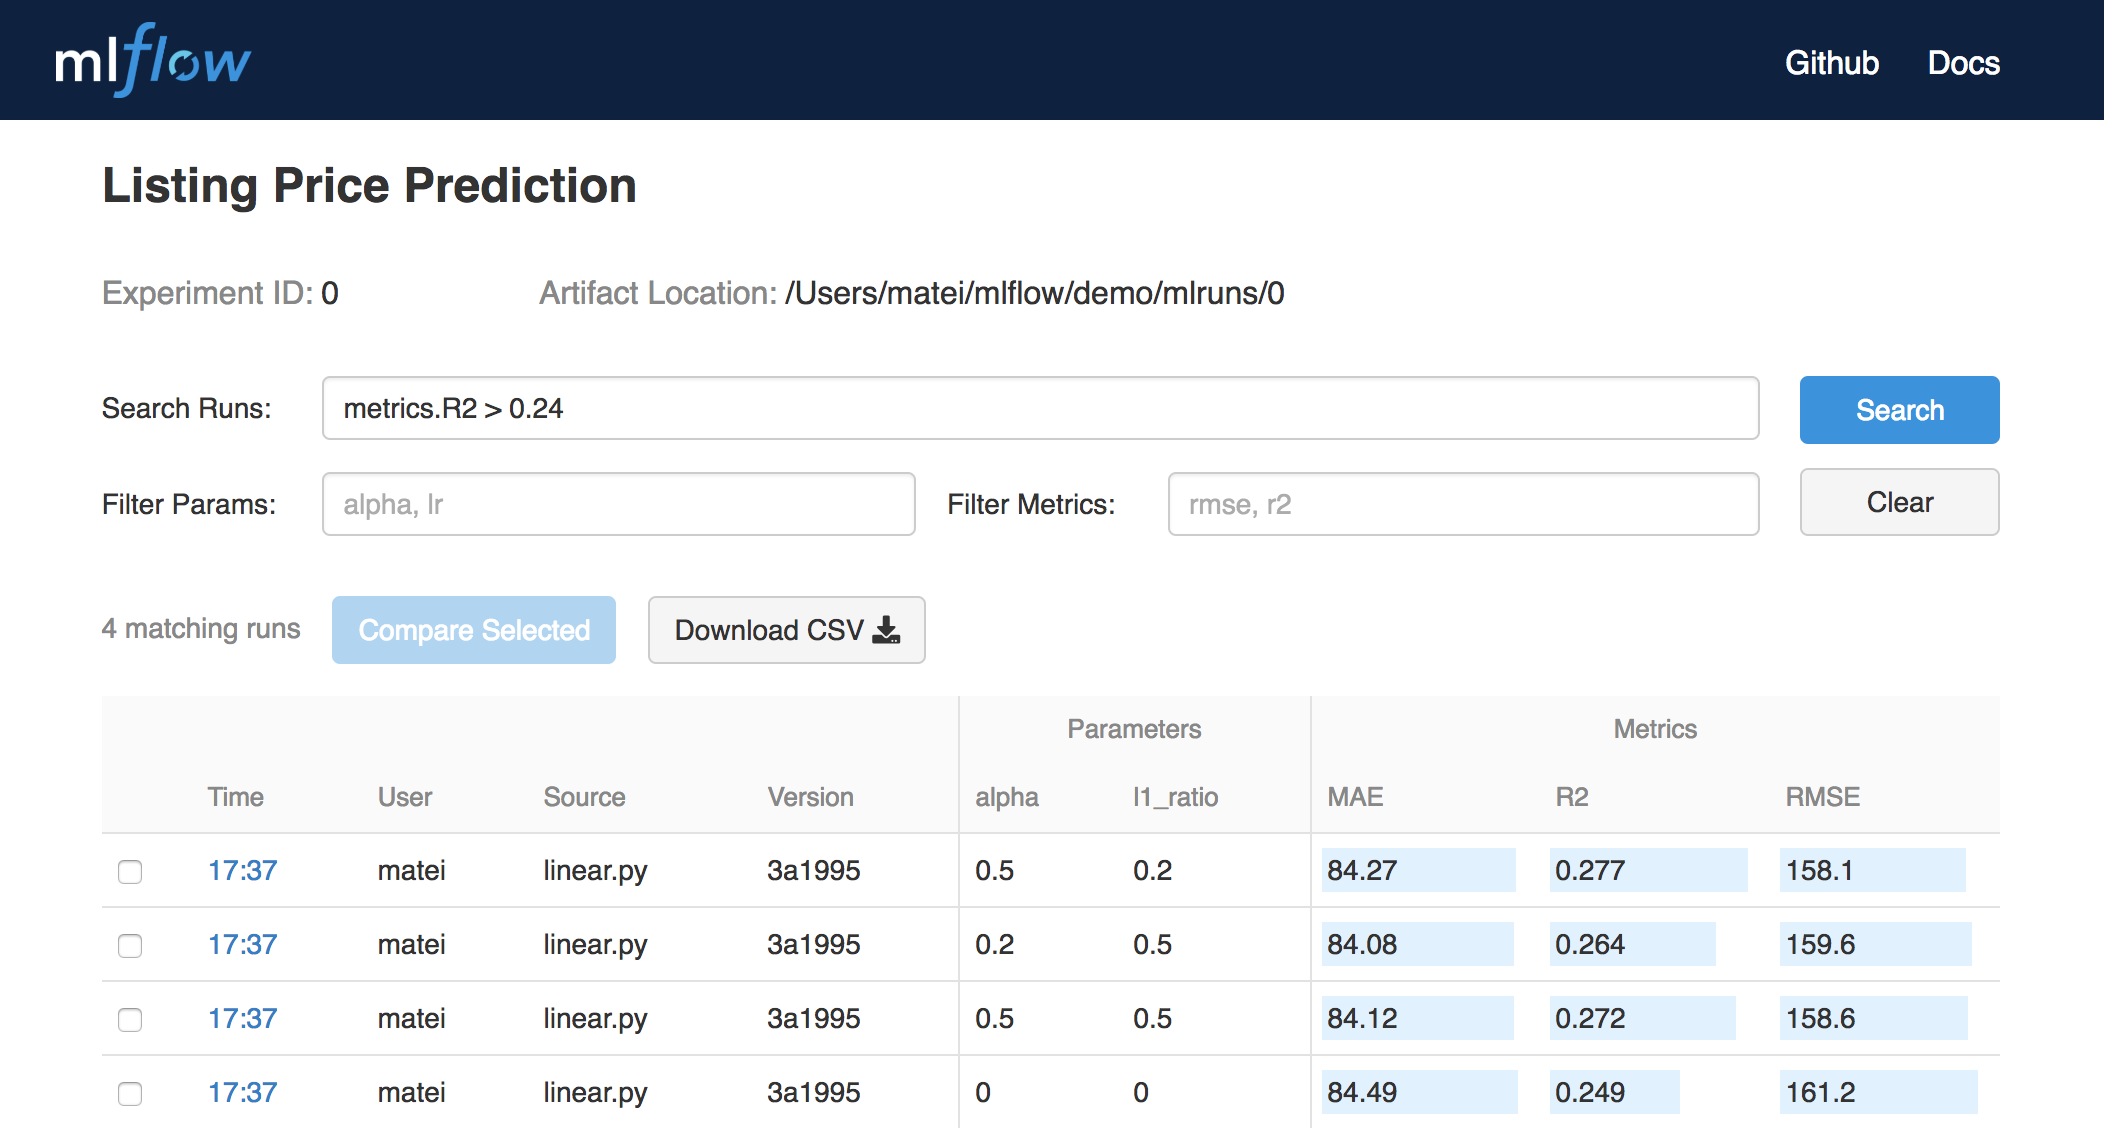
\includegraphics[bb=0 0 1052 564,width=\textwidth]{tracking.png}
\caption{MLflow Tracking UI showing several runs in an experiment. Clicking each run lists its metrics, artifacts and output details and lets the user post comments about the run.}
\label{fig:tracking-ui}
\end{figure}

\subsection{MLflow Projects}

MLflow Projects provide a simple format for packaging reproducible data science code. Each project is simply a directory with code or a Git repository, and uses a descriptor file to specify its dependencies and how to run the code. A MLflow Project is defined by a simple YAML file called MLproject, as shown below:

\begin{Verbatim}[frame=single,fontsize=\small,samepage=true]
name: My Project
conda_env: conda.yaml
entry_points:
  main:
    parameters:
      data_file: path
      alpha: {type: float, default: 0.1}
    command: "python train.py --reg-param {alpha} --data {data_file}"
\end{Verbatim}


Projects can specify their dependencies through a Conda environment or (in an upcoming release) a Docker container specification. A project may also have multiple entry points for invoking runs, with named parameters that downstream users can provide without understanding the internals of the project.

Users can run projects using the \texttt{mlflow run} command line tool, either from local files or a Git repository:

\begin{Verbatim}[frame=single,fontsize=\small,samepage=true]
mlflow run git@github.com:databricks/mlflow-example.git -P alpha=0.5
\end{Verbatim}

Alternatively, projects can be called programmatically using MLflow's API. This can be used to implement multi-step workflows or to pass projects a ``black box'' into automated tools such as hyperparameter search~\cite{hyperopt}.

In either case, MLflow will automatically set up the project's runtime environment and execute it. If the code inside the project uses the MLflow Tracking API, MLflow will also remember the project version executed (that is, the Git commit) and show an \texttt{mlflow run} command to re-execute it in its UI. Finally, MLflow projects can also be submitted to cloud platforms such as Databricks for remote execution.

\subsection{MLflow Models}

MLflow Models are a convention for packaging machine learning models in multiple formats called ``flavors'', allowing diverse tools to understand the model at different levels of abstractions. MLflow also offers a variety of built-in tools to deploy models in its standard favors. For example, the same model can be deployed as a Docker container for REST serving, as an Apache Spark user-defined function (UDF) for batch inference, or into cloud-managed serving platforms like Amazon SageMaker and Azure ML.

Each MLflow Model is simply stored as a directory containing arbitrary files and an MLmodel YAML file that lists the flavors it can be used in and additional metadata about how it was created:

\begin{Verbatim}[frame=single,fontsize=\small,samepage=true]
time_created: 2018-02-21T13:21:34.12
run_id: c4b65fc2c57f4b6d80c6e58a9dcb9f01
flavors:
  sklearn:
    sklearn_version: 0.19.1
    pickled_model: model.pkl
  python_function:
    loader_module: mlflow.sklearn
    pickled_model: model.pkl
\end{Verbatim}

In this example, the model can be used with tools that support either the \texttt{sklearn} or \texttt{python\_function} model flavors. For example, the MLflow SciKit-Learn library knows how to load a \texttt{sklearn} model as a SciKit-Learn Python object, but other deployment tools, such as running the model in a Docker HTTP server, only understand lower-level flavors like \texttt{python\_function}.
In addition, models logged using MLflow Tracking APIs will automatically include a reference to that run's unique ID, letting users discover how they were built.

\section{Example Use Cases}

In this section, we describe three sample MLflow use cases to highlight how users can leverage each component.

\vspace{-0.6em}
\paragraph{Experiment tracking.} A European energy company is using MLflow to track and update hundreds of energy grid models. This team's goal is to build a time series model for every major energy producer (e.g., power plant) and consumer (e.g., factory), monitor these using standard metrics, and combine the predictions to drive business processes such as pricing. Because a single team is responsible for hundreds of models, possibly using different ML libraries, it was important to have a standard development and tracking process. The team has standardized on using Jupyter notebooks for development, MLflow Tracking for metrics, and Databricks jobs for inference.

\vspace{-0.6em}
\paragraph{Reproducible projects.} An online marketplace is using MLflow Projects to package deep learning jobs using Keras and run them in the cloud. Each data scientist develops models locally on his or her laptop using a small dataset, checks them into a Git repository with an MLproject file, and submits remote runs of the project to GPU instances in the cloud for large-scale training or hyperparameter search. Using MLflow Projects makes it easy to create the same software environment in the cloud and share project code between different data scientists.

\vspace{-0.6em}
\paragraph{Model packaging.} The data science team at an e-commerce site is using MLflow Models to package recommendation models for use by application engineers. The technical challenge here was that the recommendation application includes both a standard, ``off-the-shelf'' recommendation model and custom business logic for pre- and post-processing. For example, the application might include custom code to make sure that the recommended items are diverse. This business logic needs to change in sync with the model, and the data science team wants to control both the business logic and the model, without having to submit a patch to the web application each time this logic has to change.
Moreover, the team wants to A/B test distinct models with distinct versions of the processing logic.
The solution was to package both the recommendation model and the custom logic using the \texttt{python\_function} flavor in an MLflow Model, which can then be deployed and tested as a single unit. %This allows production engineers to deploy the recommendation code as they please without the processing logic falling out of sync with the model.

\section{Related Work}

Many software systems aim to simplify ML development.
The closest to our work are the end-to-end ``ML platforms'' at large web companies.
For example, Facebook's FBLearner lets users write reusable workflow steps that run over data in Apache Hive~\cite{fblearner};
Uber's Michelangelo gives users a toolkit of algorithms to choose from that it can automatically train and deploy~\cite{michelangelo}; and Google's TFX provides data preparation and serving tools around TensorFlow~\cite{tfx}.
Anecdotally, these platforms greatly accelerate ML development, showing the benefits of standardizing the ML lifecycle.
However, they generally restrict users to a specific set of algorithms or libraries, so teams are on their own when they step outside these boundaries.
Our goal in MLflow is to let users easily bring their own tools and software in as many steps in the process as possible through our ``open interface'' design.
This includes custom training steps, inference code, and logged parameters and artifacts.

Other systems also tackle specific problems within the ML lifecycle. For example, Sacred~\cite{sacred}, ModelDB~\cite{modeldb} and TensorBoard~\cite{tensorboard} let users track experiments; PMML~\cite{pmml} and ONNX~\cite{onnx} are cross-library model serialization formats; Clipper~\cite{clipper} can deploy arbitrary models as Docker containers; and CDE~\cite{cde}, CodaLab~\cite{codalab}, Binder~\cite{binder} and Repo2Docker~\cite{repo2docker} enable reproducible software runs. MLflow combines these concepts with new ones, such as multi-flavor model packaging, into a unified system design and API.

\section{Conclusion}

For machine learning to have widespread commercial impact, organizations require the same kinds of reliable engineering processes around ML that exist in other engineering disciplines such as software development. In this paper, we have described some of the key challenges that differentiate ML development from traditional software development, such as experimentation, reproducibility, and reliable production deployment. We have also described MLflow, a software platform that can structure the machine learning lifecycle while giving users broad flexibility to use their own ML algorithms, software libraries and development processes.
MLflow is available as open source software at \url{https://www.mlflow.org}.


{\small

\begin{thebibliography}{10}

  \bibitem{abadi2016tensorflow}
  M.~Abadi, P.~Barham, J.~Chen, Z.~Chen, A.~Davis, J.~Dean, M.~Devin,
    S.~Ghemawat, G.~Irving, M.~Isard, et~al.
  \newblock {TensorFlow: A System for Large-Scale Machine Learning}.
  \newblock In {\em OSDI}, volume~16, pages 265--283, 2016.

  \bibitem{tfx}
  D.~Baylor, E.~Breck, H.-T. Cheng, N.~Fiedel, C.~Y. Foo, Z.~Haque, S.~Haykal,
    M.~Ispir, V.~Jain, L.~Koc, C.~Y. Koo, L.~Lew, C.~Mewald, A.~N. Modi,
    N.~Polyzotis, S.~Ramesh, S.~Roy, S.~E. Whang, M.~Wicke, J.~Wilkiewicz,
    X.~Zhang, and M.~Zinkevich.
  \newblock Tfx: A tensorflow-based production-scale machine learning platform.
  \newblock In {\em Proceedings of the 23rd ACM SIGKDD International Conference
    on Knowledge Discovery and Data Mining}, KDD '17, pages 1387--1395, New York,
    NY, USA, 2017. ACM.

  \bibitem{hyperopt}
  J.~Bergstra, B.~Komer, C.~Eliasmith, D.~Yamins, and D.~D. Cox.
  \newblock Hyperopt: a python library for model selection and hyperparameter
    optimization.
  \newblock {\em Computational Science and Discovery}, 8(1):014008, 2015.

  \bibitem{binder}
  {Binder}.
  \newblock \url{https://mybinder.org}, 2018.

  \bibitem{clipper}
  D.~Crankshaw, X.~Wang, G.~Zhou, M.~J. Franklin, J.~E. Gonzalez, and I.~Stoica.
  \newblock Clipper: A low-latency online prediction serving system.
  \newblock In {\em Proceedings of the 14th USENIX Conference on Networked
    Systems Design and Implementation}, NSDI'17, pages 613--627, Berkeley, CA,
    USA, 2017. USENIX Association.

  \bibitem{fblearner}
  J.~Dunn.
  \newblock Introducing {FBLearner Flow}: Facebook’s {AI} backbone.
  \newblock
    \url{https://code.fb.com/core-data/introducing-fblearner-flow-facebook-s-ai-backbone/}.

  \bibitem{repo2docker}
  J.~Forde, T.~Head, C.~Holdgraf, Y.~Panda, G.~Nalvarte, M.~Pacer, F.~Perez,
    B.~Ragan-Kelley, and E.~Sundell.
  \newblock Reproducible research environments with repo2docker.
  \newblock ICML, 07/2018 2018.

  \bibitem{tensorboard}
  Google.
  \newblock Tensorboard: Visualizing learning.
  \newblock \url{https://www.tensorflow.org/guide/summaries_and_tensorboard}.

  \bibitem{pmml}
  A.~Guazzelli, W.-C. Lin, and T.~Jena.
  \newblock {\em PMML in Action: Unleashing the Power of Open Standards for Data
    Mining and Predictive Analytics}.
  \newblock CreateSpace, Paramount, CA, 2nd edition, 2012.

  \bibitem{cde}
  P.~J. Guo.
  \newblock {CDE}: A tool for creating portable experimental software packages.
  \newblock {\em Computing in Science and Engineering}, 14(4):32--35, 2012.

  \bibitem{michelangelo}
  J.~Hermann and M.~D. Balso.
  \newblock Meet {Michelangelo}: Uber’s machine learning platform.
  \newblock \url{https://eng.uber.com/michelangelo/}.

  \bibitem{sacred}
  {K}laus {G}reff, {A}aron {K}lein, {M}artin {C}hovanec, {F}rank {H}utter, and
    {J}\"urgen {S}chmidhuber.
  \newblock {T}he {S}acred {I}nfrastructure for {C}omputational {R}esearch.
  \newblock In {K}aty {H}uff, {D}avid {L}ippa, {D}illon {N}iederhut, and
    M.~{P}acer, editors, {\em {P}roceedings of the 16th {P}ython in {S}cience
    {C}onference}, pages 49 -- 56, 2017.

  \bibitem{codalab}
  P.~Liang et~al.
  \newblock {CodaLab}.
  \newblock \url{https://worksheets.codalab.org}, 2018.

  \bibitem{onnx}
  {ONNX Group}.
  \newblock {ONNX}.
  \newblock \url{https://onnx.ai}.

  \bibitem{modeldb}
  M.~Vartak, H.~Subramanyam, W.-E. Lee, S.~Viswanathan, S.~Husnoo, S.~Madden, and
    M.~Zaharia.
  \newblock Modeldb: A system for machine learning model management.
  \newblock In {\em Proceedings of the Workshop on Human-In-the-Loop Data
    Analytics}, HILDA '16, pages 14:1--14:3, New York, NY, USA, 2016. ACM.

  \end{thebibliography}


}
%\bibliographystyle{abbrv}
%\bibliography{paper}

\end{document}

\end{article}

\begin{article}
{Networking and Storage: The Next Computing Elements inExascale Systems?}
{Alberto Lerner, Rana Hussein, Andre Ryser, Sangjin Lee, Philippe Cudre-Mauroux}
\graphicspath{{submissions/alberto/figs/}}
\documentclass[11pt,dvipdfmx]{article}

%\usepackage{deauthor}
%\usepackage{times}
%\usepackage{graphicx}

\newcommand{\softsubsec}[1]{\vspace{0.6em}\noindent\textbf{#1}}
\newcommand{\softsec}[1]{\vspace{1em}\noindent\textbf{#1}}

%\graphicspath{{./submissions/alberto/figs/}}

\begin{document}

\title{Networking and Storage: The Next Computing Elements in Exascale Systems?}

\author{Alberto Lerner$^1$~~~~Rana Hussein$^1$~~~~Andr\'{e} Ryser$^1$~~~~Sangjin Lee$^2$\thanks{Work done while visiting the University of Fribourg.}~~~~Philippe Cudr\'{e}-Mauroux$^1$  \vspace{0.4em} \\$^1$\emph{University of Fribourg~~~~~~~~~~~~$^2$Hanyang University} \\ \emph{Switzerland~~~~~~~~~~~~~~~~~~~~~~~~~~~~~South Korea}}

\maketitle

\begin{abstract}
Many large computer clusters offer alternative computing elements in addition to
general-purpose CPUs.
GPU and FPGAs are very common choices.
Two emerging technologies can further widen the options in that context: in-network
computing (INC) and near-storage processing (NSP).
These technologies support computing over data that is in transit between nodes
or inside the storage stack, respectively.
There are several advantages to moving computations to INC and NSP platforms.
Notably, the original computation path does not need to be altered to
route data through these subsystems; the network and the storage are naturally
present in most computations.


In this paper, we describe the evolutionary steps that led to INC and NSP platforms
and discuss how they can improve critical computing paths in large-scale
database systems.
In the process, we comment on the constraints that the current generation of
these platforms present as well as expose why we believe them to be relevant
to the next generation of exascale platforms.
\end{abstract}


\section{Motivation}
\label{sec:motivation}

\begin{figure}[t]
    \centering
    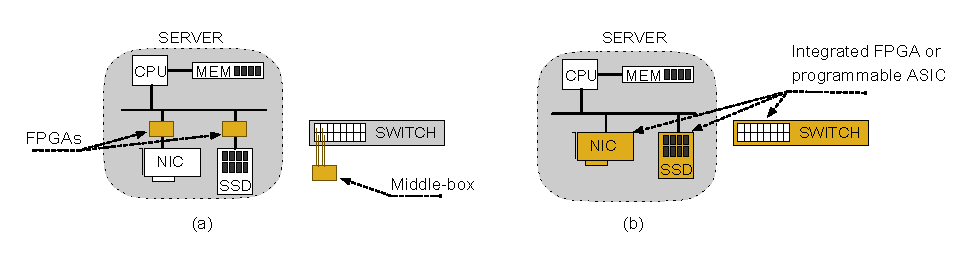
\includegraphics[bb=0 0 451 108]{fig_bump_internal.eps} %% 0.75
    \caption{Alternative in-network computing and near-storage processing
      platforms.
      (a) Using ``bump-in-the-wire'' FPGAs or network ``middle-boxes'' to create
      early application logic sites.
      (b) Leveraging programmability within the device for application logic.}
    \label{fig:bump_internal}
\end{figure}


The networking and storage stacks have always carried some computing power.
Network switches can triage billions of packets per second.
Solid-state drives (SSDs) can scramble and encode gigabytes of data per second
(for error correction purposes~\cite{cai17}).
Despite such computing power, applications have no access to how the
devices process the data, other than by issuing IO requests.
The functionality of these devices has been closed to changes.  Opening them
would require supporting a certain level of \emph{programmability}.


Nonetheless, the benefits of executing application logic close to networking and
storage devices are known~\cite{fang19, teubner13}.
New algorithms that take advantage of proximity to the data become viable and
provide both performance and power consumption gains.
Figure~\ref{fig:bump_internal}(a) illustrates how FPGAs and network
``middle-boxes'' can create these opportunities.


The lack of programmability in network and storage devices has impacted not
only applications.
It has also hindered the advancement of these platforms.
On the networking side, new protocols emerge that depend heavily on hardware to
run at high-speeds.
\emph{Fixed-function} devices, the ones that have their functionality ``baked''
into the hardware, may need to undergo a full, lengthy development cycle before
they can run new protocols.
Recently, a solution emerged where a new class of networking devices started
supporting programmability (e.g., in programmable switches~\cite{bosshart13} and
``smart'' NICs~\cite{zilberman14}).
The protocols these devices run are expressed as software programs.


The need for programmability also emerged on storage platforms recently.
SSDs are designed to shield applications from the intricacies of managing
flash memory.
However, evidence appeared that SSDs often miss the right performance decisions
because of the separation between it and the
applications~\cite{bjorling17}.
A more \emph{modular} SSD design, deemed \emph{open-channel}, was proposed that
allows a host (a server), rather than the SSD itself, to make certain low-level
decisions.
The modules that run on the host are software-based, therefore programmable.


Developers soon realized that the programmability could also be used by
applications.
It made it possible to inject application code directly into the networking and
storage stacks.
Figure~\ref{fig:bump_internal}(b) depicts such a scenario.
\emph{In-network computing} and \emph{near-storage processing} emerged as the
disciplines that leverage processing power in the network and storage stacks,
respectively, for application purposes.


An application that benefits from INC or NSP contains, by definition, algorithms
running in different computing elements of a system.
These algorithms ought to communicate at high speed.
The most commonly used interconnect for such systems has been based on the
PCIe bus standard~\cite{budruk03}.
At this time, the standard is being revised to operate at higher speeds.
PCIe is also being extended with mechanisms to support cache coherence protocols
to run atop of it~\cite{ccix19, cxl19}.


Despite their potential, INC and NSP platforms are not without challenges.
INC is a more mature technology with increasingly popular programmable models
that shield the developer from the intricacies of the devices.
Such programming models, however, are quite different from a general-purpose
CPU’s.
In contrast, NSP often uses general-purpose processors---but much less powerful
ones than server-class CPUs.
In both cases, porting algorithms to these platforms requires rethinking the
algorithms to fit either a different model or a less-powerful environment.


In this paper, we elaborate on the above challenges and opportunities of
adopting INC and NSP as platforms to improve application performance.
We summarize the contributions of this paper are as follows:
\begin{itemize}
  \setlength{\itemsep}{0pt}
  \setlength{\parsep}{0pt}
  \setlength{\parskip}{0pt}
  \setlength{\topsep}{0pt}
  \setlength{\partopsep}{0pt}
\item We discuss the evolution and recent advancements of INC and NSP platforms;
\item We present specific computation tasks that can benefit from them;
\item We describe the challenges that still remain in order to use INC and NSP
  as application platforms;
\item Finally, we present the benefits of adopting the current generation of INC
  and NSP.
\end{itemize}


The rest of this paper is structured as follows.
We discuss the programmability of the network and storage stacks in more detail
in Section~\ref{sec:background}.
We show examples of computing paths that can leverage INC and NSP capabilities in
Section~\ref{sec:data_paths}.
We comment on the evolution of the PCIe interconnect and the possibilities it
opens in Section~\ref{sec:interconnects}.
We discuss the challenges and opportunities of adopting INC and NSP platforms in
Section~\ref{sec:challenges}.
We elaborate on how ready for adoption the technologies are in
Section~\ref{sec:discussion}, before concluding in Section~\ref{sec:conclusion}.


\section{An Abridged History of INC and NSP}
\label{sec:background}

There have been many attempts to conciliate speed and flexibility in
networking hardware devices.
Figure~\ref{fig:evolution_net} depicts the main ideas behind the relevant
milestones in that context.


\begin{figure}[h]
  \centering
  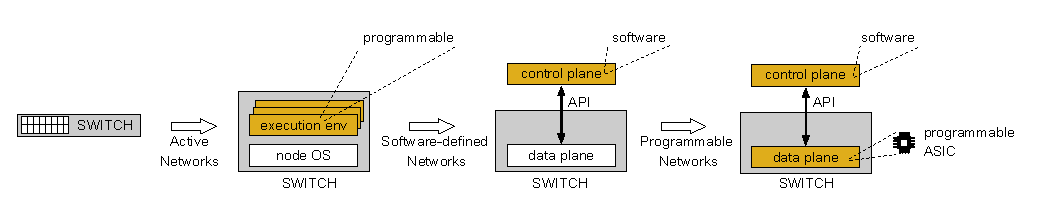
\includegraphics[bb=0 0 483 88]{fig_evolution_net.eps} %% 0.68
  \caption{Evolution of the network stack towards programmability.}
  \label{fig:evolution_net}
\end{figure}


\emph{Active Networks}, one of the first attempts, proposed a standard
architecture for more flexible network devices~\cite{calvert98}.
The goal of the architecture is to enable changes to the device
behavior—--typically to implement new protocols—--via the execution of
user-driven customization.
There are two main components in such a device.
First, a node operating system that manages basic IO functionality, including
processing, storage, and transmission.
Second, multiple Execution Environments (EE) that support the execution of
programs containing packet-processing logic.
Applications can inject code into the device through an API, which generates
special packets for the device to execute.
Active networks proved to be very flexible; however, they ran considerably
slower than their fixed-function counterparts.


\emph{Software-Defined Networks} (SDN), a later attempt at a more flexible
network, is also centered around a standard device
architecture~\cite{kreutz15}.
The main feature of the architecture is the separation of the control plane
(policy definition) from the data plane (policy implementation).
The control plane would contain information such as routing tables; the data
plane would use that information to forward packets without sacrificing speed.
An SDN device could adopt a new protocol if the SDN standard recognizes that
protocol.
Introducing new protocols, however, still required changes in the SDN standard
itself and sometimes also on the devices.
The main issue was that SDN only supports custom logic on the control plane.
Protocols that depended on special per-packet logic need to send these packets
to the control plane, which in turn processes them, pushing the results back to
the data plane.
The additional path cannot sustain \emph{line-rate}, as one calls the individual
port speed of a switch.


In a more recent development, \emph{Programmable Dataplanes} (also referred to
as \emph{Programmable Networks}) allowed custom logic on the data
plane~\cite{bifulco18}.
The cornerstone of this technology is a generation of programmable ASICs (chips)
that supports a certain degree of stateful packet processing without compromising
speed~\cite{bosshart13}.
This balance is captured by a programming model called Protocol Independent
Switch Architecture (PISA)~\cite{sivaraman16}.
PISA shields the programmer from various device intricacies and, because it was
designed to be protocol-independent, it proved adept at expressing application
computations as well.
Programmable networks created the conditions for a new generation of
applications to push specialized logic into the network, i.e., to perform
\emph{in-network computing}.


\vspace{1em}
We now turn our attention to the evolution of the storage stack.
Just as with networks, the idea of near-storage processing is not new, but the
driver for altering this stack has been more application-centric than in
networking.
In the early 2000s, a seminal proposal, called \emph{Active Disks}, gained
traction that aimed at transforming hard drive controllers into data-processing
platforms~\cite{riedel01}.
These controllers often carried a small, general-purpose processor that was
somewhat over-dimensioned for its purpose.
Applications could place logic on that processor, and access/modify the data
blocks that were streaming in and out of the hard drive.
The computing power of these controllers ultimately proved to be underwhelming,
and the industry saw little need to improve them.


Eventually, SSDs based on NAND-flash displaced hard drives in many applications.
Managing flash memory requires considerably more computing power than a magnetic
medium, and flash memory error rates are very high, which requires
computational-intensive error correction techniques~\cite{cai17}.
Moreover, the industry decided that SSDs should be drop-in replacements for hard
drives.
SSDs execute internally a compatibility layer called Flash Translation Layer
(FTL) for that purpose~\cite{chung09}.
All these factors turn SSDs into relatively powerful embedded devices.


A proposal soon emerged to leverage SSD controllers for database query
processing using \emph{smart SSDs}~\cite{do13}.
As with active disks, the computing capacity on early devices was not sufficient
for most computations in practice~\cite{do19}.
It would take a new generation of devices to accommodate fast database
logic~\cite{kim16}.
However, the industry focus was more on making devices faster than on making
them smarter.
Performance wasting was an issue, as the FTL not always makes the best decisions
from an application's point of view.
Some efforts emerged that tried to make SSD architectures more open to
configurations.
Figure~\ref{fig:evolution_ssd} captures the essential steps of this effort.


\begin{figure}[h]
  \centering
  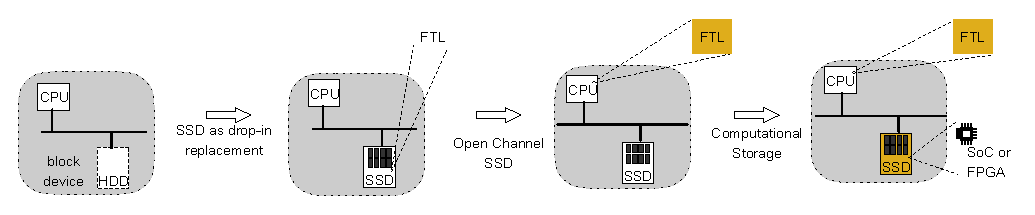
\includegraphics[bb=0 0 481 87]{fig_evolution_ssd.eps} %% 0.68
  \caption{Evolution of the storage stack towards programmability.}
  \label{fig:evolution_ssd}
\end{figure}

\emph{Open Channel SSDs} appeared from a growing understanding that many of the
FTL tasks were better performed leveraging application
knowledge~\cite{bjorling17}.
In an open-channel SSD, some of the FTL responsibilities are removed from the
device.
Instead, they run on the host housing the SSD or even inside individual
applications~\cite{ouyang14}.
Naturally, these devices expose a lower-layer view of the underlying flash
medium.


With more exposure to SSD architectural details, several works emerged to build
tooling around these devices.
These efforts range from frameworks to program SSD controllers~\cite{picoli20},
to performance measurement tooling~\cite{lerner20}, to even full SSD rapid
prototyping platforms~\cite{kwak20}.
At the same time, a class of works appeared that deploy application code on
SSDs, making them a \emph{Computational Storage} platform~\cite{picoli19, ruan19,
woods14}.
The common thread in these works is that they increase the existing computing
power of the devices by building them on platforms such as a System-on-a-Chip
(SoC) or an FPGA.
The tooling and the additional computing capacity paved the way for
\emph{Near-Storage Processing}.


One problem that remains open, however, is the lack of a consensus around a
programming model.
While there are recent proposals in that sense (e.g., in~\cite{gu16}), these
models leave many aspects undefined.
For instance, they have not addressed how to interface application logic with
internal device mechanisms.
An application that wishes to influence the IO scheduling policy of a device
directly has no means to do so.
There is also no consensus on how to shield an application developer from
specific aspects of different devices.


\section{Alternative Computing Paths}
\label{sec:data_paths}

INC and NSP  provide alternative sites beyond a CPU where applications can place
logic.
This fundamentally changes the traditional data movement patterns we see in
CPU-centric algorithms, potentially bringing performance and power savings
benefits.
We illustrate these possibilities in this section by presenting and discussing
several use cases in large-scale data management.


\subsection{In-Network Data Aggregation}
\label{ssec:aggr}

Data aggregation is a very common operation in data management.
Aggregation involves grouping data by specific criteria and calculating
summaries over each group.
A typical example is the \texttt{GROUP BY} clause in \texttt{SQL}.
When the data volume is large, the operation can involve several servers,
e.g., as in a rack-wide computation.
Figure~\ref{fig:flow_1}(a) illustrates one possible way to solve such a distributed
aggregation.


The servers agree on how to partition the data, taking into consideration the
grouping key.
This divides the work into disjoint, independent tasks.
Each server reshuffles its data while performing the aggregation over its
assigned partition, as data arrives.
Eventually, all the machines send their aggregation results to an elected
server, which combines them into a global result.
Note that throughout all these interactions, the switch performs data
transmissions only.


\begin{figure}[h]
    \centering
    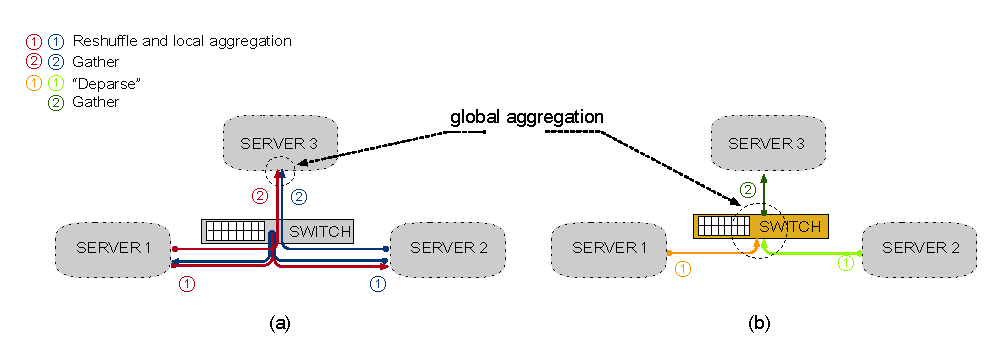
\includegraphics[bb=0 0 462 156]{fig_flow_1.eps} %% 0.75
    \caption{Data aggregation scenario (e.g., SQL GROUP BY).
      (a) With a ``passive'' switch, the servers first repartition the data
      and work on aggregating its assigned partition locally.
      Then, an elected server gathers all partitions and performs the global
      aggregation.
      (b) On an INC platform, an ``active'' switch can, in typical situations,
      perform the global aggregation in one step and transmit the results to an
      elected server.
      We use a given color to represent each unique data stream in the
      computation.
      }
    \label{fig:flow_1}
\end{figure}


In Figure~\ref{fig:flow_1}(b), we show that using the switch as an active
element simplifies the entire computing path~\cite{lerner19}.
We assume that the switch is programmable and that it can be leveraged to hold
an entire aggregation table.
The size of such a table is often manageable, as it is proportional to the
number of groups involved, rather than the size of the dataset.
Note that the servers need not reshuffle the data nor perform an aggregation on
a partition.
Because programmable switches perform computations at line-speed, the
aggregation table on the switch will be completed as soon as the last server
finishes transmitting its tuples, and can then be sent immediately to an elected
server.


Not all computations are suitable for INC deployment.
The important caveats include: (a) the number of steps the switch can execute
over each packet is limited; (b) the kind of instructions the switch can perform
is also constrained; and (c) programmable network devices adhere to a
programming model that imposes a \emph{forward logic}-style onto algorithm
design.
Loops and complex branching are strongly discouraged, although possible.
In practice, these restrictions reduce the choices of data structures the switch
can support.
In particular, the aggregation described in Figure~\ref{fig:flow_1}(b) requires
a hash table to be adapted to INC constraints.
In this case, the number of collisions can be handled on the switch up to a
certain bound.
Relaxing this constraint involves using a technique called
``overflowing''~\cite{lerner19}, which allows treating long collision chains
outside the switch without a noticeable performance penalty in most cases.

These limitations notwithstanding, a large class of computations can benefit from
INC platforms~\cite{ports19}.
Moreover, processing data on the switch tends to scale well as the number of
servers grows in the cluster.
The number of switches naturally grows with the number of servers.


\subsection{Near-Storage Checkpoint Derivation}
\label{ssec:cp_derivation}

We now describe an opportunity that arises specifically in an in-memory database
system.
Like most DBMSs, in-memory databases guarantee durability using a persistent
transaction log.
Because the log can get arbitrarily long, it would be impractical to recover
from a crash just by replaying it.
Therefore, databases also perform a periodical checkpoint (e.g., by taking a
snapshot) of the current memory state and write it to persistent storage, often
SSDs.
A recovery algorithm can load the snapshot and replay the portion of the log
acquired after the checkpoint.
In in-memory databases, the log and checkpoint are the only workloads written to
disk.


The logging and checkpointing processes compete for both disk and memory
bandwidth.
Figure~\ref{fig:flow_2}(a) shows these contention points.
The checkpointing process reads the database contents from the main-memory while
it is being queried/modified.
The checkpointing process also issues write requests to the SSD, which have to
be scheduled along with the logging workload.
The contention is responsible for the throughput reduction that many systems
experience during checkpoints.


\begin{figure}[h]
  \centering
  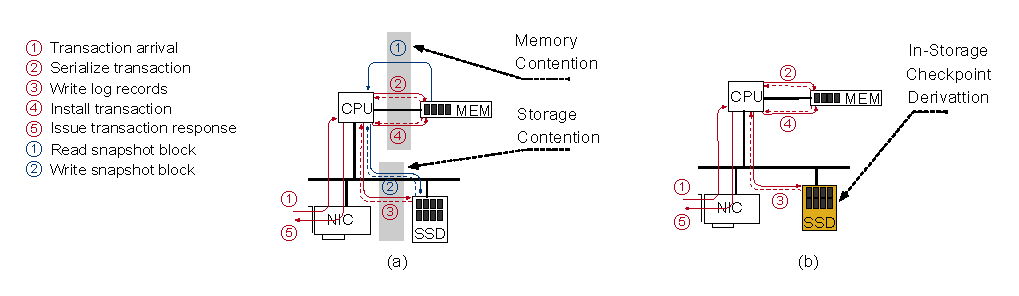
\includegraphics[bb=0 0 473 126]{fig_flow_2.eps} %% 0.75
  \caption{Checkpoint computation scenario.
    (a) Transaction logging (red) and checkpoint (blue) are two parallel
    processes.
    They compete for memory and disk bandwidth.
    (b) A checkpoint could be derived by processing the transaction log inside
    an SSD.
    The solid lines represent data; the dashed ones, control and/or return.
  }
  \label{fig:flow_2}
\end{figure}


The key observation here is that partial snapshots, which can serve as
checkpoints, can be derived from the log stream directly.
We believe that such derivations may very well occur inside a smart SSD.
We show in Figure~\ref{fig:flow_2}(b) that once we move that process to the
device, the contention points disappear.


Note, however, that the processing power on an SSD is far smaller than that of a
general-purpose CPU.
We cannot possibly expect to move the same algorithm we used on a CPU into an
NSP platform and obtain similar performance results.
Creating a checkpoint derivation algorithm for an SSD requires finding snapshot
approximations that the device can process at the necessary pace.
We comment on Section~\ref{sec:challenges} how specific architectural changes on
smart SSDs can make this task easier.


\subsection{Low Latency Database Replication}
\label{ssec:low_latency}


Another code path that can benefit from either INC or NSP is that of a replica
node in a database system.
On a master node, transactions need to be serialized via a concurrency control
algorithm.
The latter typically runs on a CPU.
The replica node code-path is simpler because the serial order of the
transactions was already determined.
The CPU takes the modifications coming from the network card and persists them
on disk in the same order it received them.
Subsequently, it updates its data structures and sends a notification to the
master node that it accepted the transaction.
Figure~\ref{fig:flow_3}(a) depicts such an interaction.


\begin{figure}[h]
  \centering
  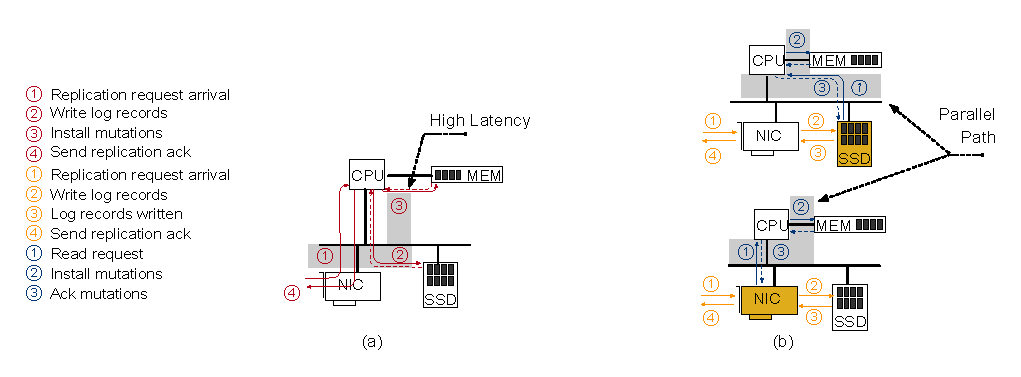
\includegraphics[bb=0 0 474 165]{fig_flow_3.eps} %% 0.75
  \caption{Database replica node scenario.
    (a) Each transaction log entry is first persisted in storage and then
    applied to memory, as the CPU coordinates the replication.
    (b) If an ``active'' NIC or SSD coordinates the process, the persistence and
    memory update paths can proceed in parallel.
  }
  \label{fig:flow_3}
\end{figure}


Note that the replica code path incurs in latency.
The master node may be withholding the original transaction until the
replication path is completed.
We can optimize this code path in at least two ways.
Using NSP, the NIC would send the modification stream directly to a smart SSD.
In turn, the SSD could be programmed to coordinate the interaction instead of
the CPU.
The SSD would notify the NIC after it persisted the changes, reducing the
latency.
It would also, in parallel, allow the CPU to read (and perform) the
modifications.
An alternative path exists where the NIC itself would perform the coordination.
Figure~\ref{fig:flow_3}(b) shows both cases.
This scenario involves having the NIC and the SSD communicate without any CPU
intervention.
This type of communication is called peer-to-peer DMA~\cite{budruk03} and it has
been used in other contexts before, such as direct access to a remote disk
(e.g., NVMe-over-Fabrics~\cite{guz18}).


\section{Upcoming Interconnects}
\label{sec:interconnects}

INC and NSP platforms rely on an interconnect to communicate with other
computing elements in a system.
PCIe has been the \emph{de facto} interconnect for quite a
while~\cite{budruk03}.
PCIe is a point-to-point bus with a variable number of lanes dedicated to
devices.
Each lane can transfer close to 1GB/s on the current standard version, Gen 3.
Cards attached to the bus can use 1$\times$, 2$\times$, 4$\times$, 8$\times$, or
16$\times$ lanes to achieve a theoretical maximum of 16 GB/s bidirectional
bandwidth.


Newer devices are creating the need for faster speeds.
For instance, the standard NIC port speeds are about to go from 100 Gb/s to 400
Gb/s, which a single Gen 3 PCIe slot can no longer support.
The PCIe standard had moved to 2 GB/s lanes on Gen 4.
The following iteration of the standard, Gen 5, brings 4 GB/s lanes with a
theoretical bi-directional bandwidth of 64GB/s for 16$\times$ device.


There is another compelling feature that new versions of PCIe buses will bring:
cache coherence.
This feature allows computing elements to negotiate who may be caching a given
portion of memory at any given time.
It also determines who has the license to write to that memory address.
Coordinating access to single memory address allows all the computing elements
to share a single view of memory, as Figure~\ref{fig:coherence}(a) shows.
There are two flavors of coherency: one in which the CPU has a prominent role in
controlling the memory, called \emph{asymmetric}, and one in which all computing
elements play a similar role, called \emph{symmetric}.


\begin{figure}[h]
  \centering
  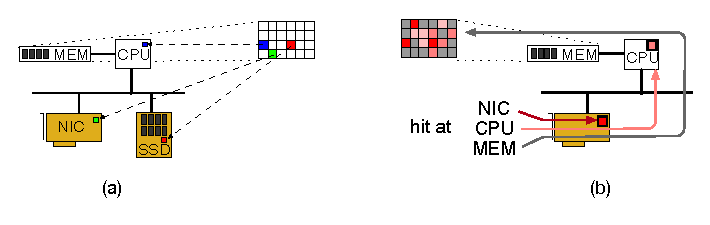
\includegraphics[bb=0 0 325 92]{fig_coherence.eps} %% 0.75
  \caption{Cache coherency scenarios: (a) a NIC and an SSD may be responsible
    for writing to specific addresses in memory that can be read by other
    elements, and (b) a NIC can be responsible for caching (and writing to) very
    hot pages while leaving the CPU responsible for less accessed pages.
  }
  \label{fig:coherence}
\end{figure}


At the time of writing, there are four upcoming interconnects offering both high speed and coherence:
CAPI~\cite{stuecheli15}, CCIX~\cite{ccix19}, CXL~\cite{cxl19} and
Gen-Z~\cite{knebel19}.
CCIX and Gen-Z support symmetric coherence, unlike CAPI or CXL, which support
asymmetric coherence.
CAPI is a competing standard to PCIe.
CCIX and CXL use only PCIe, while Gen-Z can use ethernet as well as PCIe.
The range of PCIe is short enough to work only within the confines of a chassis,
while ethernet allow to connect across chassis.
This opens up the possibility of CCIX or CXL being applied simultaneously with
Gen-Z to form coherence domains that cross server boundaries.


Cache coherency allows for new INC and NSP design use cases.
For instance, one may extend the caching hierarchy beyond the CPU.
Figure~\ref{fig:coherence}(b) illustrates this possibility.
Some distributed applications may cache hot data items in the
NIC~\cite{tokusashi18}.
With coherence, the NIC can also request write access to such an item and update
it.
Any other computing element that requests to cache that address would then see
the updates.


\section{Challenges and Opportunities}
\label{sec:challenges}

We mentioned above some immediate difficulties that arise when deploying current
generation INC and NSP platforms.
In this section, we elaborate on further challenges and opportunities that we
believe would unlock more of the potential of these platforms.


\softsubsec{In-Network Stateful Computations.}
%
Data management primarily involves stateful computations, i.e., algorithms that
access a result from a previous iteration and generate a new result at the
next one.
The aggregation operation discussed in Section~\ref{ssec:aggr} is one such
algorithm.
Maintaining state in-network, particularly in switches, is currently very
challenging.
Programmable switches rely on high-speed memories that, for cost reasons, are
present in limited amounts.
Moreover, switches have a very strict ``allowance'' of how many instructions
they can execute per packet and what those instructions can do.
These restrictions make maintaining data structures other than a hash
table on a switch possible but difficult.
Even some common operations on hash tables, such as collision management,
require some adapting, as we discussed above.


We miss a computing model that can relax those restrictions to a certain extent
while still keeping the ability to run logic at line-speed.
Supporting such a model would most likely require introducing new hardware onto
programmable switches.
We believe such a model is possible, but the field of in-network computing is
still new.
There is not yet a clear list of missing operations from applications beyond
networking protocols on which to base new switch hardware capabilities.


\softsubsec{SSD-Application Interface.}
%
A regular SSD makes several decisions such as IO scheduling and page mapping
based solely on observing the stream of IO commands it receives~\cite{nam11}.
When application logic executes inside the device, it becomes an additional
stream of IO commands.
The internal and external streams would likely compete with one another.
A straightforward way to manage the new internal streams is to pretend they came
from outside and to proceed as usual.


An alternative way would be to allow the application logic and the device to
interact.
Consider again the checkpoint derivation scenario we describe in
Section~\ref{ssec:cp_derivation}.
It generates new IO requests at a given pace.
Depending on the current load on the SSD, the checkpoint stream can be too fast or
too slow for the device to handle.
Ideally, we want a means for the device and the application logic to negotiate
that pace.
There is an opportunity here to establish a communication model that supports
this kind of interaction.


\softsubsec{SSD Channel Architecture.}
%
An SSD's bandwidth and capacity are a result of combining many relatively
limited NAND flash \emph{packages} (chips)~\cite{micheloni12}.
A typical arrangement is to group the packages in disjoint sets called
\emph{channels}.
There are anywhere between 8 to 32 channels in a typical SSD.
This arrangement has proved adequate when data pages are transferred in and out
of the device.


The introduction of application logic into an SSD, however, can cause data
pages to be moved \emph{across packages}---possibly between channels.
For instance, we describe in Section~\ref{ssec:cp_derivation} how an NSP process
can read pages from a transaction log and write them, after some manipulation,
as pages of a checkpoint.
In a traditional SSD architecture, this pattern would consume bandwidth from
both the origin and the destination channels.
We believe that there may be other package interconnect architectures
beyond channels that are more suited to the data movements above.
To the best of our knowledge, there has been no study about interconnects that
involve architectures other than fixed channels.


\softsubsec{Code-Variant Generation and Selection.}
%
INC and NSP platforms introduce additional hardware heterogeneity to computing
platforms.
An algorithm implementation that works well on a given switch may not work on a
different one, due to architectural differences.
The generation and selection of variant implementations is a known problem; it
appeared before in domains such as GPUs~\cite{rosenfeld15}.


To complicate matters, some algorithms are flexible enough to be deployed either
on a NIC or on the switch to which it connects.
The selection of the most appropriate platform constitutes an optimization step
that compounds to the variant selection problem above.
Currently, the programmer is responsible for making such choices.
There is an opportunity for creating higher-level tooling that would aid in
these decisions.


\softsubsec{Runtime Resource Management.}
%
In a regular setting, the operating system mediates every single network and
storage IO between applications and devices.
The OS does so by interposing itself between the two.
What, then, should be the role of the OS when a portion of the applications
reside \emph{inside} the device?


One potential solution is to accept that applications may want to access a device
directly, without mediation.
Such is the premise of Arrakis~\cite{peter15}, which tricks an application into
interacting with virtual versions of the devices, and redesigns the kernel to
provide the expected protections under such assumptions.


\section{Discussion}
\label{sec:discussion}

Notwithstanding the challenges and opportunities described in the previous
section, INC and NSP platforms are a reality.
The question arises as to whether they are ready for adoption.
In this section, we break this question into a list of sub-questions and answer
each one in turn.


\softsubsec{Are there diverse offerings of INC and NSP platforms?}
%
INC can be realized by many different hardware targets, both on switches and
NICs.
In terms of programmable switches, there are at least three silicon
manufacturers producing programmable ASICs: Barefoot (Intel)
Tofino~\cite{barefoot}, Broadcom Trident 4~\cite{broadcomT4}, and Cavium
(Marvel) Xpliant~\cite{cavium}.
Together, these chips appear in several commercial offerings from companies such as
Cisco and Arista.
SmartNICs are also widely available, ranging from FPGA-centric accelerators such as
Xilinx Alveo~\cite{xilinx} to more software-oriented platforms such as
Netronome~\cite{netronome}.
The offering for programming languages and abstractions is also diverse.
A prevalent language is \texttt{P4}~\cite{bosshart14}, but there are variations
such as \texttt{NPL}~\cite{broadcomnpl} and even \texttt{C} libraries in some
cases~\cite{netronome}.


NSP is also a rich environment with many prototyping and commercial platforms
available.
For instance, SSDs are starting to emerge that introduce application
specializations.
Samsung has recently announced the KV-SSD, which incorporates Key Value store
logic within its firmware~\cite{ki17}.
One issue with such offerings is that they add application functionality
but do not expose programmability.
The interested reader should look at~\cite{picoli20} for an extensive list of
specialized SSD and NSP-platforms available at the time of writing.


\softsubsec{What are the advantages of INC and NSP compared to ``CPU-centric''
alternatives?}
%
While there is no study yet of an exacale platform that resorts to both INC and
NSP, the expected benefits are a combination of increased performance, lower
energy expenditure, and lower CPU utilization.
There a numerous works that provide partial results.

For INC, data manipulations such as the one described in Section~\ref{ssec:aggr}
were studied before~\cite{lerner19}.
We can expect to see the performance of many typical queries improve by a factor of
2$\times$\ by using programmable switches at moderate network
speeds.
The power consumption in these switches is estimated to be only 12.4\% higher
than their fixed-function counterparts, and, anecdotally, the switches cost
about the same.
The operations-per-Watt ratio on some INC platforms such as smartNICs was
also studied before~\cite{tokusashi18}.
For instance, a variant of the caching scenario we discussed in
Section~\ref{sec:interconnects} reports a 17$\times$ better power utilization as
compared to a regular CPU.


NSP platforms deliver similar benefits.
According to~\cite{kim16}, the performance of scans and joins can see
performance improvements between 5$\times$ and 47$\times$, the cost of equipping
an SSD to support near-storage processing is less than 1\% of its total cost,
and the energy-efficiency compared to performing those operations on a CPU can be up
to 45$\times$ better.


\softsubsec{Are there standards in place to guarantee the portability and
longevity of the solutions?}
%
There is a big difference from a standardization point of view between INC and
NSP technologies.
As mentioned above, INC has broadly embraced \texttt{P4} as a programming language.
The latest edition of the language, \texttt{P4$_{16}$}, allows different target
platforms to express their capabilities.
A compiler can generate specific code from a unique source to different, maybe
even disparate, devices.
These feature makes the language flexible enough to work on future devices,
which can only help its adoption.


In contrast, there is not yet a consensus on how computational storage should be
programmed.
We even miss a standard around what an open-channel SSD should be, which would
arguably be a necessary step.


\section{Conclusion}
\label{sec:conclusion}

In this paper, we reviewed how the evolution of the network and storage stacks
have unlocked their computing power.
Applications can not only request services from these stacks, but also
embed logic into them.
We showed that with a careful redesign, algorithms running on INC or NSP
platforms could present a reduced amount of data movement, lower CPU
utilization, less energy consumption, or a combination of these.


We also discussed several challenges that INC and NSP still face.
Despite these limitations, we commented on a current generation of INC- and
NSP-enabled devices that are available off-the-shelf.
We believe that the emergence of the network and storage stacks as computing
elements creates promising ways to scale typical data management computations.


\softsec{Acknowledgments.}
%
This project has received funding from the European Research Council (ERC) under
the European Unions Horizon 2020 research and innovation programme (grant
agreement 683253/GraphInt).


\begin{thebibliography}{10}
\itemsep=1pt
\begin{small}

\bibitem{barefoot}
  \newblock Barefoot Tofino and Tofino 2 Switches.
  \newblock https://www.barefootnetworks.com/products/brief-tofino-2/.

\bibitem{bifulco18} R.~Bifulco, and G.~R\'etv\'ari.
  \newblock A Survey on the Programmable Data Plane: Abstractions, Architectures, and Open Problems.
  \newblock {\em HPSR}, June, 2018.

\bibitem{bjorling17} M.~Bj{\o}ling, J.~Gonz\'alez, and P.~Bonnet.
  \newblock Lightnvm: The Linux Open-Channel SSD Subsystem
  \newblock {\em FAST}, February, 2017.

\bibitem{broadcomnpl} Broadcom NPL.
  \newblock Network Programming Language.
  \newblock {\em https://nplang.org/}.

\bibitem{broadcomT4} Broadcom.
  \newblock Broadcom Trident 4.
  \newblock {\em https://www.broadcom.com/products/ethernet-connectivity/switching/strataxgs/bcm56880-series}.

\bibitem{bosshart13} P.~Bosshart, G.~Gibb, H.-S.~Kim, G.~Varghese, N.~McKeown, M.~Izzard, F.~Mujica, and M.~Horowitz.
  \newblock Forwarding Metamorphosis: Fast Programmable Match-Action Processing in Hardware for SDN.
  \newblock {\em SIGCOMM CCR}, 43(4):99--110, 2013.

\bibitem{bosshart14} P.~Bosshart., D.~Daly, G.~Gibb, M.~Izzard, N.~McKeown, J.~Rexford, C.~Schlesinger, D.~Talayco, A.~Vahdat, G.~Varghese, and D.~Walker.
  \newblock P4: Programming protocol-independent packet processors.
  \newblock {\em ACM SIGCOMM CCR}, 44(3):87--95, 2014.

\bibitem{budruk03} R.~Budruk, D.~Anderson, and E.~Solari.
  \newblock PCI Express System Architecture.
  \newblock {\em Pearson Education}, 2003.

\bibitem{cai17} Y.~Cai, S.~Ghhose, E.F.~Haratsch, Y.~Luo, and O.~Mutlu.
  \newblock Error Characterization, Mitigation, and Recovery in Flash-Memory-Based Solid-State Drives.
  \newblock {\em Proc. of the IEEE}, 105(9), 1666--1704, 2017.

\bibitem{calvert98} K.L.~Calvert, S.~Bhattacharjee, E.~Zegura, and J.~Sterbenz.
  \newblock Directions in Active Networks.
  \newblock {\em IEEE Comm. Magazine}, 36(10):72--78, 1998.

\bibitem{cavium} Cavium.
  \newblock XPliant Ethernet Switch Product Family.
  \newblock {\em www.cavium.com/XPliant-Ethernet-Switch-Product-Family.html}

\bibitem{ccix19} CCIX Consortium.
  \newblock An Introduction to CCIX.
  \newblock {\em White Paper}, https://www.ccixconsortium.com/wp-content/uploads/2019/11/CCIX-White-Paper-Rev111219.pdf

\bibitem{chung09} T.-S.~Chung, D.-J.~Park, S.~Park, D.-H.~Lee, S.-W.~Lee, and H.-J.~Song.
  \newblock A Survey of Flash Translation Layer.
  \newblock {\em J. of Syst. Archit.}, 55(5--6):332--343, 2009.

\bibitem{cxl19} D.D.~Sharma.
  \newblock An Introduction to Compute Express Link.
  \newblock {\em White Paper}, https://docs.wixstatic.com/ugd/0c1418\_d9878707bbb7427786b70c3c91d5fbd1.pdf.

\bibitem{do13} J.~Do, Y.S.~Kee, J.M.~Pzatel, C.~Park, K.~Park, and D.J.~DeWitt.
  \newblock Query Processing on Smart SSDs: Opportunities and Challenges.
  \newblock {\em SIGMOD}, June, 2013.

\bibitem{do19} J.~Do, S.~Sengupta, and S.~Swanson.
  \newblock Programmable Solid-State Storage in Future Could Datacenters.
  \newblock {\em CACM}, 62(6):54--62, 2019.

\bibitem{fang19} J.~Fang, Y.T.B.~Mulder, J.~Hidders, J.~Lee, and H.P.~Hofstee.
  \newblock In-Memory Database Acceleration on FPGAs: A Survey.
  \newblock {\em VLDB Journal}, October, 2019.

\bibitem{gu16} B.~Gu, A.S.~Yoon, D.H.~Bae, I.~Jo, J.~Lee, and J.~Yoon.
  \newblock Biscuit: A Framework for Near-Data Processing of Big Data Workloads.
  \newblock {\em SIGARCH Comp. Arch. News}, 44(3):153--165.

\bibitem{guz18} Z.~Guz, H.~Li, A.~Shayesteh, and V.~Balakrishnan.
  \newblock Performance Characterization of NVMe-over-Fabrics Storage Disaggregation.
  \newblock {\em ACM Trans. on Storage}, 14(4):1553--3077, 2018.

\bibitem{ki17} Y.-S.~Ki.
  \newblock Key Value SSD Explained – Concept, Device, System, and Standard.
  \newblock {\em SNIA SDC}, September, 2017.

\bibitem{kim16} S.~Kim, H.~Oh, C.~Park, S.~Cho, S.-W.~Lee, and B.~Moon.
  \newblock In-Storage Processing of Database Scans and Joins.
  \newblock {\em Inf. Sci.}, 327(C):183--200, 2016.

\bibitem{knebel19} P.~Knebel, D.~Berkram, A.~Davis, D.~Emmot, P.~Faraboschi, and G.~Gostin.
  \newblock Gen-Z Chipset for Exascale Fabrics.
  \newblock {\em HotChips}, August, 2019.

\bibitem{kreutz15} D.~Kreutz, F.M.V.~Ramos, P.E.~Ver\'issimo, C.E.~Rothenberg, S.~Azodolmolky, and S.~Uhlig.
  \newblock Software-Defined Networking: A Comprehensive Survey.
  \newblock {\em Proc. of the IEEE}, 103(1):14--76, 2015.

\bibitem{kwak20} J.~Kwak, S.~Lee, K.~Park, J.~Jeong, and Y.H.~Song.
  \newblock Cosmos+ OpenSSD: Rapid Prototype for Flash Storage Systems.
  \newblock {\em ACM Trans. on Storage}, to appear.

\bibitem{lerner19} A.~Lerner, R.~Russein, and P.~Cudr\'e-Mauroux.
  \newblock The Case for Network Accelerated Query Processing.
  \newblock {\em CIDR}, January, 2019.

\bibitem{lerner20} A.~Lerner, J.~Kwak, S.~Lee, K.~Park, Y.H.~Song, and P.~Cudr\'e-Mauroux.
  \newblock It Takes Two: Instrumenting the Interaction between In-Memory Databases and Solid-State Drives.
  \newblock {\em CIDR}, January, 2020.

\bibitem{micheloni12} R.~Micheloni, A.~Marelli, and S.~Eshghi.
  \newblock Inside Solid State Drives (SSDs).
  \newblock {\em Springer}, 2012.

\bibitem{nam11} E.H.~Nam, B. S. J.~Kim, H.~Eom, and S. L.~Min.
  \newblock Ozone (O3): An Out-of-Order Flash Memory Controller Architecture.
  \newblock {\em IEEE Transactions on Computers}, 60(5):653--666, 2011.

\bibitem{netronome} Netronome.
  \newblock Agilio CX SmartNICs.
  \newblock {\em https://www.netronome.com/products/agilio-cx/}

\bibitem{ouyang14} J.~Ouyang, S.~Lin, S.~Jiang, Z.~Hou, Y.~Wang, and Y.~Wang.
  \newblock SDF: Software-Defined Flash for Web-Scale Internet Storage Systems.
  \newblock {\em ASPLOS}, 2014.

\bibitem{peter15} S.~Peter, J.~Li, I.~Zhang, D.R.K.~Ports, D.~Woos, A.~Krishnamurthy, T.~Anderson, and T.~Roscoe.
  \newblock Arrakis: The Operating System Is the Control Plane.
  \newblock {\em ACM TOCS}, 33(4), 2015.

\bibitem{picoli19} I.L.~Picoli, P.~Bonnet, and P.~T\"oz\"un.
  \newblock LSM Management on Computational Storage.
  \newblock {\em DaMoN}, July, 2019.

\bibitem{picoli20} I.L.~Picoli, N.~Hedam, P.~Bonnet, and P.~T\"oz\"un.
  \newblock Open-Channel SSD (What Is It Good For).
  \newblock {\em CIDR}, January, 2020

\bibitem{ports19} D.R.K.~Ports, and J.~Nelson.
  \newblock When Should The Network Be The Computer.
  \newblock {\em HotOS}, May, 2019.

\bibitem{riedel01} E.~Riedel, C.~Faloutsos, G.A.~Gibson, and D.~Nagle.
  \newblock Active Disks for Large-Scale Data Processing.
  \newblock {\em IEEE Computer}, 34(6):68--74, 2001.

\bibitem{rosenfeld15} V.~Rosenfeld, M.~Heimel, C.~Viebig, and V.~Markl.
  \newblock The Operator Variant Selection Problem on Hetergoneous Hardware.
  \newblock {\em ADMS}, August, 2015.

\bibitem{ruan19} Z.~Ruan, T.~He, and J.~Cong.
  \newblock INSIDER: Designing In-Storage Computing System for Emerging High-Performance Drive.
  \newblock {\em Usenix ATC}, July, 2019.

\bibitem{sivaraman16} A.~Sivaraman, A.~Cheung, M.~Budiu, C.~Kim, M.~Alizadeh, H.~Balakrishnan, G.~Varghese, N.~McKeown, and S.~Licking.
  \newblock Packet transactions: High-level programming for line-rate switches.
  \newblock {\em SIGCOMM}, August, 2016.

\bibitem{stuecheli15} J.~Stuecheli, B.~Blaner, C.R.~Johns, and M.S.~Siegel.
  \newblock CAPI: A Coherent Accelerator Processor Interface.
  \newblock {\em IBM Journal of Research and Development}, 59(1):1--7, 2015.

\bibitem{teubner13} J.~Teubner, and L.~Woods.
  \newblock Data Processing on FPGAs.
  \newblock {\em Morgan \& Claypool Publishers}, 2013.

\bibitem{tokusashi18} Y.~Tokusashi, H.~Matsutani, and N.~Zilberman.
  \newblock LaKe: The Power of In-Network Computing.
  \newblock {\em ReConFig}, December, 2018.

\bibitem{xilinx} Xilinx.
  \newblock ALVEO Adaptable Accelerator Cards for Data Center Workloads.
  \newblock {\em https://www.xilinx.com/content/xilinx/en/products/boards-and-kits/alveo.html}

\bibitem{woods14} L.~Woods, Z.~Istv\'an, and G.~Alonso.
  \newblock Ibex: An Inteligent Storage Engine with Support for Advanced SQL Offloading.
  \newblock {\em Proc. of the VLDB}, 7(11):963--974.

\bibitem{zilberman14} N.~Zilberman, Y.~Audzevich, G.A.~Covington, and A.W.~Moore.
  \newblock NetFPGA SUME: Towards 100 Gbps as Research Commodity.
  \newblock {\em IEEE Micro}, 34(5):32--41, 2014.

\end{small}
\end{thebibliography}

\end{document}

\end{article}

\begin{article}
{Extending the Publish/Subscribe Abstraction for High-Performance I/O and Data Management at Extreme Scale}
{Jeremy Logan, Mark Ainsworth, Chuck Atkins, Jieyang Chen, Jong Choi, Junmin Gu, James Kress, Greg Eisenhauer, Berk Geveci, William Godoy, Mark Kim, Tahsin Kurc, Qing Liu, Kshitij Mehta, George Ostrouchov, Norbert Podhorzski, David Pugmire, Eric Suchyta, Nicolas Thompson, Ozan Tugluk, Lipeng Wan, Ruonan Wang, Ben Whitney, Matthew Wolf, Kesheng Wu and Scott Klasky}
\graphicspath{{submissions/jeremy/}}
\pdfminorversion=5
\documentclass[11pt]{article}
\usepackage{deauthor,times,graphicx,caption,microtype}
\usepackage{hyperref}
\usepackage{listings}
\usepackage{booktabs}

\begin{document}

\title{Optimistic Lock Coupling: A Scalable and Efficient General-Purpose Synchronization Method}

\author{Viktor Leis, Michael Haubenschild\raisebox{0.9ex}{$\ast$}, Thomas Neumann\\ Technische Universit{\"a}t M{\"u}nchen \hspace{0.7cm} Tableau Software\raisebox{0.9ex}{$\ast$} \\ {\{leis,neumann\}{@}in.tum.de} \hspace{0.7cm} {mhaubenschild{@}tableau.com\raisebox{0.9ex}{$\ast$}}}

\maketitle

\begin{abstract}
As the number of cores on commodity processors continues to increase, scalability becomes more and more crucial for overall performance.
Scalable and efficient concurrent data structures are particularly important, as these are often the building blocks of parallel algorithms.
Unfortunately, traditional synchronization techniques based on fine-grained locking have been shown to be unscalable on modern multi-core CPUs.
Lock-free data structures, on the other hand, are extremely difficult to design and often incur significant overhead.

In this work, we make the case for Optimistic Lock Coupling as a practical alternative to both traditional locking and the lock-free approach.
We show that Optimistic Lock Coupling is highly scalable and almost as simple to implement as traditional lock coupling.
Another important advantage is that it is easily applicable to most tree-like data structures.
We therefore argue that Optimistic Lock Coupling, rather than a complex and error-prone custom synchronization protocol, should be the default choice for performance-critical data structures.
\end{abstract}

\section{Introduction}

% more and more cores
Today, Intel's commodity server processors have up to 28 cores and its upcoming microarchitecture will have up to 48 cores per socket~\cite{intel}.
Similarly, AMD currently stands at 32 cores and this number is expected to double in the next generation~\cite{amd}.
Since both platforms support simultaneous multithreading (also known as hyperthreading), affordable commodity servers (with up to two sockets) will soon routinely have between 100 and 200 hardware threads.

% data structure scalability is important
With such a high degree of hardware parallelism, efficient data processing crucially depends on how well concurrent data structures scale.
Internally, database systems use a plethora of data structures like table heaps, internal work queues, and, most importantly, index structures.
Any of these can easily become a scalability (and therefore overall performance) bottleneck on many-core CPUs.

% traditional synchronization: fine-grained locks, slow, cache invalidation
Traditionally, database systems synchronize internal data structures using fine-grained reader/writer locks\footnote{In this work, we focus on data structure synchronization rather than high-level transaction semantics and therefore use the term {\em lock} for what would typically be called {\em latch} in the database literature. We thus follow common computer science (rather than database) terminology.}.
Unfortunately, while fine-grained locking makes lock contention unlikely, it still results in bad scalability because lock acquisition and release require writing to shared memory.
Due to the way cache coherency is implemented on modern multi-core CPUs, these writes cause additional cache misses\footnote{The cache coherency protocol ensures that all copies of a cache line on other cores are invalidated before the write can proceed.} and the cache line containing the lock's internal data becomes a point of physical contention.
As a result, any frequently-accessed lock (e.g., the lock of the root node of a B-tree) severely limits scalability.

% lock-free bw-tree: no more latches, but indirections, extremely complex
Lock-free data structures like the Bw-tree~\cite{DBLP:conf/icde/LevandoskiLS13a} (a lock-free B-tree variant) or the Split-Ordered List~\cite{DBLP:journals/jacm/ShalevS06} (a lock-free hash table) do not acquire any locks and therefore generally scale much better than locking-based approaches (in particular for read-mostly workloads).
However, lock-free synchronization has other downsides:
First, it is very difficult and results in extremely complex and error-prone code (when compared to locking).
Second, because the functionality of atomic primitives provided by the hardware (e.g., atomically compare-and-swap 8 bytes) is limited, complex operations require additional indirections within the data structure.
For example, the Bw-tree requires an indirection table and the Split-Ordered List requires ``dummy nodes'', resulting in overhead due to additional cache misses.

% OLC for the win
In this paper we make the case for {\em Optimistic Lock Coupling (OLC)}, a synchronization method that combines some of the best properties of lock-based and lock-free synchronization.
OLC utilizes a special lock type that can be used in two modes:
The first mode is similar to a traditional mutex and excludes other threads by physically acquiring the underlying lock.
In the second mode, reads can proceed optimistically by validating a version counter that is embedded in the lock (similar to optimistic concurrency control).
The first mode is typically used by writers and the second mode by readers.
Besides this special lock type, OLC is based on the observation that optimistic lock validations can be interleaved/coupled---similar to the pair-wise interleaved lock acquisition of traditional lock coupling.
Hence, the name Optimistic Lock Coupling.

OLC has a number of desirable features:
\begin{itemize}
\item By reducing the number of writes to shared memory locations and thereby avoiding cache invalidations, it {\bf scales well} for most workloads.
\item In comparison to unsynchronized code, it requires few additional CPU instructions making it {\bf efficient}.
\item OLC is {\bf widely applicable} to different data structures. It has already been successfully used for synchronizing binary search trees~\cite{DBLP:conf/ppopp/BronsonCCO10}, tries~\cite{artsync}, trie/B-tree hybrids~\cite{DBLP:dblp_conf/eurosys/MaoKM12}, and B-trees~\cite{buzzword}.
\item In comparison to the lock-free paradigm, it is also {\bf easy to use} and requires few modifications to existing, single-threaded data structures.
\end{itemize}
Despite these positive features and its simplicity, OLC is not yet widely known.
The goal of this paper is therefore to popularize this simple idea and to make a case for it.
We argue that OLC deserves to be widely known.
It is a good default synchronization paradigm---more complex, data structure-specific protocols are seldom beneficial.

The rest of the paper is organized as follows.
Section~\ref{sec:related} discusses related work, tracing the history of OLC and its underlying ideas in the literature.
The core of the paper is Section~\ref{sec:olc}, which describes the ideas behind OLC and how it can be used to synchronize complex data structures.
In Section~\ref{sec:evaluation} we experimentally show that OLC has low overhead and scales well when used to synchronize an in-memory B-tree.
We summarize the paper in Section~\ref{sec:conc}.

\newpage
\section{Related Work}\label{sec:related}

Lock coupling has been proposed as a method for allowing concurrent operations on B-trees in 1977~\cite{DBLP:journals/acta/BayerS77}.
This traditional and still widely-used method, described in detail in Graefe's B-tree survey~\cite{DBLP:journals/ftdb/Graefe11}, is also called ``latch coupling'', ``hand-over-hand locking'', and ``crabbing''.
Because at most two locks are held at-a-time during tree traversal, this technique seemingly allows for a high degree of parallelism---in particular if read/write locks are used to enable inner nodes to be locked in shared mode.
However, as we show in Section~\ref{sec:evaluation}, on modern hardware lock acquisition (even in shared mode) results in suboptimal scalability.

An early alternative from 1981 is a B-tree variant called B-link tree~\cite{DBLP:journals/tods/LehmanY81}, which only holds a single lock at a time.
It is based on the observation that between the release of the parent lock and the acquisition of the child lock, the only ``dangerous'' thing that could have happened is the split of a child node (assuming one does not implement merge operations).
Thus, when a split happens, the key being searched might end up on a neighboring node to the right of the current child node.
A B-link tree traversal therefore detects this condition and, if needed, transparently proceeds to the neighboring node.
Releasing the parent lock early is highly beneficial when the child node needs to be fetched from disk.
For in-memory workloads, however, the B-link tree has the same scalability issues as lock coupling (it acquires just as many locks).

The next major advance, Optimistic Latch-Free Index Traversal (OLFIT)~\cite{DBLP:conf/vldb/ChaHKK01}, was proposed in 2001.
OLFIT introduced the idea of a combined lock/update counter, which we call {\em optimistic lock}. % , for lack of a better name,
Based on these per-node optimistic locks and the synchronization protocol of the B-link tree, OLFIT finally achieves good scalability on parallel processors.
The OLFIT protocol is fairly complex, as it requires both the non-trivial B-link protocol and optimistic locks.
Furthermore, like the B-link tree protocol, it does not support merging nodes, and is specific to B-trees (cannot easily be applied to other data structures).

In the following two decades, the growth of main-memory capacity led to much research into other data structures besides the venerable B-tree.
Particularly relevant for our discussion is Bronson et al.'s~\cite{DBLP:conf/ppopp/BronsonCCO10} concurrent binary search tree, which is based on optimistic version validation and has a sophisticated, data structure-specific synchronization protocol.
To the best of our knowledge, this 2010 paper is the first that, as part of its protocol, interleaves version validation across nodes---rather than validating each node separately like OLFIT.
In that paper, this idea is called ``hand-over-hand, optimistic validation'', while we prefer the term Optimistic Lock Coupling to highlight the close resemblance to traditional lock coupling.
Similarly, Mao et al.'s~\cite{DBLP:dblp_conf/eurosys/MaoKM12} Masstree (a concurrent hybrid trie/B-tree) is also based on the same ideas, but again uses them as part of a more complex protocol.

The Adaptive Radix Tree (ART)~\cite{art} is another recent in-memory data structure, which we proposed in 2013.
In contrast to the two data structures just mentioned, it was originally designed with single-threaded performance in mind without supporting concurrency.
To add support for concurrency, we initially started designing a custom protocol called Read-Optimized Write Exclusion (ROWEX)~\cite{artsync}, which turned out to be non-trivial and requires modifications of the underlying data structure\footnote{Note that ROWEX is already easier to apply to existing data structures than the lock-free approach. The difficulty depends on the data structure. Applying ROWEX is hard for B-trees with sorted keys and fairly easy for copy-on-write data structures like the Height Optimized Trie~\cite{hot}---with ART being somewhere in the middle.}.
However, fairly late in the project, we also realized, that OLC {\em alone} (rather than as part of a more complex protocol) is sufficient to synchronize ART.
No other changes to the data structure were necessary.
Both approaches were published and experimentally evaluated in a followup paper~\cite{artsync}, which shows that, despite its simplicity, OLC is efficient, scalable, and generally outperforms ROWEX.

Similar results were recently published regarding B-trees~\cite{buzzword}.
In this experimental study a simple OLC-based synchronization outperformed the Bw-tree~\cite{DBLP:conf/icde/LevandoskiLS13a}, a complex lock-free synchronization approach.
Another recent paper shows that for write-intensive workloads, locking often performs better than lock-free synchronization~\cite{DBLP:conf/cidr/FaleiroA17}.
These experiences indicate that OLC is a general-purpose synchronization paradigm and motivate the current paper.

%foster b-tree\cite{DBLP:journals/tods/GraefeKK12}
%Shasha theory~\cite{DBLP:journals/tods/ShashaG88}

\section{Optimistic Lock Coupling}\label{sec:olc}

% locks suck
The standard technique for inter-thread synchronization is mutual exclusion using fine-grained locks.
In a B-tree, for example, every node usually has its own associated lock, which is acquired before accessing that node.
The problem of locking on modern multi- and many-core processors is that lock acquisition and release require writing to the shared memory location that implements the lock.
This write causes exclusive ownership of the underlying cache line and invalidates copies of it on all other processor cores.
For hierarchical, tree-like data structures, the lock of the root node becomes a point of physical contention---even in read-only workloads and even when read/write locks are used.
Depending on the specific data structure, number of cores, cache coherency protocol implementation, cache topology, whether Non-Uniform Memory Access (NUMA) is used, locking can even result in multi-threaded performance that is worse than single-threaded execution.

% in b-trees this happens very much
The inherent pessimism of locking is particularly unfortunate for B-trees:
Despite the fact that logical modifications of the root node are very infrequent, every B-tree operation must lock the root node during tree traversal\footnote{To a lesser extent this obviously applies to all inner nodes, not just the root.}.
Even the vast majority of update operations (with the exception of splits and merges), only modify a single leaf node.
These observations indicate that a more optimistic approach, which does not require locking inner nodes, would be very beneficial for B-trees.

\subsection{Optimistic Locks}

% optimism to the rescue
As the name indicates, optimistic locks try to solve the scalability issues of traditional locks using an optimistic approach.
Instead of always physically acquiring locks, even for nodes that are unlikely to be modified simultaneously, after-the-fact validation is used to detect conflicts.
This is done by augmenting each lock with a version/update counter that is incremented on every modification.
Using this version counter, readers can optimistically proceed before validating that the version did not change to ensure that the read was safe.
If validation fails, the operation is restarted.

% details on opt locks
Using optimistic locks, a read-only node access (i.e., the majority of all operations in a B-tree) does not acquire the lock and does not increment the version counter.
Instead, it performs the following steps:
\begin{enumerate}
\item read lock version (restart if lock is not free)
\item access node
\item read the version again and validate that it has not changed in the meantime
\end{enumerate}
If the last step (the validation) fails, the operation has to be restarted.
Write operations, on the other hand, are more similar to traditional locking:
\begin{enumerate}
\item acquire lock (wait if necessary)
\item access/write to node
\item increment version and unlock node
\end{enumerate}
Writes can therefore protect a node from other writes.

% similar to locks
As we observed in an earlier paper~\cite{artsync}, because of similar semantics, optimistic locks can be hidden behind an API very similar to traditional read/write locks.
Both approaches have an exclusive lock mode, and acquiring a traditional lock in shared mode is analogous to optimistic version validation.
Furthermore, like with some implementations of traditional read/write locks, optimistic locks allow upgrading a shared lock to an exclusive lock.
Lock upgrades are, for example, used to avoid most B-tree update operations from having to lock inner nodes.
In our experience, the close resemblance of optimistic and traditional locks simplifies the reasoning about optimistic locks;
one can apply similar thinking as in traditional lock-based protocols.

\subsection{Lock Coupling with Optimistic Locks}

\begin{figure}
  \centering
  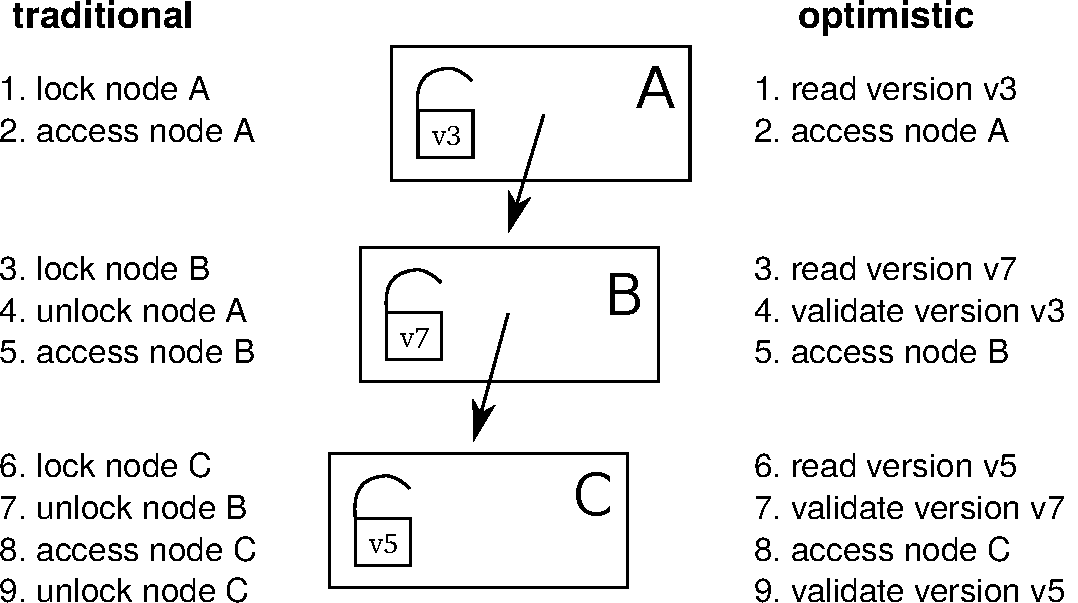
\includegraphics[width=0.65\linewidth]{olcall.pdf}
  \vspace{0.2cm}
  \caption{Comparison of a lookup operation in a 3-level tree using traditional lock coupling (left-hand side) vs.~optimistic lock coupling (right-hand side).}
  \label{fig:olc}
\end{figure}

The traditional and most common lock-based synchronization protocol for B-trees is lock coupling, which interleaves lock acquisitions while holding at most two locks at a time.
If, as we observed earlier, optimistic locks have similar semantics as traditional locks, it is natural to ask whether lock coupling can be combined with optimistic locks.
And indeed the answer is yes: One can almost mechanically translate traditional lock coupling code to optimistic lock coupling code.
This is illustrated in Figure~\ref{fig:olc}, which compares the traversal in a tree of height 3 using traditional and optimistic locks.
As the figure shows, the main difference is that locking is translated to reading the version and that unlocking becomes validation of the previously read version.
This simple change provides efficient lock-free tree traversal without the need to design a complex synchronization protocol.

It is important to emphasize the conceptual simplicity of OLC in comparison to data structures that use custom protocols like the Bw-tree~\cite{DBLP:conf/icde/LevandoskiLS13a}.
To implement lock-free access, the Bw-tree requires an indirection table, delta nodes, complex splitting and merging logic, retry logic, etc.
OLC, on the other hand, can directly be applied to B-trees mostly by adding the appropriate optimistic locking code and without modifying the node layout itself.
Therefore, OpenBw-Tree, an open source implementation of the Bw-tree, requires an order of magnitude more code than a B-tree based on OLC\footnote{Both implementations are available on GitHub: \url{https://github.com/wangziqi2016/index-microbench}}.
Given how difficult it is to develop, validate, and debug lock-free code, simplicity is obviously a major advantage.

\subsection{Correctness Aspects}

\begin{figure}
  % \centering
  %[basicstyle=\normalsize\ttfamily,showstringspaces=false,columns=fullflexible,breaklines=false,breakatwhitespace=true,numbers=none,numberstyle=\small,style=C,keepspaces=true]
\begin{lstlisting}[basicstyle=\ttfamily,language=C++,numbers=left,numberstyle=\small]
std::atomic<BTreeNode*> root;

// search for key in B+tree, returns payload in resultOut
bool lookup(Key key, Value& resultOut) {
   BTreeNode* node = root.load();
   uint64_t nodeVersion = node->readLockOrRestart();
   if (node != root.load()) // make sure the root is still the root
      restart();

   BTreeInner<Key>* parent = nullptr;
   uint64_t parentVersion = 0;

   while (node->isInner()) {
      auto inner = (BTreeInner*)node;

      // unlock parent and make current node the parent
      if (parent)
         parent->readUnlockOrRestart(parentVersion);
      parent = inner;
      parentVersion = nodeVersion;

      // search for next node
      node = inner->findChild(key);
      // validate 'inner' to ensure that 'node' pointer is valid
      inner->checkOrRestart(nodeVersion);
      // now it safe to dereference 'node' pointer (read its version)
      nodeVersion = node->readLockOrRestart();
   }

   // search in leaf and retrieve payload
   auto leaf = (BTreeLeaf*)node;
   bool success = leaf->findValue(key, resultOut);

   // unlock everything
   if (parent)
      parent->readUnlockOrRestart(parentVersion);
   node->readUnlockOrRestart(nodeVersion);

   return success;
}
\end{lstlisting}
  \vspace{0.2cm}
  \caption{B-tree lookup code using OLC. For simplicity, the restart logic is not shown.}
  \label{fig:lookup}
\end{figure}

So far, we have introduced the high-level ideas behind OLC and have stressed its similarity to traditional lock coupling.
Let us now discuss some cases where the close similarity between lock coupling and OLC breaks down.
To make this more concrete, we show the B-tree lookup code in Figure~\ref{fig:lookup}.
In the code, \texttt{readLockOrRestart} reads the lock version and \texttt{readUnlockOrRestart} validates that the read was correct.

One issue with OLC is that any pointer speculatively read from a node may point to invalid memory (if that node is modified concurrently).
Dereferencing such a pointer (e.g., to read its optimistic lock), may cause a segmentation fault or undefined behavior.
In the code shown in Figure~\ref{fig:lookup}, this problem is prevented by the extra check in line 25, which ensures that the read from the node containing the pointer was correct.
Without this additional validation, the code would in line 27 dereference the pointer speculatively read in line 23.
Note that the implementation of \texttt{checkOrRestart} is actually identical to \texttt{readUnlockOrRestart}.
We chose to give it a different name to highlight the fact that this extra check would not be necessary with read/write locks.

Another potential issue with optimistic locks is code that does not terminate.
Code that speculatively accesses a node, like an intra-node binary search, should be written in a way such that it always terminates---even in the presence of concurrent writes.
Otherwise, the validation code that detects the concurrent write will never run.
The binary search of a B-tree, for example, needs to be written in such a way that each comparison makes progress.
For some data structures that do not require loops in the traversal code (like ART) termination is trivially true.

\subsection{Implementation Details}

% implementation, efficiency
To implement an optimistic lock, one can combine the lock and the version counter into a single 64-bit\footnote{Even after subtracting one bit for the lock status, a back-of-the-envelope calculation can show that 63 bits are large enough to never overflow in practice.} word~\cite{artsync}.
A typical read operation will therefore merely consist of reading this version counter atomically.
In C++11 this can be implemented using the \texttt{std::atomic} type.

On x86, atomic reads are cheap because of x86's strong memory order guarantees.
No memory fences are required for sequentially-consistent loads, which are translated (by both GCC and clang) into standard \texttt{MOV} instructions.
Hence, the only effect of \texttt{std::atomic} for loads is preventing instruction re-ordering.
This makes version access and validation cheap.
Acquiring and releasing an optimistic lock in exclusive mode has comparable cost to a traditional lock:
A fairly expensive sequentially-consistent store is needed for acquiring a lock, while a standard \texttt{MOV} suffices for releasing it.
A simple sinlock-based implementation of optimistic locks can be found in the appendix of an earlier paper~\cite{artsync}.

OLC code must be able to handle restarts since validation or lock upgrade can fail due to concurrent writers.
Restarts can easily be implemented by wrapping the data structure operation in a loop (for simplicity not shown in Figure~\ref{fig:lookup}).
Such a loop also enables limiting the number of optimistic retry operations and falling back to pessimistic locking in cases of very heavy contention.
The ability to fall back to traditional locking is a major advantage of OLC in terms of robustness over lock-free approaches, which do not have this option.

In addition to the optimistic shared mode and the exclusive mode, optimistic locks also support a ``shared pessimistic'' mode, which physically acquires the lock in shared mode (allowing multiple concurrent readers but no writers).
This mode is useful for table (or range) scans that touch many tuples on a leaf page (which would otherwise easily abort).
Finally, let us mention that large range scans and table scans, should be broken up into several per-node traversals as is done in the LeanStore~\cite{leanstore} system.

Like all lock-free data structures, but unlike traditional locking and Hardware Transactional Memory~\cite{DBLP:conf/hpca/KarnagelDRLLSL14,DBLP:journals/pvldb/MakreshanskiLS15,htmtkde}, OLC requires care when deleting (and reusing) nodes.
The reason is that a deleting thread can never be sure that a node can be reclaimed because other threads might still be optimistically reading from that node.
Therefore, standard solutions like epoch-based reclamation~\cite{DBLP:conf/sosp/TuZKLM13}, hazard pointers~\cite{DBLP:journals/tpds/Michael04}, or optimized hazard pointers~\cite{DBLP:conf/spaa/BalmauGHZ16} need to be used.
These memory reclamation techniques are, however, largely orthogonal to the synchronization protocol itself.

%-lock-free is not a strong guarantee

\newpage
\section{Evaluation}\label{sec:evaluation}

Let us now experimentally evaluate the overhead and scalability of OLC.
For the experiments, we use an in-memory B+tree implemented in C++11 using templates, which is configured to use nodes of 4096 bytes, random 8 byte keys, and 8 byte payloads.
Based on this B-tree, we compare the following synchronization approaches:
\begin{itemize}
\item an OLC implementation\footnote{An almost identical OLC implementation is available on github: \url{https://github.com/wangziqi2016/index-microbench/tree/master/BTreeOLC}}
\item a variant based on traditional lock coupling and read/write locks
\item the unsynchronized B-tree, which obviously is only correct for read-only workloads but allows measuring the overhead of synchronization
\end{itemize}
Note that earlier work has compared the OLC implementation with a Bw-tree implementation~\cite{buzzword} and other state-of-the-art in-memory index structures.

We use a Haswell EP system with an Intel Xeon E5-2687W v3 CPU, which has 10 cores (20 ``Hyper-Threads'') and 25~MB of L3 cache.
The system is running Ubuntu 18.10 and we use GCC 8.2.0 to compile our code.
The CPU counters are obtained using the Linux perf API\footnote{We use the following convenience wrapper: \url{https://github.com/viktorleis/perfevent}}.

\begin{table}
  \caption{Performance and CPU counters for lookup and insert operations in a B-tree with 100M keys. We perform 100M operations and normalize the CPU counters by that number.}
  \label{tab:overhead}
  \centering
  \begin{tabular}{lrrrrrrr}\toprule
                    &         &        &        & instruc-  & L1     & L3     & branch \\
                    & threads & M op/s & cycles & tions & misses & misses & misses \\\midrule
lookup (no sync.)   & 1       & 1.72   & 2028   & 283     & 39.1   & 14.9   & 16.1   \\
lookup (OLC)        & 1       & 1.65   & 2107   & 370     & 43.9   & 15.1   & 16.7   \\
lookup (lock coup.) & 1       & 1.72   & 2078   & 365     & 42.3   & 16.9   & 15.7   \\\midrule
insert (no sync.)   & 1       & 1.51   & 2286   & 530     & 59.8   & 31.1   & 17.3   \\
insert (OLC)        & 1       & 1.50   & 2303   & 629     & 61.2   & 31.1   & 16.5   \\
insert (lock coup.) & 1       & 1.41   & 2473   & 644     & 61.0   & 31.0   & 17.2   \\\midrule
lookup (no sync.)   & 10      & 15.48  & 2058   & 283     & 38.6   & 15.5   & 16.0   \\
lookup (OLC)        & 10      & 14.60  & 2187   & 370     & 43.8   & 15.8   & 16.8   \\
lookup (lock coup.) & 10      & 5.71   & 5591   & 379     & 54.2   & 17.0   & 14.8   \\\midrule
insert (no sync.)   & 10      & -      & -      & -       & -      & -      & -      \\
insert (OLC)        & 10      & 10.46  & 2940   & 656     & 62.0   & 32.5   & 16.8   \\
insert (lock coup.) & 10      & 7.55   & 4161   & 667     & 75.0   & 28.6   & 16.2   \\
    \bottomrule
\end{tabular}
\end{table}

Table~\ref{tab:overhead} compares the performance and CPU counters for lookup and insert operations in a B-tree with 100M keys.
With {\em single-threaded} execution, we observe that all three approaches have very similar performance.
Adding traditional or optimistic locks to unsynchronized B-tree code results in up to 30\% of additional instructions without affecting single-threaded performance much.

\begin{figure}
  \centering
  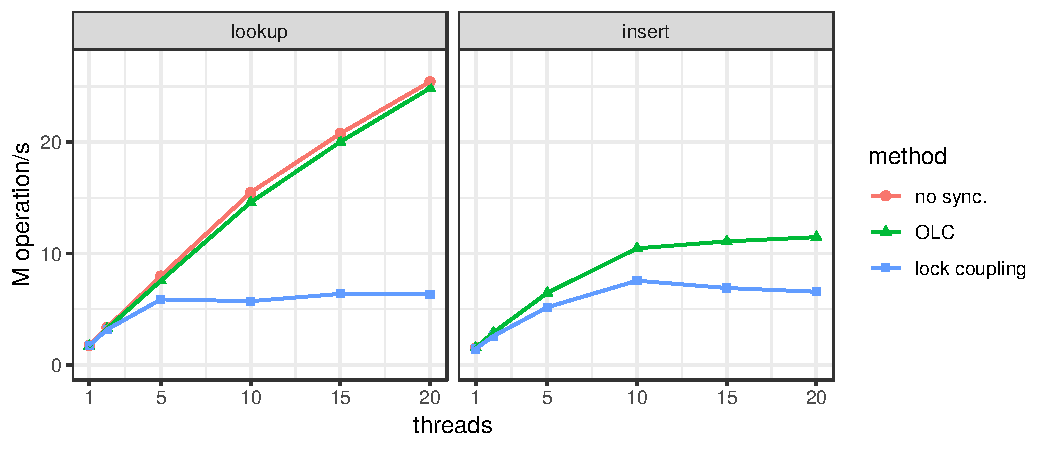
\includegraphics[width=\linewidth]{scale.pdf}
  \vspace{0.2cm}
  \caption{Scalability on 10-core system for B-tree operations (100M values).}
  \label{fig:scale}
\end{figure}

As Figure~\ref{fig:scale} shows, the results change dramatically once we use multiple threads.
For lookup, the scalability of OLC is near-linear up to 20 threads, even though the system has only 10 ``real cores''.
The OLC scalability for insert is also respectable (though not quite as linear because multi-threaded insertion approaches the memory bandwidth of our processor).
The figure also shows that the results of traditional lock coupling with read/write locks are significantly worse than OLC.
With 20 threads, lookup with OLC is 3.9$\times$ faster than traditional lock coupling.

\section{Summary}\label{sec:conc}

Optimistic Lock Coupling (OLC) is an effective synchronization method that combines the simplicity of traditional lock coupling with the superior scalability of lock-free approaches.
OLC is widely applicable and has already been successfully used to synchronize several data structures, including B-trees, binary search trees, and different trie variants.
These features make it highly attractive for modern database systems as well as performance-critical systems software in general.

\begin{thebibliography}{10}

\bibitem{DBLP:conf/spaa/BalmauGHZ16}
O.~Balmau, R.~Guerraoui, M.~Herlihy, and I.~Zablotchi.
\newblock Fast and robust memory reclamation for concurrent data structures.
\newblock In {\em SPAA}, 2016.

\bibitem{DBLP:journals/acta/BayerS77}
R.~Bayer and M.~Schkolnick.
\newblock Concurrency of operations on {B}-trees.
\newblock {\em Acta Informatica}, 9, 1977.

\bibitem{hot}
R.~Binna, E.~Zangerle, M.~Pichl, G.~Specht, and V.~Leis.
\newblock {HOT}: A height optimized trie index for main-memory database
  systems.
\newblock In {\em SIGMOD}, 2018.

\bibitem{DBLP:conf/ppopp/BronsonCCO10}
N.~G. Bronson, J.~Casper, H.~Chafi, and K.~Olukotun.
\newblock A practical concurrent binary search tree.
\newblock In {\em PPOPP}, 2010.

\bibitem{DBLP:conf/vldb/ChaHKK01}
S.~K. Cha, S.~Hwang, K.~Kim, and K.~Kwon.
\newblock Cache-conscious concurrency control of main-memory indexes on
  shared-memory multiprocessor systems.
\newblock In {\em VLDB}, 2001.

\bibitem{intel}
I.~Cutress.
\newblock {Intel} goes for 48-cores: {Cascade-AP} with multi-chip package
  coming soon.
\newblock
  \url{https://www.anandtech.com/show/13535/intel-goes-for-48cores-cascade-ap},
  2018 (accessed January, 2019).

\bibitem{DBLP:conf/cidr/FaleiroA17}
J.~M. Faleiro and D.~J. Abadi.
\newblock Latch-free synchronization in database systems: Silver bullet or
  fool's gold?
\newblock In {\em CIDR}, 2017.

\bibitem{DBLP:journals/ftdb/Graefe11}
G.~Graefe.
\newblock Modern {B}-tree techniques.
\newblock {\em Foundations and Trends in Databases}, 3(4), 2011.

\bibitem{DBLP:conf/hpca/KarnagelDRLLSL14}
T.~Karnagel, R.~Dementiev, R.~Rajwar, K.~Lai, T.~Legler, B.~Schlegel, and
  W.~Lehner.
\newblock Improving in-memory database index performance with
  {Intel}\({}^{\mbox{{\textregistered}}}\) transactional synchronization
  extensions.
\newblock In {\em HPCA}, 2014.

\bibitem{DBLP:journals/tods/LehmanY81}
P.~L. Lehman and S.~B. Yao.
\newblock Efficient locking for concurrent operations on {B}-trees.
\newblock {\em {ACM} Trans. Database Syst.}, 6(4), 1981.

\bibitem{leanstore}
V.~Leis, M.~Haubenschild, A.~Kemper, and T.~Neumann.
\newblock Leanstore: In-memory data management beyond main memory.
\newblock In {\em ICDE}, 2018.

\bibitem{art}
V.~Leis, A.~Kemper, and T.~Neumann.
\newblock The adaptive radix tree: {ARTful} indexing for main-memory databases.
\newblock In {\em ICDE}, 2013.

\bibitem{htmtkde}
V.~Leis, A.~Kemper, and T.~Neumann.
\newblock Scaling {HTM}-supported database transactions to many cores.
\newblock {\em {IEEE} Trans. Knowl. Data Eng.}, 28(2), 2016.

\bibitem{artsync}
V.~Leis, F.~Scheibner, A.~Kemper, and T.~Neumann.
\newblock The {ART} of practical synchronization.
\newblock In {\em DaMoN}, 2016.

\bibitem{DBLP:conf/icde/LevandoskiLS13a}
J.~J. Levandoski, D.~B. Lomet, and S.~Sengupta.
\newblock The {Bw}-tree: A {B}-tree for new hardware platforms.
\newblock In {\em ICDE}, 2013.

\bibitem{DBLP:journals/pvldb/MakreshanskiLS15}
D.~Makreshanski, J.~J. Levandoski, and R.~Stutsman.
\newblock To lock, swap, or elide: On the interplay of hardware transactional
  memory and lock-free indexing.
\newblock {\em {PVLDB}}, 8(11), 2015.

\bibitem{DBLP:dblp_conf/eurosys/MaoKM12}
Y.~Mao, E.~Kohler, and R.~T. Morris.
\newblock Cache craftiness for fast multicore key-value storage.
\newblock In {\em EuroSys}, 2012.

\bibitem{DBLP:journals/tpds/Michael04}
M.~M. Michael.
\newblock Hazard pointers: Safe memory reclamation for lock-free objects.
\newblock {\em {IEEE} Trans. Parallel Distrib. Syst.}, 15(6), 2004.

\bibitem{DBLP:journals/jacm/ShalevS06}
O.~Shalev and N.~Shavit.
\newblock Split-ordered lists: Lock-free extensible hash tables.
\newblock {\em J. {ACM}}, 53(3), 2006.

\bibitem{amd}
A.~Shilov.
\newblock {AMD} previews {EPYC} ‘{Rome}’ processor: Up to 64 {Zen} 2 cores.
\newblock
  \url{https://www.anandtech.com/show/13561/amd-previews-epyc-rome-processor-up-to-64-zen-2-cores},
  2018 (accessed January, 2019).

\bibitem{DBLP:conf/sosp/TuZKLM13}
S.~Tu, W.~Zheng, E.~Kohler, B.~Liskov, and S.~Madden.
\newblock Speedy transactions in multicore in-memory databases.
\newblock In {\em SOSP}, 2013.

\bibitem{buzzword}
Z.~Wang, A.~Pavlo, H.~Lim, V.~Leis, H.~Zhang, M.~Kaminsky, and D.~Andersen.
\newblock Building a {Bw}-tree takes more than just buzz words.
\newblock In {\em SIGMOD}, 2018.

\end{thebibliography}


%\bibliographystyle{abbrv}
%\bibliography{main}

\end{document}

\end{article}

\begin{article}
{Experiences in Exascale Scientific Data Management}
{Mario Lassnig, Martin Barisits and Dimitrios Christidis}
\graphicspath{{submissions/mario/}}
\pdfminorversion=5
\documentclass[11pt]{article}
\usepackage{deauthor,times,graphicx,caption,microtype}
\usepackage{hyperref}
\usepackage{listings}
\usepackage{booktabs}

\begin{document}

\title{Optimistic Lock Coupling: A Scalable and Efficient General-Purpose Synchronization Method}

\author{Viktor Leis, Michael Haubenschild\raisebox{0.9ex}{$\ast$}, Thomas Neumann\\ Technische Universit{\"a}t M{\"u}nchen \hspace{0.7cm} Tableau Software\raisebox{0.9ex}{$\ast$} \\ {\{leis,neumann\}{@}in.tum.de} \hspace{0.7cm} {mhaubenschild{@}tableau.com\raisebox{0.9ex}{$\ast$}}}

\maketitle

\begin{abstract}
As the number of cores on commodity processors continues to increase, scalability becomes more and more crucial for overall performance.
Scalable and efficient concurrent data structures are particularly important, as these are often the building blocks of parallel algorithms.
Unfortunately, traditional synchronization techniques based on fine-grained locking have been shown to be unscalable on modern multi-core CPUs.
Lock-free data structures, on the other hand, are extremely difficult to design and often incur significant overhead.

In this work, we make the case for Optimistic Lock Coupling as a practical alternative to both traditional locking and the lock-free approach.
We show that Optimistic Lock Coupling is highly scalable and almost as simple to implement as traditional lock coupling.
Another important advantage is that it is easily applicable to most tree-like data structures.
We therefore argue that Optimistic Lock Coupling, rather than a complex and error-prone custom synchronization protocol, should be the default choice for performance-critical data structures.
\end{abstract}

\section{Introduction}

% more and more cores
Today, Intel's commodity server processors have up to 28 cores and its upcoming microarchitecture will have up to 48 cores per socket~\cite{intel}.
Similarly, AMD currently stands at 32 cores and this number is expected to double in the next generation~\cite{amd}.
Since both platforms support simultaneous multithreading (also known as hyperthreading), affordable commodity servers (with up to two sockets) will soon routinely have between 100 and 200 hardware threads.

% data structure scalability is important
With such a high degree of hardware parallelism, efficient data processing crucially depends on how well concurrent data structures scale.
Internally, database systems use a plethora of data structures like table heaps, internal work queues, and, most importantly, index structures.
Any of these can easily become a scalability (and therefore overall performance) bottleneck on many-core CPUs.

% traditional synchronization: fine-grained locks, slow, cache invalidation
Traditionally, database systems synchronize internal data structures using fine-grained reader/writer locks\footnote{In this work, we focus on data structure synchronization rather than high-level transaction semantics and therefore use the term {\em lock} for what would typically be called {\em latch} in the database literature. We thus follow common computer science (rather than database) terminology.}.
Unfortunately, while fine-grained locking makes lock contention unlikely, it still results in bad scalability because lock acquisition and release require writing to shared memory.
Due to the way cache coherency is implemented on modern multi-core CPUs, these writes cause additional cache misses\footnote{The cache coherency protocol ensures that all copies of a cache line on other cores are invalidated before the write can proceed.} and the cache line containing the lock's internal data becomes a point of physical contention.
As a result, any frequently-accessed lock (e.g., the lock of the root node of a B-tree) severely limits scalability.

% lock-free bw-tree: no more latches, but indirections, extremely complex
Lock-free data structures like the Bw-tree~\cite{DBLP:conf/icde/LevandoskiLS13a} (a lock-free B-tree variant) or the Split-Ordered List~\cite{DBLP:journals/jacm/ShalevS06} (a lock-free hash table) do not acquire any locks and therefore generally scale much better than locking-based approaches (in particular for read-mostly workloads).
However, lock-free synchronization has other downsides:
First, it is very difficult and results in extremely complex and error-prone code (when compared to locking).
Second, because the functionality of atomic primitives provided by the hardware (e.g., atomically compare-and-swap 8 bytes) is limited, complex operations require additional indirections within the data structure.
For example, the Bw-tree requires an indirection table and the Split-Ordered List requires ``dummy nodes'', resulting in overhead due to additional cache misses.

% OLC for the win
In this paper we make the case for {\em Optimistic Lock Coupling (OLC)}, a synchronization method that combines some of the best properties of lock-based and lock-free synchronization.
OLC utilizes a special lock type that can be used in two modes:
The first mode is similar to a traditional mutex and excludes other threads by physically acquiring the underlying lock.
In the second mode, reads can proceed optimistically by validating a version counter that is embedded in the lock (similar to optimistic concurrency control).
The first mode is typically used by writers and the second mode by readers.
Besides this special lock type, OLC is based on the observation that optimistic lock validations can be interleaved/coupled---similar to the pair-wise interleaved lock acquisition of traditional lock coupling.
Hence, the name Optimistic Lock Coupling.

OLC has a number of desirable features:
\begin{itemize}
\item By reducing the number of writes to shared memory locations and thereby avoiding cache invalidations, it {\bf scales well} for most workloads.
\item In comparison to unsynchronized code, it requires few additional CPU instructions making it {\bf efficient}.
\item OLC is {\bf widely applicable} to different data structures. It has already been successfully used for synchronizing binary search trees~\cite{DBLP:conf/ppopp/BronsonCCO10}, tries~\cite{artsync}, trie/B-tree hybrids~\cite{DBLP:dblp_conf/eurosys/MaoKM12}, and B-trees~\cite{buzzword}.
\item In comparison to the lock-free paradigm, it is also {\bf easy to use} and requires few modifications to existing, single-threaded data structures.
\end{itemize}
Despite these positive features and its simplicity, OLC is not yet widely known.
The goal of this paper is therefore to popularize this simple idea and to make a case for it.
We argue that OLC deserves to be widely known.
It is a good default synchronization paradigm---more complex, data structure-specific protocols are seldom beneficial.

The rest of the paper is organized as follows.
Section~\ref{sec:related} discusses related work, tracing the history of OLC and its underlying ideas in the literature.
The core of the paper is Section~\ref{sec:olc}, which describes the ideas behind OLC and how it can be used to synchronize complex data structures.
In Section~\ref{sec:evaluation} we experimentally show that OLC has low overhead and scales well when used to synchronize an in-memory B-tree.
We summarize the paper in Section~\ref{sec:conc}.

\newpage
\section{Related Work}\label{sec:related}

Lock coupling has been proposed as a method for allowing concurrent operations on B-trees in 1977~\cite{DBLP:journals/acta/BayerS77}.
This traditional and still widely-used method, described in detail in Graefe's B-tree survey~\cite{DBLP:journals/ftdb/Graefe11}, is also called ``latch coupling'', ``hand-over-hand locking'', and ``crabbing''.
Because at most two locks are held at-a-time during tree traversal, this technique seemingly allows for a high degree of parallelism---in particular if read/write locks are used to enable inner nodes to be locked in shared mode.
However, as we show in Section~\ref{sec:evaluation}, on modern hardware lock acquisition (even in shared mode) results in suboptimal scalability.

An early alternative from 1981 is a B-tree variant called B-link tree~\cite{DBLP:journals/tods/LehmanY81}, which only holds a single lock at a time.
It is based on the observation that between the release of the parent lock and the acquisition of the child lock, the only ``dangerous'' thing that could have happened is the split of a child node (assuming one does not implement merge operations).
Thus, when a split happens, the key being searched might end up on a neighboring node to the right of the current child node.
A B-link tree traversal therefore detects this condition and, if needed, transparently proceeds to the neighboring node.
Releasing the parent lock early is highly beneficial when the child node needs to be fetched from disk.
For in-memory workloads, however, the B-link tree has the same scalability issues as lock coupling (it acquires just as many locks).

The next major advance, Optimistic Latch-Free Index Traversal (OLFIT)~\cite{DBLP:conf/vldb/ChaHKK01}, was proposed in 2001.
OLFIT introduced the idea of a combined lock/update counter, which we call {\em optimistic lock}. % , for lack of a better name,
Based on these per-node optimistic locks and the synchronization protocol of the B-link tree, OLFIT finally achieves good scalability on parallel processors.
The OLFIT protocol is fairly complex, as it requires both the non-trivial B-link protocol and optimistic locks.
Furthermore, like the B-link tree protocol, it does not support merging nodes, and is specific to B-trees (cannot easily be applied to other data structures).

In the following two decades, the growth of main-memory capacity led to much research into other data structures besides the venerable B-tree.
Particularly relevant for our discussion is Bronson et al.'s~\cite{DBLP:conf/ppopp/BronsonCCO10} concurrent binary search tree, which is based on optimistic version validation and has a sophisticated, data structure-specific synchronization protocol.
To the best of our knowledge, this 2010 paper is the first that, as part of its protocol, interleaves version validation across nodes---rather than validating each node separately like OLFIT.
In that paper, this idea is called ``hand-over-hand, optimistic validation'', while we prefer the term Optimistic Lock Coupling to highlight the close resemblance to traditional lock coupling.
Similarly, Mao et al.'s~\cite{DBLP:dblp_conf/eurosys/MaoKM12} Masstree (a concurrent hybrid trie/B-tree) is also based on the same ideas, but again uses them as part of a more complex protocol.

The Adaptive Radix Tree (ART)~\cite{art} is another recent in-memory data structure, which we proposed in 2013.
In contrast to the two data structures just mentioned, it was originally designed with single-threaded performance in mind without supporting concurrency.
To add support for concurrency, we initially started designing a custom protocol called Read-Optimized Write Exclusion (ROWEX)~\cite{artsync}, which turned out to be non-trivial and requires modifications of the underlying data structure\footnote{Note that ROWEX is already easier to apply to existing data structures than the lock-free approach. The difficulty depends on the data structure. Applying ROWEX is hard for B-trees with sorted keys and fairly easy for copy-on-write data structures like the Height Optimized Trie~\cite{hot}---with ART being somewhere in the middle.}.
However, fairly late in the project, we also realized, that OLC {\em alone} (rather than as part of a more complex protocol) is sufficient to synchronize ART.
No other changes to the data structure were necessary.
Both approaches were published and experimentally evaluated in a followup paper~\cite{artsync}, which shows that, despite its simplicity, OLC is efficient, scalable, and generally outperforms ROWEX.

Similar results were recently published regarding B-trees~\cite{buzzword}.
In this experimental study a simple OLC-based synchronization outperformed the Bw-tree~\cite{DBLP:conf/icde/LevandoskiLS13a}, a complex lock-free synchronization approach.
Another recent paper shows that for write-intensive workloads, locking often performs better than lock-free synchronization~\cite{DBLP:conf/cidr/FaleiroA17}.
These experiences indicate that OLC is a general-purpose synchronization paradigm and motivate the current paper.

%foster b-tree\cite{DBLP:journals/tods/GraefeKK12}
%Shasha theory~\cite{DBLP:journals/tods/ShashaG88}

\section{Optimistic Lock Coupling}\label{sec:olc}

% locks suck
The standard technique for inter-thread synchronization is mutual exclusion using fine-grained locks.
In a B-tree, for example, every node usually has its own associated lock, which is acquired before accessing that node.
The problem of locking on modern multi- and many-core processors is that lock acquisition and release require writing to the shared memory location that implements the lock.
This write causes exclusive ownership of the underlying cache line and invalidates copies of it on all other processor cores.
For hierarchical, tree-like data structures, the lock of the root node becomes a point of physical contention---even in read-only workloads and even when read/write locks are used.
Depending on the specific data structure, number of cores, cache coherency protocol implementation, cache topology, whether Non-Uniform Memory Access (NUMA) is used, locking can even result in multi-threaded performance that is worse than single-threaded execution.

% in b-trees this happens very much
The inherent pessimism of locking is particularly unfortunate for B-trees:
Despite the fact that logical modifications of the root node are very infrequent, every B-tree operation must lock the root node during tree traversal\footnote{To a lesser extent this obviously applies to all inner nodes, not just the root.}.
Even the vast majority of update operations (with the exception of splits and merges), only modify a single leaf node.
These observations indicate that a more optimistic approach, which does not require locking inner nodes, would be very beneficial for B-trees.

\subsection{Optimistic Locks}

% optimism to the rescue
As the name indicates, optimistic locks try to solve the scalability issues of traditional locks using an optimistic approach.
Instead of always physically acquiring locks, even for nodes that are unlikely to be modified simultaneously, after-the-fact validation is used to detect conflicts.
This is done by augmenting each lock with a version/update counter that is incremented on every modification.
Using this version counter, readers can optimistically proceed before validating that the version did not change to ensure that the read was safe.
If validation fails, the operation is restarted.

% details on opt locks
Using optimistic locks, a read-only node access (i.e., the majority of all operations in a B-tree) does not acquire the lock and does not increment the version counter.
Instead, it performs the following steps:
\begin{enumerate}
\item read lock version (restart if lock is not free)
\item access node
\item read the version again and validate that it has not changed in the meantime
\end{enumerate}
If the last step (the validation) fails, the operation has to be restarted.
Write operations, on the other hand, are more similar to traditional locking:
\begin{enumerate}
\item acquire lock (wait if necessary)
\item access/write to node
\item increment version and unlock node
\end{enumerate}
Writes can therefore protect a node from other writes.

% similar to locks
As we observed in an earlier paper~\cite{artsync}, because of similar semantics, optimistic locks can be hidden behind an API very similar to traditional read/write locks.
Both approaches have an exclusive lock mode, and acquiring a traditional lock in shared mode is analogous to optimistic version validation.
Furthermore, like with some implementations of traditional read/write locks, optimistic locks allow upgrading a shared lock to an exclusive lock.
Lock upgrades are, for example, used to avoid most B-tree update operations from having to lock inner nodes.
In our experience, the close resemblance of optimistic and traditional locks simplifies the reasoning about optimistic locks;
one can apply similar thinking as in traditional lock-based protocols.

\subsection{Lock Coupling with Optimistic Locks}

\begin{figure}
  \centering
  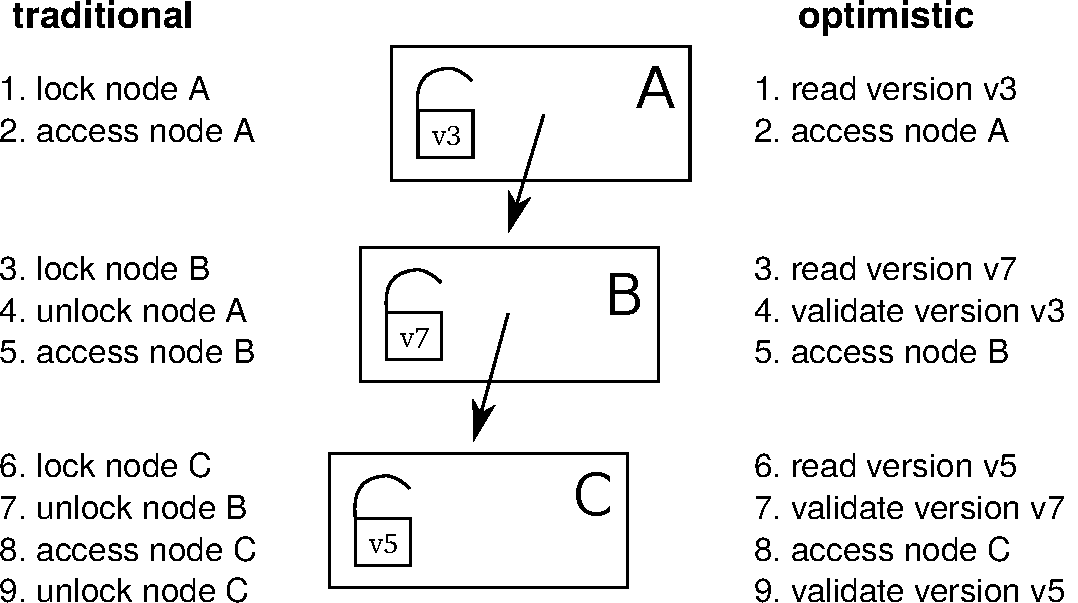
\includegraphics[width=0.65\linewidth]{olcall.pdf}
  \vspace{0.2cm}
  \caption{Comparison of a lookup operation in a 3-level tree using traditional lock coupling (left-hand side) vs.~optimistic lock coupling (right-hand side).}
  \label{fig:olc}
\end{figure}

The traditional and most common lock-based synchronization protocol for B-trees is lock coupling, which interleaves lock acquisitions while holding at most two locks at a time.
If, as we observed earlier, optimistic locks have similar semantics as traditional locks, it is natural to ask whether lock coupling can be combined with optimistic locks.
And indeed the answer is yes: One can almost mechanically translate traditional lock coupling code to optimistic lock coupling code.
This is illustrated in Figure~\ref{fig:olc}, which compares the traversal in a tree of height 3 using traditional and optimistic locks.
As the figure shows, the main difference is that locking is translated to reading the version and that unlocking becomes validation of the previously read version.
This simple change provides efficient lock-free tree traversal without the need to design a complex synchronization protocol.

It is important to emphasize the conceptual simplicity of OLC in comparison to data structures that use custom protocols like the Bw-tree~\cite{DBLP:conf/icde/LevandoskiLS13a}.
To implement lock-free access, the Bw-tree requires an indirection table, delta nodes, complex splitting and merging logic, retry logic, etc.
OLC, on the other hand, can directly be applied to B-trees mostly by adding the appropriate optimistic locking code and without modifying the node layout itself.
Therefore, OpenBw-Tree, an open source implementation of the Bw-tree, requires an order of magnitude more code than a B-tree based on OLC\footnote{Both implementations are available on GitHub: \url{https://github.com/wangziqi2016/index-microbench}}.
Given how difficult it is to develop, validate, and debug lock-free code, simplicity is obviously a major advantage.

\subsection{Correctness Aspects}

\begin{figure}
  % \centering
  %[basicstyle=\normalsize\ttfamily,showstringspaces=false,columns=fullflexible,breaklines=false,breakatwhitespace=true,numbers=none,numberstyle=\small,style=C,keepspaces=true]
\begin{lstlisting}[basicstyle=\ttfamily,language=C++,numbers=left,numberstyle=\small]
std::atomic<BTreeNode*> root;

// search for key in B+tree, returns payload in resultOut
bool lookup(Key key, Value& resultOut) {
   BTreeNode* node = root.load();
   uint64_t nodeVersion = node->readLockOrRestart();
   if (node != root.load()) // make sure the root is still the root
      restart();

   BTreeInner<Key>* parent = nullptr;
   uint64_t parentVersion = 0;

   while (node->isInner()) {
      auto inner = (BTreeInner*)node;

      // unlock parent and make current node the parent
      if (parent)
         parent->readUnlockOrRestart(parentVersion);
      parent = inner;
      parentVersion = nodeVersion;

      // search for next node
      node = inner->findChild(key);
      // validate 'inner' to ensure that 'node' pointer is valid
      inner->checkOrRestart(nodeVersion);
      // now it safe to dereference 'node' pointer (read its version)
      nodeVersion = node->readLockOrRestart();
   }

   // search in leaf and retrieve payload
   auto leaf = (BTreeLeaf*)node;
   bool success = leaf->findValue(key, resultOut);

   // unlock everything
   if (parent)
      parent->readUnlockOrRestart(parentVersion);
   node->readUnlockOrRestart(nodeVersion);

   return success;
}
\end{lstlisting}
  \vspace{0.2cm}
  \caption{B-tree lookup code using OLC. For simplicity, the restart logic is not shown.}
  \label{fig:lookup}
\end{figure}

So far, we have introduced the high-level ideas behind OLC and have stressed its similarity to traditional lock coupling.
Let us now discuss some cases where the close similarity between lock coupling and OLC breaks down.
To make this more concrete, we show the B-tree lookup code in Figure~\ref{fig:lookup}.
In the code, \texttt{readLockOrRestart} reads the lock version and \texttt{readUnlockOrRestart} validates that the read was correct.

One issue with OLC is that any pointer speculatively read from a node may point to invalid memory (if that node is modified concurrently).
Dereferencing such a pointer (e.g., to read its optimistic lock), may cause a segmentation fault or undefined behavior.
In the code shown in Figure~\ref{fig:lookup}, this problem is prevented by the extra check in line 25, which ensures that the read from the node containing the pointer was correct.
Without this additional validation, the code would in line 27 dereference the pointer speculatively read in line 23.
Note that the implementation of \texttt{checkOrRestart} is actually identical to \texttt{readUnlockOrRestart}.
We chose to give it a different name to highlight the fact that this extra check would not be necessary with read/write locks.

Another potential issue with optimistic locks is code that does not terminate.
Code that speculatively accesses a node, like an intra-node binary search, should be written in a way such that it always terminates---even in the presence of concurrent writes.
Otherwise, the validation code that detects the concurrent write will never run.
The binary search of a B-tree, for example, needs to be written in such a way that each comparison makes progress.
For some data structures that do not require loops in the traversal code (like ART) termination is trivially true.

\subsection{Implementation Details}

% implementation, efficiency
To implement an optimistic lock, one can combine the lock and the version counter into a single 64-bit\footnote{Even after subtracting one bit for the lock status, a back-of-the-envelope calculation can show that 63 bits are large enough to never overflow in practice.} word~\cite{artsync}.
A typical read operation will therefore merely consist of reading this version counter atomically.
In C++11 this can be implemented using the \texttt{std::atomic} type.

On x86, atomic reads are cheap because of x86's strong memory order guarantees.
No memory fences are required for sequentially-consistent loads, which are translated (by both GCC and clang) into standard \texttt{MOV} instructions.
Hence, the only effect of \texttt{std::atomic} for loads is preventing instruction re-ordering.
This makes version access and validation cheap.
Acquiring and releasing an optimistic lock in exclusive mode has comparable cost to a traditional lock:
A fairly expensive sequentially-consistent store is needed for acquiring a lock, while a standard \texttt{MOV} suffices for releasing it.
A simple sinlock-based implementation of optimistic locks can be found in the appendix of an earlier paper~\cite{artsync}.

OLC code must be able to handle restarts since validation or lock upgrade can fail due to concurrent writers.
Restarts can easily be implemented by wrapping the data structure operation in a loop (for simplicity not shown in Figure~\ref{fig:lookup}).
Such a loop also enables limiting the number of optimistic retry operations and falling back to pessimistic locking in cases of very heavy contention.
The ability to fall back to traditional locking is a major advantage of OLC in terms of robustness over lock-free approaches, which do not have this option.

In addition to the optimistic shared mode and the exclusive mode, optimistic locks also support a ``shared pessimistic'' mode, which physically acquires the lock in shared mode (allowing multiple concurrent readers but no writers).
This mode is useful for table (or range) scans that touch many tuples on a leaf page (which would otherwise easily abort).
Finally, let us mention that large range scans and table scans, should be broken up into several per-node traversals as is done in the LeanStore~\cite{leanstore} system.

Like all lock-free data structures, but unlike traditional locking and Hardware Transactional Memory~\cite{DBLP:conf/hpca/KarnagelDRLLSL14,DBLP:journals/pvldb/MakreshanskiLS15,htmtkde}, OLC requires care when deleting (and reusing) nodes.
The reason is that a deleting thread can never be sure that a node can be reclaimed because other threads might still be optimistically reading from that node.
Therefore, standard solutions like epoch-based reclamation~\cite{DBLP:conf/sosp/TuZKLM13}, hazard pointers~\cite{DBLP:journals/tpds/Michael04}, or optimized hazard pointers~\cite{DBLP:conf/spaa/BalmauGHZ16} need to be used.
These memory reclamation techniques are, however, largely orthogonal to the synchronization protocol itself.

%-lock-free is not a strong guarantee

\newpage
\section{Evaluation}\label{sec:evaluation}

Let us now experimentally evaluate the overhead and scalability of OLC.
For the experiments, we use an in-memory B+tree implemented in C++11 using templates, which is configured to use nodes of 4096 bytes, random 8 byte keys, and 8 byte payloads.
Based on this B-tree, we compare the following synchronization approaches:
\begin{itemize}
\item an OLC implementation\footnote{An almost identical OLC implementation is available on github: \url{https://github.com/wangziqi2016/index-microbench/tree/master/BTreeOLC}}
\item a variant based on traditional lock coupling and read/write locks
\item the unsynchronized B-tree, which obviously is only correct for read-only workloads but allows measuring the overhead of synchronization
\end{itemize}
Note that earlier work has compared the OLC implementation with a Bw-tree implementation~\cite{buzzword} and other state-of-the-art in-memory index structures.

We use a Haswell EP system with an Intel Xeon E5-2687W v3 CPU, which has 10 cores (20 ``Hyper-Threads'') and 25~MB of L3 cache.
The system is running Ubuntu 18.10 and we use GCC 8.2.0 to compile our code.
The CPU counters are obtained using the Linux perf API\footnote{We use the following convenience wrapper: \url{https://github.com/viktorleis/perfevent}}.

\begin{table}
  \caption{Performance and CPU counters for lookup and insert operations in a B-tree with 100M keys. We perform 100M operations and normalize the CPU counters by that number.}
  \label{tab:overhead}
  \centering
  \begin{tabular}{lrrrrrrr}\toprule
                    &         &        &        & instruc-  & L1     & L3     & branch \\
                    & threads & M op/s & cycles & tions & misses & misses & misses \\\midrule
lookup (no sync.)   & 1       & 1.72   & 2028   & 283     & 39.1   & 14.9   & 16.1   \\
lookup (OLC)        & 1       & 1.65   & 2107   & 370     & 43.9   & 15.1   & 16.7   \\
lookup (lock coup.) & 1       & 1.72   & 2078   & 365     & 42.3   & 16.9   & 15.7   \\\midrule
insert (no sync.)   & 1       & 1.51   & 2286   & 530     & 59.8   & 31.1   & 17.3   \\
insert (OLC)        & 1       & 1.50   & 2303   & 629     & 61.2   & 31.1   & 16.5   \\
insert (lock coup.) & 1       & 1.41   & 2473   & 644     & 61.0   & 31.0   & 17.2   \\\midrule
lookup (no sync.)   & 10      & 15.48  & 2058   & 283     & 38.6   & 15.5   & 16.0   \\
lookup (OLC)        & 10      & 14.60  & 2187   & 370     & 43.8   & 15.8   & 16.8   \\
lookup (lock coup.) & 10      & 5.71   & 5591   & 379     & 54.2   & 17.0   & 14.8   \\\midrule
insert (no sync.)   & 10      & -      & -      & -       & -      & -      & -      \\
insert (OLC)        & 10      & 10.46  & 2940   & 656     & 62.0   & 32.5   & 16.8   \\
insert (lock coup.) & 10      & 7.55   & 4161   & 667     & 75.0   & 28.6   & 16.2   \\
    \bottomrule
\end{tabular}
\end{table}

Table~\ref{tab:overhead} compares the performance and CPU counters for lookup and insert operations in a B-tree with 100M keys.
With {\em single-threaded} execution, we observe that all three approaches have very similar performance.
Adding traditional or optimistic locks to unsynchronized B-tree code results in up to 30\% of additional instructions without affecting single-threaded performance much.

\begin{figure}
  \centering
  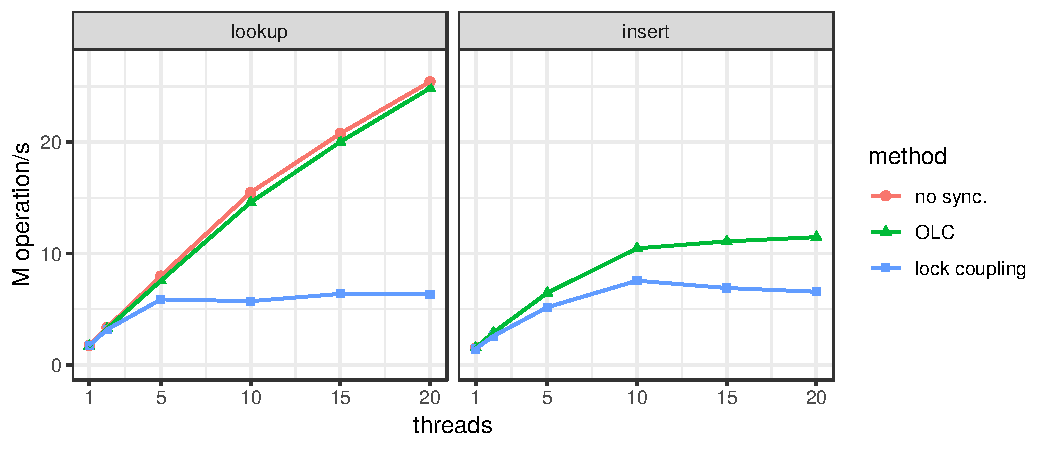
\includegraphics[width=\linewidth]{scale.pdf}
  \vspace{0.2cm}
  \caption{Scalability on 10-core system for B-tree operations (100M values).}
  \label{fig:scale}
\end{figure}

As Figure~\ref{fig:scale} shows, the results change dramatically once we use multiple threads.
For lookup, the scalability of OLC is near-linear up to 20 threads, even though the system has only 10 ``real cores''.
The OLC scalability for insert is also respectable (though not quite as linear because multi-threaded insertion approaches the memory bandwidth of our processor).
The figure also shows that the results of traditional lock coupling with read/write locks are significantly worse than OLC.
With 20 threads, lookup with OLC is 3.9$\times$ faster than traditional lock coupling.

\section{Summary}\label{sec:conc}

Optimistic Lock Coupling (OLC) is an effective synchronization method that combines the simplicity of traditional lock coupling with the superior scalability of lock-free approaches.
OLC is widely applicable and has already been successfully used to synchronize several data structures, including B-trees, binary search trees, and different trie variants.
These features make it highly attractive for modern database systems as well as performance-critical systems software in general.

\begin{thebibliography}{10}

\bibitem{DBLP:conf/spaa/BalmauGHZ16}
O.~Balmau, R.~Guerraoui, M.~Herlihy, and I.~Zablotchi.
\newblock Fast and robust memory reclamation for concurrent data structures.
\newblock In {\em SPAA}, 2016.

\bibitem{DBLP:journals/acta/BayerS77}
R.~Bayer and M.~Schkolnick.
\newblock Concurrency of operations on {B}-trees.
\newblock {\em Acta Informatica}, 9, 1977.

\bibitem{hot}
R.~Binna, E.~Zangerle, M.~Pichl, G.~Specht, and V.~Leis.
\newblock {HOT}: A height optimized trie index for main-memory database
  systems.
\newblock In {\em SIGMOD}, 2018.

\bibitem{DBLP:conf/ppopp/BronsonCCO10}
N.~G. Bronson, J.~Casper, H.~Chafi, and K.~Olukotun.
\newblock A practical concurrent binary search tree.
\newblock In {\em PPOPP}, 2010.

\bibitem{DBLP:conf/vldb/ChaHKK01}
S.~K. Cha, S.~Hwang, K.~Kim, and K.~Kwon.
\newblock Cache-conscious concurrency control of main-memory indexes on
  shared-memory multiprocessor systems.
\newblock In {\em VLDB}, 2001.

\bibitem{intel}
I.~Cutress.
\newblock {Intel} goes for 48-cores: {Cascade-AP} with multi-chip package
  coming soon.
\newblock
  \url{https://www.anandtech.com/show/13535/intel-goes-for-48cores-cascade-ap},
  2018 (accessed January, 2019).

\bibitem{DBLP:conf/cidr/FaleiroA17}
J.~M. Faleiro and D.~J. Abadi.
\newblock Latch-free synchronization in database systems: Silver bullet or
  fool's gold?
\newblock In {\em CIDR}, 2017.

\bibitem{DBLP:journals/ftdb/Graefe11}
G.~Graefe.
\newblock Modern {B}-tree techniques.
\newblock {\em Foundations and Trends in Databases}, 3(4), 2011.

\bibitem{DBLP:conf/hpca/KarnagelDRLLSL14}
T.~Karnagel, R.~Dementiev, R.~Rajwar, K.~Lai, T.~Legler, B.~Schlegel, and
  W.~Lehner.
\newblock Improving in-memory database index performance with
  {Intel}\({}^{\mbox{{\textregistered}}}\) transactional synchronization
  extensions.
\newblock In {\em HPCA}, 2014.

\bibitem{DBLP:journals/tods/LehmanY81}
P.~L. Lehman and S.~B. Yao.
\newblock Efficient locking for concurrent operations on {B}-trees.
\newblock {\em {ACM} Trans. Database Syst.}, 6(4), 1981.

\bibitem{leanstore}
V.~Leis, M.~Haubenschild, A.~Kemper, and T.~Neumann.
\newblock Leanstore: In-memory data management beyond main memory.
\newblock In {\em ICDE}, 2018.

\bibitem{art}
V.~Leis, A.~Kemper, and T.~Neumann.
\newblock The adaptive radix tree: {ARTful} indexing for main-memory databases.
\newblock In {\em ICDE}, 2013.

\bibitem{htmtkde}
V.~Leis, A.~Kemper, and T.~Neumann.
\newblock Scaling {HTM}-supported database transactions to many cores.
\newblock {\em {IEEE} Trans. Knowl. Data Eng.}, 28(2), 2016.

\bibitem{artsync}
V.~Leis, F.~Scheibner, A.~Kemper, and T.~Neumann.
\newblock The {ART} of practical synchronization.
\newblock In {\em DaMoN}, 2016.

\bibitem{DBLP:conf/icde/LevandoskiLS13a}
J.~J. Levandoski, D.~B. Lomet, and S.~Sengupta.
\newblock The {Bw}-tree: A {B}-tree for new hardware platforms.
\newblock In {\em ICDE}, 2013.

\bibitem{DBLP:journals/pvldb/MakreshanskiLS15}
D.~Makreshanski, J.~J. Levandoski, and R.~Stutsman.
\newblock To lock, swap, or elide: On the interplay of hardware transactional
  memory and lock-free indexing.
\newblock {\em {PVLDB}}, 8(11), 2015.

\bibitem{DBLP:dblp_conf/eurosys/MaoKM12}
Y.~Mao, E.~Kohler, and R.~T. Morris.
\newblock Cache craftiness for fast multicore key-value storage.
\newblock In {\em EuroSys}, 2012.

\bibitem{DBLP:journals/tpds/Michael04}
M.~M. Michael.
\newblock Hazard pointers: Safe memory reclamation for lock-free objects.
\newblock {\em {IEEE} Trans. Parallel Distrib. Syst.}, 15(6), 2004.

\bibitem{DBLP:journals/jacm/ShalevS06}
O.~Shalev and N.~Shavit.
\newblock Split-ordered lists: Lock-free extensible hash tables.
\newblock {\em J. {ACM}}, 53(3), 2006.

\bibitem{amd}
A.~Shilov.
\newblock {AMD} previews {EPYC} ‘{Rome}’ processor: Up to 64 {Zen} 2 cores.
\newblock
  \url{https://www.anandtech.com/show/13561/amd-previews-epyc-rome-processor-up-to-64-zen-2-cores},
  2018 (accessed January, 2019).

\bibitem{DBLP:conf/sosp/TuZKLM13}
S.~Tu, W.~Zheng, E.~Kohler, B.~Liskov, and S.~Madden.
\newblock Speedy transactions in multicore in-memory databases.
\newblock In {\em SOSP}, 2013.

\bibitem{buzzword}
Z.~Wang, A.~Pavlo, H.~Lim, V.~Leis, H.~Zhang, M.~Kaminsky, and D.~Andersen.
\newblock Building a {Bw}-tree takes more than just buzz words.
\newblock In {\em SIGMOD}, 2018.

\end{thebibliography}


%\bibliographystyle{abbrv}
%\bibliography{main}

\end{document}

\end{article}

\begin{article}
{$SUQ^{2}$: Uncertainty Quantification Queries over LargeSpatio-temporal Simulations}
{Noel Moreno Lemus, Fabio Porto, Yania M. Souto, Rafael S. Pereira, Ji Liu, Esther Pacciti, and Patrick Valduriez}
\graphicspath{{submissions/fabio/}}
%% 
%% Copyright 2007, 2008, 2009 Elsevier Ltd
%% 
%% This file is part of the 'Elsarticle Bundle'.
%% ---------------------------------------------
%% 
%% It may be distributed under the conditions of the LaTeX Project Public
%% License, either version 1.2 of this license or (at your option) any
%% later version.  The latest version of this license is in
%%    http://www.latex-project.org/lppl.txt
%% and version 1.2 or later is part of all distributions of LaTeX
%% version 1999/12/01 or later.
%% 
%% The list of all files belonging to the 'Elsarticle Bundle' is
%% given in the file `manifest.txt'.
%% 
%% Template article for Elsevier's document class `elsarticle'
%% with harvard style bibliographic references
%% SP 2008/03/01

%\documentclass[preprint,12pt,oneside,onecloumn]{elsarticle}
\documentclass[11pt]{article}
%% Use the option review to obtain double line spacing
%% \documentclass[authoryear,preprint,review,12pt]{elsarticle}

%% Use the options 1p,twocolumn; 3p; 3p,twocolumn; 5p; or 5p,twocolumn
%% for a journal layout:
%% \documentclass[final,1p,times,authoryear]{elsarticle}
%% \documentclass[final,1p,times,twocolumn,authoryear]{elsarticle}
%% \documentclass[final,3p,times,authoryear]{elsarticle}
%% \documentclass[final,3p,times,twocolumn,authoryear]{elsarticle}
%% \documentclass[final,5p,times,authoryear]{elsarticle}
%% \documentclass[final,5p,times,twocolumn]{elsarticle}

%% For including figures, graphicx.sty has been loaded in
%% elsarticle.cls. If you prefer to use the old commands
%% please give \usepackage{epsfig}

%% The amssymb package provides various useful mathematical symbols
%\usepackage{deauthor,times,graphicx}
%\usepackage{times,graphicx}

%\usepackage{amssymb, mathtools, bm}
%\usepackage{float}
%\usepackage{algorithm}
%\usepackage{multirow}
%\usepackage[noend]{algpseudocode}
%\usepackage{graphicx}
%\usepackage{multicol}
%\usepackage{hyperref}
%\usepackage{biblatex}
%\usepackage{authblk}
%\graphicspath{{./figs/}}
%\usepackage{subfig}

%\usepackage[belowskip=-15pt,aboveskip=0pt]{caption}
%\setlength{\intextsep}{10pt plus 2pt minus 2pt}

\begin{document}


\title{\textit{SUQ}$^2$: Uncertainty Quantification Queries over Large Spatio-temporal Simulations}

\author[a]{Noel Moreno Lemus  }
\author[a]{Fabio Porto }
\author[a]{Yania M. Souto  }
\author[a] {Rafael S. Pereira }
\author[c]{Ji Liu}
\author[b]{Esther Pacciti}
\author[b]{Patrick Valduriez }
\affil[a]{LNCC, DEXL, Petropolis, Brazil}
\affil[b]{Inria and LIRMM, University of Montpellier, France}
\affil[c] {Big Data Laboratory, Baidu Research, Beijing, China}


\maketitle

\begin{abstract}
The combination of high-performance computing
towards Exascale power 
and numerical techniques enables exploring complex physical phenomena using large-scale spatio-temporal modeling and simulation. The improvements on the fidelity of phenomena simulation require more sophisticated uncertainty quantification analysis, leaving behind measurements restricted to low order statistical moments and moving towards more expressive probability density functions models of uncertainty. In this paper, we consider the problem of answering uncertainty quantification queries over large spatio-temporal simulation results. We propose the $SUQ^2$ method based on the Generalized Lambda Distribution (GLD) function. GLD fitting is an embarrassingly parallel process that scales linearly to the number of available cores on the number of simulation points. Furthermore, the answer of queries is entirely based on computed GLDs and the corresponding clusters, which enables trading the huge amount of simulation output data by 4 values in the GLD parametrization per simulation point.
The methodology presented in this paper becomes an important ingredient in converging simulations improvements to the Exascale computational power. 


\end{abstract}



%% main text
\section{Introduction}
\label{introduction}
The rapid growth of high-performance computing combined with recent advances in  numerical techniques increases the accuracy of numerical simulations.
This leads to practical applicability in models for predicting the behavior of weather, hurricane forecasts \cite{Tobergte2013} and  subsurface hydrology \cite{Baroni2014a}, just to name a few, positioning simulations as increasingly important tools for high-impact predictions and decision-making applications.

In order to reach higher simulation accuracy
of reproduced phenomena, the scientific community is leaving behind the traditional deterministic approach, which  offers  point predictions with no associated uncertainty \cite{Johnstone2015},  to move towards Uncertainty Quantification (\textit{UQ}) as a common practice over simulation results analysis. Arguing for improvements in simulation accuracy, by the assessment of uncertainty quantification of simulation results consider the extra knowledge a scientist acquires whenever the simulation behaviours become more evident over different scenarios. The increase in simulation scenarios call for more computing power.
In a subsurface seismic domain, for example, a simulation computes the wave velocity at each point of an area. A scientist is interested in a particular region of the space where a salt dome is located. She may issue a query filtering only that spatial region and checking how precise is the velocity field in that area. In order to achieve that, she could quantify the uncertainty involved in the region of interest. This type of simulation that evaluates the uncertainty by analyzing its output is referred to as \emph{forward propagation}.
In this paper, we focus on answering uncertainty quantification queries over large spatio-temporal simulations $(UQ^2STS)$.  
The $UQ^2STS$ problem is challenging as: (1) it requires analyzing large amounts of simulation output data; (2) the uncertainty at each point may exhibit patterns too complex to be captured  by low order statistical moments (such as mean and standard deviation); (3) the uncertainty behavior may vary along a simulation spatio-temporal region leading to a complex data pattern to be modelled and an uncertainty expression of difficult interpretation. Thus, the problem involves conceiving a method to accurately and efficiently solve the $UQ^2STS$.

We propose the SUQ$^2$ method to solve this problem. SUQ$^2$ is based on the adoption of the generalized lambda distribution (\textit{GLD}) PDF type as a model of the uncertainty at each simulation computation point, which solves issue (2). Its uniform representation reduces significantly the computation of the necessary fitting function. Furthermore, by adopting a single function type, we could run clustering algorithms on the GLD parametrization, electing a representative data distribution for a large set of simulation points. This represents a huge saving in data storage, which solves issue (1). Finally, the cluster representatives are used to composed a mixture of GLDs  and to measure the information entropy of the $UQ^2STS$, which solves issue (3).  We illustrate the adoption of the SUQ$^2$ method with a case study in seismology. 

In our previous work \cite{Liu2019}, we designed a system to efficiently compute PDFs in large saptial datasets. The system implements a Spark dataflow to streamline the huge amount of PDF fitting computation. Our work extends the results of this work by adopting the GLDs as a generic model for data distribution, avoiding testing for different distribution types and uniformizing the computation of mixed PDFs in spatial-temporal regions. 

To the best of our knowledge, the first effort to use the \textit{GLD} to model uncertainty in data is the work of Lampasi et. al. \cite{Lampasi2006}, followed by Movahedi et. al. \cite{Movahedi2013} for a  task involving the computation of results reliability. The adoption of mixture of \textit{GLDs} is motivated by the work of Ning et. al. \cite{Ning2008}. Algorithms to use the mixture of \textit{GLDs} to model datasets have been deployed with the \textbf{GLDEX} R package.
Wellmann et al. \cite{Wellmann2012} propose to use information entropy as an objective measure to compare and evaluate model and observational results. Our SUQ$^2$ method combines these techniques.

The rest of the paper is organized as follows: Section \ref{UQBackground} gives the problem formalization and introduces the \textit{GLD} function.  Section \ref{Approach} presents the SUQ$^2$ method and the workflow to solve the $UQ^2STS$ problem. Section \ref{Experiments} gives an experimental evaluation
with a use case in seismology.
Section \ref{Conclusions} concludes.


\section{Preliminaries}
\label{UQBackground}
In this section we define some basic concepts needed for the rest of the paper. We first formalize the problem. Next, we present the Generalized Lambda Distribution function, including a discussion on its shape and the mixture of GLDs.

A simulation is a combination of a numerical method implementing a mathematical model and a discretization that enables to approximate the solution in points of space-time. A simulation can be used for two different types of problems: \textit{forward} or \textit{inverse}. \textit{Forward problems} study how uncertainty propagates through a mathematical model. In a simulation, a spatio-temporal domain is represented by a grid of positions $(s_{i},t_{j}) \in \mathcal{S} \times \mathcal{T}\subseteq\mathbb{R}^{3}\times\mathbb{R}$, where values of a quantity of interest \textit(QoI), such as velocity, are computed. In a parameter sweep application, a simulation is executed multiple times, each with a different initial configuration, leading to multiple occurrences for a given domain position, in order to explore the simulation behavior under different scenarios.

A simulation can be formally expressed as $\bm{q}=\mathcal{M}(\bm{\theta})$ where:  $\bm{\theta} \in \mathbf{R^{n}} $ is a vector of  input parameters of the model; $\mathcal{M}$ is a computational model, and $\bm{q} \in \mathbf{R^{k}}$ is a vector that represents  quantities of interest (\textit{QoI}). In a \textit{forward problem}, the parameters $\bm{\theta}$ are given and the quantities of interest $\bm{q}$  need to be computed. In stochastic models, at least one parameter is assigned to a probability density function (\textit{PDF}) or it is related to the parameterization of a random variable (\textit{RV}) or field, causing $\bm{q}$  to become a random variable as well.


In order to estimate a stochastic behavior of the output solution $\bm{q}$  in terms of input uncertainties $\bm{\theta}$, sampling methods analyze the values of $\mathcal{M}(\bm{\theta})$ at multiple sampled conditions in the $\Theta$ space (called stochastic space) directly from numerical simulations. Methods like Monte Carlo \textit{(MC)} are used to randomly sample in the stochastic space, and hence many sample calculations are required to achieve a convergence of stochastic estimations. As a result, the method returns multiple realizations of $\bm{q}$. Then, other methods to measure the uncertainty need to be applied.

In a more general case, the computational model $\bm{q}=\mathcal{M}(\bm{\theta})$ represents the spatio-temporal evolution of a complex systems, and the \textit{QoI} $\bm{q}$ can be represented as
$ \mathbf{Q} = (\mathbf{q}(s_{1},t_{1}),\mathbf{q}(s_{2},t_{2}),...,\mathbf{q}(s_{n},t_{n}))  
$, where: $(s_{1},t_{1}),(s_{2},t_{2}),....,(s_{n},t_{n}) \in \mathcal{S} \times \mathcal{T}\subseteq\mathbb{R}^{3}\times\mathbb{R}$ represents a set of distinct spatio-temporal locations, and
$\mathbf{q}(s_{i},t_{j})$ represents a value of the \textit{QoI} at the spatio-temporal location $(s_{i},t_{j})$.


In a stochastic problem, on each spatio-temporal location $(s_{i},t_{j})$ we have many realizations of $q(s_{i},t_{j})$ that can be represented as a vector $<q(s_{i},t_{j})>$. In this context, it is frequent that more than $10^4$ simulations are performed while exploring the model parameter space, which leads the output dataset to have a size of order  $N_{s}\times N_{t}\times N_{sim}$, where $N_{s}$ is the number of spatial locations, $N_{t}$ is the number of time steps, and $N_{sim}$ is the number of simulations.  An example of the volume of data generated by these simulations is given in the experimental evaluation (see Section \ref{Experiments}), where the output dataset is about 2.4 TB.

A simple approach to solve a spatio-temporal UQ query is to consider a simple aggregation query, computing the mean and standard deviation on the selected spatio-temporal region. This approach, albeit being simple and fast, is unable to capture  patterns exhibited by the data distribution of complex phenomena. The solution we propose in \cite{Liu2019} adopts probability density function (PDF) as a more accurate modeling data distribution at each point. However, the adoption of PDFs brings its own challenges. First, as the uncertainty may vary in different regions of the simulation, one needs to try multiple function types, such as Gaussian, Logarithm, Exponential, $etc$, at each spatial position to find the one closest to its data distribution. This leads to a huge computation cost for each simulation spatial position. Moreover, as a region may be defined by different PDF types, answering solving a
$(UQ^2STS)$ requires dealing with heterogeneous function types, making it more costly and harder to interpret the results. Thus, at the basis of the $SUQ^2$ method is the adoption of the GLD PDF type, which is presented in the next section. 

\subsection{Generalized Lambda Distribution}
\label{materials_methods}

The Generalized Lambda Distribution (GLD) has been applied to fitting phenomena in many fields with very good results. It was proposed by Ramberg and Schmeiser in 1974 \cite{Ramberg1974} as an extention of the Tukey's distribution, and it is tuned to represent different data distributions through the specification of $\lambda$ parameter, where $\lambda_{1}$ and $\lambda_{2}$ determine location and scale parameters, while $\lambda_{3}$  and $\lambda_{4}$ determine the skewness and kurtosis of the $GLD(\lambda_{1},\lambda_{2},\lambda_{3},\lambda_{4})$. The Ramberg and Schmeiser proposal is known as \textit{RS} parameterization.
The \textit{RS} parametrization has some constraints with respect to the values of  $(\lambda_{3}, \lambda_{4})$, see \cite{Karian2011}. To circumvent those constraints, Freimer et al. \cite{Freimer1988} introduced a new parameterization called \textit{FKML}: $Q_{FMKL}(y|\lambda_{1}, \lambda_{2}, \lambda_{3}, \lambda_{4})=\lambda_{1}+\frac{1}{\lambda_{2}}\left[\frac{y^{\lambda_{3}}-1}{\lambda_{3}} - \frac{(1-y)^{\lambda_{4}}-1}{\lambda_{4}} \right] $. As in the previous parameterization, $\lambda_{1}$ and $\lambda_{2}$ are the location and scale parameters, but in this one $\lambda_{3}$ and $\lambda_{4}$ are the tail index parameters. The advantage over the previous parameterization is that there is only one constraint on the parameters, i.e. $\lambda_{2}$ must be positive. 

Both representations (i.e. \textit{RS} and \textit{FMKL}) can present a wide variety of shapes and therefore are utilized in practice; however, generally the \textit{FMKL GLD} is preferred due to the ease in its use \cite{Corlu2016}. In this paper, we opt for using the \textit{FMKL GLD} representation.


\subsubsection{Shapes of GLD}
\label{gldShape}
A \textit{GLD} can describe a variety of shapes, such as U-shaped, bell shaped, triangular, and exponentially \cite{Su2007}. At the same time it provides good fits to many well know distributions. 

These \textit{GLD} properties are important to the  $SUQ^2$ method for two reasons. First, no previous knowledge is needed to fit the \textit{GLD} to a dataset. Second, \textit{GLDs} can be comparatively assessed; grouped based on their shapes, which enables running clustering algorithms, electing a representative distribution, and synthesizing the data in a cluster.

The shape of a \textit{GLD} depends on its $\lambda$ values. In the case of the \textit{FMKL GLD} parameterization, Freimer et al. \cite{Freimer1988} classify the shapes into five categories depending on the variety of distributions, which can be represented by several combinations of the shape parameters $\lambda_{3}$ and $\lambda_{4}$. 

The ability to model different shapes is critical to the $SUQ^2$ approach as it is the basis for the clustering algorithms (see Section \ref{Clusterizing the GLD based in its lambda values}).

\subsubsection{GLD mixture}
\label{GLDMixture}
In general, a \textit{mixture distribution} is the probability distribution of a random variable that is derived from a collection of other random variables. Given a finite set of \textit{PDFs} $\{p_{1}(x),p_{2}(x),\ldots,p_{n}(x)\}$, and weights $\{w_{1},w_{2},\ldots,w_{n}\}$ such that $w_{i} \geq 0$ and $\sum w_{i}=1$, the mixture distribution can be represented by writing the density $f(x)$ as a sum (which is a convex combination): $f(x)=\sum_{i}^n w_{i}p_{i}(x)$. Extending this concept to \textit{GLD}, the mixture distribution can be represented as:
$f(x)=\sum_{i}^n w_{i}GLD_{i}(\lambda_{1},\lambda_{2},\lambda_{3},\lambda_{4})$. This model is used in Section \ref{sub:gldMixtureWorkflow} to characterize the uncertainty in a spatio-temporal region.


\section{Simulation Uncertainty Quantification Querying (SUQ$^2$)}
\label{Approach}

In a stochastic problem, on each spatio-temporal location $(s_{i},t_{j})$ we have many realizations of $q(s_{i},t_{j})$. A schema to store this information in a relational database can be:
\begin{equation}\label{eq:data_base_structure}
S(s_{i},t_{j},simId,q(s_{i},t_{j}))
\end{equation}
where $simId$ represents the \textit{id} of one simulation (realization).

In this section, we first show how to fit a GLD to a spatio-temporal dataset. Next, we present the clustering of GLDs using the lambda parameters. Then, we present how to compute the uncertainty in a region using a mixture of GLDs and information entropy.
Figure \ref{fig:workflow} shows the $SUQ^2$ method represented by a workflow and divided into three main steps: fitting process, clustering and UQ analysis.

\subsection{Fitting a GLD to a spatio-temporal dataset}
\label{gldFitProcess}
Given a random sample $q_{1}, q_{2}, q_{3},...,q_{n}$, the basic problem in fitting a statistical distribution to these data is the distribution from which the sample was obtained. In our approach we divide this process into three steps: (1) fiting the \textit{GLD} to the data; (2) validating the resulting \textit{GLD}; (3) evaluating the quality of the fit.

Algorithm \ref{alg:fitGLD} realizes Step 1. Before starting the fitting process, we need to group all the simulation values that correspond to the same spatio-temporal location $(s_{i},t_{j})$.  As a result, we get a new dataset $S^*(s_{i},t_{j},<q_1,q_2,..,q_n>)$, where $q_i, 1 \le i \le n$, represents a vector of all the values of $q$ at point $(s_{i},t_{j})$. This process is efficiently computed according to the approach developed in \cite{Liu2019}.

For each spatio-temporal location $(s_{i},t_{j}) \in \mathcal{S} \times \mathcal{T}$, we use a function of the GLDEX R package \cite{Su2007}, to fit the \textit{GLD} to a vector $<q_1,q_2,..,q_n>$, line 2. This is an embarrassingly parallel computation method, which we adopt in \cite{Liu2019}.

Once the fitting process in Step 1 has been applied, a fitted GLD is associated to each simulation spatio-temporal position. The schema in Equation \ref{eq:data_base_structure} is modified to accommodate the GLD parameters in place of the list of simulation values: $S(s_{i},t_{j},GLD_i,j(\lambda_1,\lambda_2,\lambda_3,\lambda_4))$.

Finally, we need to evaluate the fit quality, which assesses whether the
\textit{GLD} probability density function (PDF) correctly describes the dataset. We use here the Kolmogorov-Smirnov test (KS-test), that determines if two datasets differ significantly. In this case, the datasets are the original dataset and a second one generated using the fitted GLD. As a result, this test returns the p-value, line 5.
%of Algorithm \ref{alg:fitGLD}. 
If the p-value is bigger than 0.05, lines 6-7, 
%of Algorithm \ref{alg:fitGLD},
we store the lambda values of those \textit{GLDs}.


\begin{algorithm} 
%\vspace{-2cm}
\caption{Fitting the GLD to a spatio-temporal dataset}\label{alg:fitGLD}
\begin{algorithmic}[1] 
\Function{gldFit}{$S(s_{i},t_{j},<q_1,q_2,...,q_n>)$} 
\State $<\lambda_{1},\lambda_{2},\lambda_{3},\lambda_{4}> \gets \Call {fit.gld.lm}{<q_1,q_2,...,q_n>}$

\State $isValid_{(s_{i},t_{j})} \gets \Call {validityCheck}{<\lambda_{3},\lambda_{4}>}$
\If{$isValid_{(s_{i},t_{j})}$}
\State $[pvalue,D]_{(s_{i},t_{j})} \gets \Call{ks}{<\lambda_{1},\lambda_{2},\lambda_{3},\lambda_{4}>_{(s_{i},t_{j})}}$
\EndIf
\If{$pvalue_{(s_{i},t_{j})} > 0.05$}
\State $\Call{storeLambdas}{<\lambda_{1},\lambda_{2},\lambda_{3},\lambda_{4}>,s_{i},t_{j}}$
\EndIf
\EndFunction 
\end{algorithmic} 
\end{algorithm} 

\subsection{Clustering the GLD based on its lambda values}
\label{Clusterizing the GLD based in its lambda values}
In Section \ref{gldShape}, we discussed the two most important parameterizations of the \textit{GLD} and selected \textit{FMKL} to be used for the rest of the  paper. In this parametrization, $\lambda_{1}$ represents the location of the \textit{GLD} and is directly related to the mean of the distribution. $\lambda_{2}$ is the scale, directly related to the standard deviation, and $\lambda_{3}$ and $\lambda_{4}$ represent the left and right tails of the distribution. Combinations of $\lambda_{3}$ and $\lambda_{4}$ can be used to estimate the skewness and kurtosis of the distribution.

As $\lambda_{2}$ defines the dispersion, and $\lambda_{3}$ and $\lambda_{4}$ the shape of a \textit{GLD}, the combination of these parameters determine the quantification of the uncertainty, from the \textit{GLD} point of view.


According to Lampasi et al. \cite{Lampasi2006}, a particular $GLD(\lambda_{1},\lambda_{2},\lambda_{3},\lambda_{4})$ can be rewritten as: 

\begin{equation}\label{eq:rewrite_gld}
GLD(\lambda_{1},\lambda_{2},\lambda_{3},\lambda_{4}) = \lambda_{1} + \frac{1}{\lambda_{2}}GLD(0,1,\lambda_{3},\lambda_{4}) 
\end{equation}

In Equation \ref{eq:rewrite_gld}, the first term applies $\lambda_1$ while the second involves the remaining parameters.
Then, we can apply clustering algorithms only considering parameters in the second term: $\lambda_{2}$, $\lambda_{3}$ and $\lambda_{4}$. The clustering algorithm would be applied in two steps \ref{alg:fitGLD}. The first clusters based on the $\lambda_2$ values, according to the curve dispersion. Next, for each cluster obtained in the first step, we cluster again according to parameters $\lambda_{3}$ and $\lambda_{4}$, which are the parameters that define the shape of the distribution.


\begin{algorithm} 
%\vspace{-2cm}
\caption{Clustering the GLD based on its $\lambda_{(2,3,4)}$ values.}\label{alg:clusterGLD}
\begin{algorithmic}[1] 
\Function{gldClustering}{$S(s_{i},t_{j}, <0,\lambda_{2},\lambda_{3},\lambda_{4}>)$} 
\State $S(s_{i},t_{j}, clusterID_{I}) \gets \Call {firstStep}{S(s_{i},t_{j},\lambda_{2})}$
\For{\textbf{each} $clusterID_{I}$}
\State $S(s_{i},t_{j}, clusterID_{II}) \gets \Call {secondStep}{S(s_{i},t_{j},<\lambda_{3},\lambda_{4}>), S(s_{i},t_{j}, clusterID_{I})}$
\EndFor
\EndFunction 
\end{algorithmic} 
\end{algorithm} 

Then, in this step of our workflow, we cluster the \textit{GLDs} using $\lambda_{2}$, $\lambda_{3}$ and $\lambda_{4}$ values. The final result of this step is:
\begin{equation}
S_{\mathcal{C}}(s_{i},t_{j},GLD_{k},clusterID)
\end{equation}
where
$clusterID$ represents the ID of the cluster to which the \textit{GLD} at the spatio-temporal location $(s_{i},t_{j})$ belongs. With the domain modeled by clustered \textit{GLDs}, we can use this result to characterize the uncertainty in a particular spatio-temporal region or to measure numerically the corresponding uncertainty. In Sections \ref{sub:gldMixtureWorkflow} and \ref{sub:InfomationEntropyRegionWorkflow}, we describe how these approaches are implemented (see Figure \ref{fig:workflow}).

\subsection{Use of GLD mixture to characterize uncertainty in a spatio-temporal region}
\label{sub:gldMixtureWorkflow}
One of the main advantages of assessing the complete probability distribution of the outputs is that we can use the \textit{PDFs} to answer queries. If we consider that the clustering of GLD has good quality, we can pick the GLD at the centroid of each cluster as a representative of all its members. In this context, in a particular spatio-temporal region, each cluster may be qualified with a weight given by:$ w_{k}=\frac{1}{N}\sum_{i=1}^S \sum_{j=1}^T w(s_{i},t_{j})$, where: $w(s_{i},t_{j}) =
  \begin{cases}
    1 & \text{if $clusterID(s_{i},t_{j}) = k$} \\
    0 & \text{otherwise}
  \end{cases}$ and  \textit{N} is the number of points in the region $(\mathcal{S}_{i} \times \mathcal{T}_{j})$.

The weight $w_k$ is the frequentist probability of occurrence of the cluster \textit{k} in the region, and complies with the conditions defined in Section \ref{GLDMixture} that $w_{k} \geq 0$ and $\sum w_{k}=1$.

Remember that the mixture of the GLDs can be written as $f(x)=\sum_{k=1}^K w_{k}GLD(\lambda_{1},\lambda_{2},\lambda_{3},\lambda_{4})$. So, if we have the weights and a representative GLD for each cluster, we have the mixture of GLD that characterizes the uncertainty in the spatio-temporal region $(\mathcal{S}_{i} \times \mathcal{T}_{j})$. The GLD mixture process is summarized in 
Algorithm 3, which receives  a spatio-temporal region and a \textit{clusterId}  associated to each spatio-temporal point. In the main loop, lines 3 to 5, the algorithm increments the number of occurrences for each clusterId and the total number of points. At line 7, the mixture expression is returned.


%Algorithm \ref{alg:mixGLD}.
\begin{figure}
%\vspace{-2cm}
    \centering
    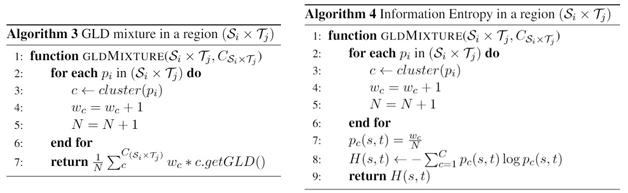
\includegraphics{figs/Algorithms_3_4.png}
\end{figure}

\subsection{Information entropy as a measure of uncertainty in a spatio-temporal region}
\label{sub:InfomationEntropyRegionWorkflow}
Now, what happens if we want to measure the uncertainty quantitatively? The information entropy is useful in this context. We use the different clusters we got in Section \ref{Clusterizing the GLD based in its lambda values} as the different outcomes of the system. The information entropy is computed as follows $H(s,t)=-\sum_{c=1}^C p_{c}(s,t)\log p_{c}(s,t)$, where $c$ represent a particular cluster in the set of clusters $C$, and $p_{c}(s,t)$ represents the probability of occurrence of the cluster $c$ in the spatio-temporal region $(s,t)$.

Algorithm 4 computes the information entropy in a region $C_{(\mathcal{S}_{i} \times \mathcal{T}_{j})}$. In lines 2 to 7, we assess the probability of each cluster in the region. Using this result, we can evaluate the information entropy $H(s, t)$, line 8, and finally, return the result in line 9.


\begin{figure}[!ht]
%\vspace{-1cm}
    \centering
    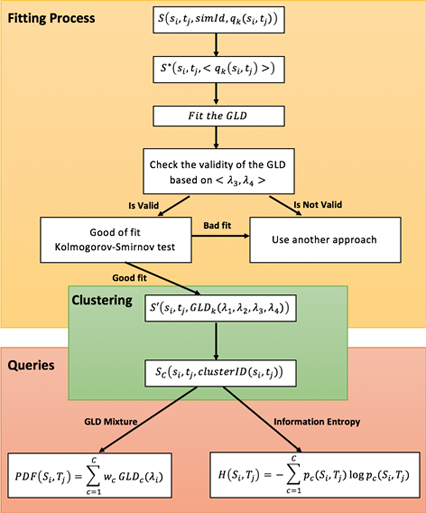
\includegraphics{figs/Diagram.png}
    \caption{SUQ$^2$ workflow divided into three steps, (a) fitting process, (b) clustering of the GLDs and, (c) queries over the results of the clustering process.}
    \label{fig:workflow}
\end{figure}

\section{Experimental Evaluation}
\label{Experiments}
In this section, we first introduce the data used in our experiments. Next, we discuss how we apply the fitting and clustering techniques over the experiment dataset. Then, we present the queries used in the performance evaluation and discuss the results expressed as a mixture of GLDs and values computed using information entropy.

As a case study, we use the HPC4e seismic benchmark, a collection of four 3D models and sixteen associated tests  \footnote{The benchmark can be freely downloaded from https://hpc4e.eu/downloads/} to generate the data of a cube. The models include simple cases that can be used in the development stage of any geophysical imaging practitioner as well as extremely large cases that can only be solved in a reasonable time using supercomputers. The models are generated based on the required size by means of a Matlab/Octave script. The tests can be used to benchmark and compare the capabilities of different and innovative seismic modelling approaches, thus simplifying the task of assessing the algorithmic and computational advantages.



\subsection{Dataset}
In the HPC4e benchmark, the models are designed as sets of 16 layers with constant physical properties. The top layer delineates the topography and the other 15 delineate different layer interface surfaces or horizons. To generate a single cube with dimensions $250\times501\times501$ we can use the values provided in the benchmark. For example, to generate a cube in the $v_{p}(m/s)$ variable we can use the fixed values of Table \ref{tab:valuesOfVp}. The first slice of this cube is shown in Figure \ref{fig:slice1}.

\begin{table}[ht]
\parbox{.45\linewidth}{
\begin{center}
    \begin{tabular}{|l|l|l|l|l|}
    \hline
    \textbf{Layer} & $v_{p}(m/s)$ &   \textbf{Layer} & $v_{p}(m/s)$ \\ \hline
    1     & 1618.92 &  9 & 2712.06\\ \hline
    2     & 1684.08 &  10 & 2532.2\\ \hline
    3     & 1994.35 &  11 & 2841.03\\ \hline
    4     & 2209.71 &   12 & 3169.31\\ \hline
    5     & 2305.55 &   13 & 3169.31\\ \hline
    6     & 2360.95 &  14 & 3642.28\\ \hline
    7     & 2381.95 &   15 & 3659.22\\ \hline
    8     & 2223.41 &   16 & 4000.00\\ \hline
    \end{tabular}
    \caption {Values of $v_{p}$ used in the generation of a single velocity field cube.}
    \label{tab:valuesOfVp}
    \end{center}
%\quad
}
%\end{table}
\parbox{.45\linewidth}{
%\begin{table}[ht]
\begin{center}
\resizebox{0.6\columnwidth}{!}{
    \begin{tabular}{|l|l|l|l|l|l|}
    \hline
    \textbf{Layer} & \textbf{PDF Family} & \textbf{Parameters} & \textbf{Layer} & \textbf{PDF Family}& \textbf{Parameters} \\\hline
    1     & Gaussian & [1619, 711.2] & 9     & Exponential & [3949, 394.9]             \\ \hline 
    2     & Gaussian & [3368, 711.2] & 10   & Exponential & [5983, 711.2]               \\ \hline
    3     & Gaussian & [8839, 711.2] & 11   & Exponential & [3520, 352.0]              \\ \hline
    4     & Gaussian & [7698, 301.5] & 12   & Exponential & [3155, 315.5]              \\ \hline
    5     & Lognormal   & [7723, 294.7] &  13   & Uniform     & [2541, 396.4]              \\ \hline
    6     & Lognormal   & [7733, 292.2] & 14   & Uniform     & [2931, 435.3]              \\ \hline
    7     & Lognormal   & [7658, 312.1] & 15   & Uniform     & [2948, 437.0]             \\ \hline
    8     & Lognormal   & [3687, 368.7] & 16   & Uniform     & [3289, 471.1]              \\ \hline
   \end{tabular}
}
    \caption {PDFs and the parameters used to sample the $v_{p}$ attribute, to generate n velocity models.}
    \label{tab:PDFsOfVp}
    \end{center}
}
\end{table}

As our purpose is to study the uncertainty in the simulation output, we need the input $v_{p}(m/s)$ to present a stochastic behavior. We model the input according to the distributions depicted in Table \ref{tab:PDFsOfVp}. Next, using a Monte Carlo method, we generate a sampling of 1000 realizations of the $v_{p}(m/s)$ variable and use a Matlab script provided by the HPC4e benchmark to generate the cube data. We perform the simulations
1000 times, one for each  realization, and generate 1000 cubes (230 GB) as output. The generated cubes are $250\times501\times501$  multi-dimensional arrays. In order to simplify the computational process and visualize the results, we select the slice 200
to be used in our experiments.
Then, we have 1000 realizations of a slice with size of $250\times501$. The data schema in Equation \ref{eq:data_base_structure} can be simplified as we only have two spatial dimensions and no time domain. Thus, the dataset can be represented as $S(x_{i},y_{j},simId,v_{p}(x_{i},y_{j}))$. In this new representation, $(x_{i},y_{j})$ is the 2D coordinates and $v_{p}(x_{i},y_{j})$ is the velocity value at point $(x_{i},y_{j})$. \textit{simId} represents the Id of the simulation, ranging from 1 to 1000.


\subsection{Fitting the GLD}\label{ft_gld}
The first step is to find the \textit{GLD} that best fits the dataset at each spatial location. Running Algorithm \ref{alg:fitGLD}, we get a new 2D array:
\begin{equation}\label{eq:gld_fit_2D}
S'(x_{i},y_{j},GLD(\lambda_{1}, \lambda_{2}, \lambda_{3}, \lambda_{4}))
\end{equation}
The raw data is significantly reduced and the new dataset is characterized by four lambda values at each spatial location. 

To check how good is the fit, we use the \textit{ks.test} algorithm included in the R-package \textit{stats} \cite{Lopes2011}, which return the \textit{p-value} at each spatial location. Our results show that the fit of the GLD is acceptable in most cases (\textit{p-value} $>0.05$),
%to be more exact, 
in 82 \% of the spatial locations (see Figure \ref{fig:p_values_greater_05}). In the 18\% regions where the GLD modeling was not acceptable, some \textit{GLD} extensions proposed in \cite{Karian2011} could be used. Since the main purpose of this paper is to demonstrate the usefulness of the \textit{GLD} in \textit{UQ}, this particular problem is beyond our scope.

\begin{figure*}[!ht]
\begin{multicols}{2}
    \centering
    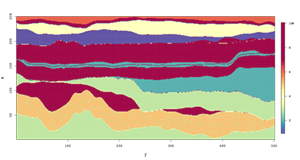
\includegraphics{figs/clusters_slice.png}
    \caption{One slice of the $250\times501\times501$ cube. In the slice, we can distinguish between the different layers.}
    \label{fig:slice1}
    \centering
    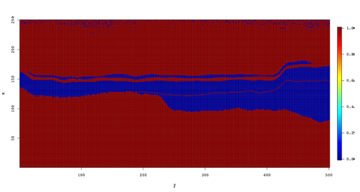
\includegraphics{figs/p_value_greater_05.png}
    \caption{The red color shows where the p-value is greater than 0.05.}
    \label{fig:p_values_greater_05}
\end{multicols}
\end{figure*}

\subsection{Clustering}\label{useCaseClustering}
Up to now, the dataset is characterized by the schema depicted by Equation \ref{eq:gld_fit_2D}. Then, using a clustering algorithm, such as k-means, we group the GLDs based on its $(\lambda_{2}, \lambda_{3}, \lambda_{4})$ values, as discussed in Section \ref{Clusterizing the GLD based in its lambda values}.
In this paper, we use the k-means algorithm with $k=10$. The choice of the clustering algorithm and the parameterization is subject for further investigation and is beyond the scope of this paper.

Once the clustering algorithm is applied, a new dataset is produced. In the new dataset,  for each spatial location, a label indicates the cluster the \textit{GLD} belongs to, as shown (see the schema at Equation \ref{eq:clustersresult}) in Figure \ref{fig:clusters}. Note that in Figure \ref{fig:clusters}, the blue region corresponding to cluster 11 is not a cluster itself. It is rather the region where the \textit{GLD} is not valid (see Section \ref{ft_gld}).

\begin{equation}\label{eq:clustersresult}
S_{\mathcal{C}}(x_{i},y_{j},clusterID, GLD_{x_{i},y_{j}})
\end{equation}

\begin{figure*}[!ht]
%\vspace{-2cm}
\begin{multicols}{2}
    \centering
        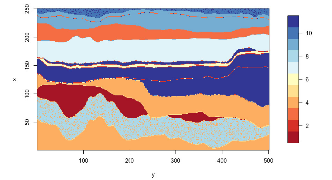
\includegraphics{figs/clusters_image.png}
    \caption{Result of the clustering using k-means with
    $k=10$.}
    \label{fig:clusters}
    \centering
    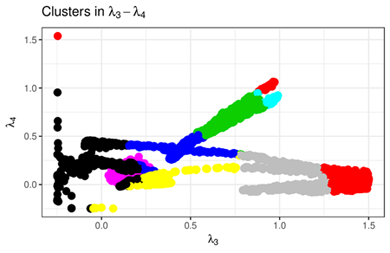
\includegraphics{figs/clusters_l3_l4.png}
    \caption{Distribution of the clusters in the $(\lambda_{3}, \lambda_{4})$ space. The points that belongs to a same cluster are one near the others, as was expected.}
    \label{fig:clusters_lambda3_lambda4_space}
\end{multicols}
\end{figure*}


If we visually compare Figure \ref{fig:slice1} with Figure \ref{fig:clusters}, we observe a close similarity. 

Another interesting result is shown in Figure \ref{fig:clusters_lambda3_lambda4_space}, where we plot the clusters in $(\lambda_{3}, \lambda_{4})$ space. As we mentioned in Section \ref{gldShape}, the shape of the \textit{GLD} depends on the values of $\lambda_{3}$ and $\lambda_{4}$. In this scenario, the expected result is that the members of the same cluster share similar values of $\lambda_{3}$ and $\lambda_{4}$. This is exactly the result we can observe in Figure \ref{fig:clusters_lambda3_lambda4_space}. 

To further corroborate this fact, Figure \ref{fig:cluster1} shows the \textit{PDFs} of 60 members of the 10 clusters. Visually assessing the figures gives an idea of how similar are the shapes of the members of a same cluster and how dissimilar are the shapes of the  members of different clusters. This suggests that our approach is valid. A product of these observations is that we can pick one member of each cluster (the centroid) as a representative of all the members of this cluster, Table \ref{tab:center_of_the_clusters}. The selected member is going to be used to answer the queries in the next Sections.
\begin{table}[ht]
\begin{center}
    \begin{tabular}{|l|l|l|l|l|l|l||l|}
    \hline
    \textbf{Cluster} & $\lambda_{2}$ & $\lambda_{3}$ & $\lambda_{4}$ & \textbf{Cluster} & $\lambda_{2}$ & $\lambda_{3}$ & $\lambda_{4}$  \\ \hline
    1     & 0.0013937313 & 0.9585829 & 1.04696461   &   6 & 0.0003894541 & 1.4076354 & -0.01925743 \\ \hline
    2     & 0.0005291388 & 1.1633978 & -0.07162550  &  7 & 0.0021972784 & 0.3253562 & 0.01493809 \\ \hline
    3     & 0.0020630696 & 0.1349486 & 0.17305941   &  8 & 0.0015421749 & 0.9491101 & 0.86699555 \\ \hline
    4     &  0.0016238358 & 0.8653824 & 0.83857646  &  9  & 0.0018672401 & 0.2176002 & 0.17862024  \\ \hline
    5     & 0.0027346929 & 0.5084664 & 0.39199164  &  10   & 0.4856397733 & 0.1404140 & 0.14011298  \\ \hline
    \end{tabular}
 \caption {Clusters centroids.}
 \label{tab:center_of_the_clusters}
 \end{center}
\end{table}

%\vspace{-5cm}
\begin{figure}[!ht]
%\vspace{-2cm}
    \centering
    %\includegraphics[scale=0.3]{figs/clusters2_s.png}
    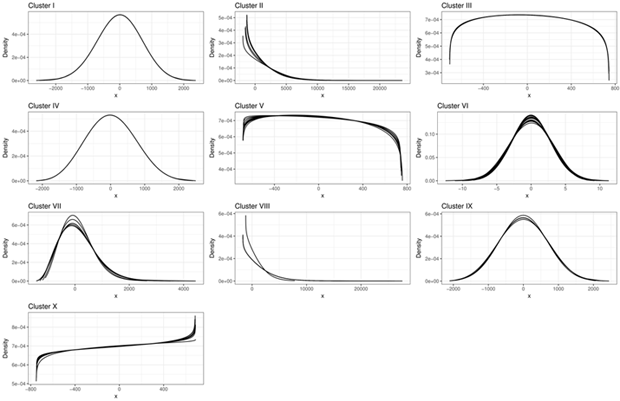
\includegraphics{figs/clusters2.png}
    \caption{\textit{PDFs} of 60 members of the 10 clusters obtained using k-means over the $(\lambda_{2}, \lambda_{3}, \lambda_{4})$ values.}
    \label{fig:cluster1}
%\end{figure}
%\vspace{0.5cm}

%\begin{figure*}
\begin{multicols}{2}
    \centering
    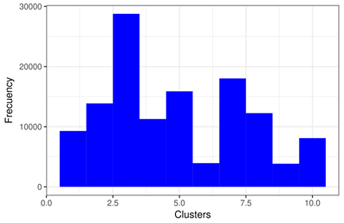
\includegraphics[scale=0.5]{figs/Clusters_histogram.png}
    %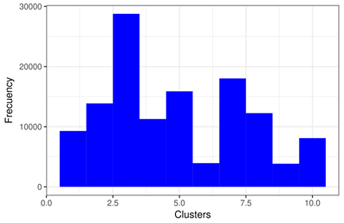
\includegraphics[bb 0 0 794 515]{figs/Clusters_histogram.png}
    \caption{Distribution of the 125250 points by clusters.}
    %\label{fig:clusters}
    \centering
    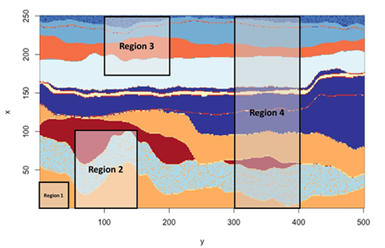
\includegraphics{figs/regions_queries.png}
    \caption{Analysis Regions. The four regions where selected intentionally in this way to warranty different distributions of the clusters inside it.}
\end{multicols}
\end{figure}

The 125250 points of the slice are distributed through the clusters following the histogram of Figure 7.

\subsection{Spatio-temporal queries}
Up to this point, the initial dataset is summarized as depicted by the schema in Equation \ref{eq:clustersresult}. It can be used to answer queries and validate our approach, by comparing the results with the raw data.

First of all, we select four spatio-temporal regions of the dataset where the clusters suggest us different behaviors. The regions are shown in Figure 8. 
With these four regions, we assess the adoption of the \textit{GLD} mixture to obtain the \textit{PDF} that characterizes the uncertainty in a specific  region (see Sections \ref{GLDmixtureresults} and \ref{informationEntropyresults}). We use the information entropy to assign a value that measures the uncertainty at each region. In Section \ref{GLDmixtureresults}, we expect the GLD mixture to characterize well the raw data, and in Section \ref{informationEntropyresults}, we hope that the information entropy is zero in region 1 and increases between regions 2, 3 and 4.

\subsubsection{GLD mixture}\label{GLDmixtureresults}
In this experiment, we use the representative \textit{GLDs} at each cluster and the weight associated to it in the region. Using these parameters, we can build a \textit{GLD mixture} that characterizes the uncertainty on that region. We use
Algorithm 3 described in Section \ref{GLDMixture}. First, we query the region to find  the clusters represented inside it, and how they are distributed. The retrieved results are shown in Table \ref{tab:distribution_of_the_clusters_by_regions}. If we divide the columns of Table \ref{tab:distribution_of_the_clusters_by_regions} by the sum of the elements of each column, we get the weight needed to formulate the \textit{mixed GLDs}. It is clear that the \textit{GLD} in region 1 is represented by the \textit{GLD} of cluster 4. In the other three cases, we get what is shown in the set of 
equations \ref{eq:gld_mix}.


\begin{table}[!ht]
%\vspace{-0.5cm}
\begin{center}
\scalebox{0.6}{
    \begin{tabular}{|l|l|l|l|l|}
    \hline
    \textbf{Cluster} & \textbf{Region 1} &  \textbf{Region 2} &  \textbf{Region 3} &   \textbf{Region 4}  \\ \hline
    1     & 0   		& 2250 & 0 & 979            \\ \hline
    2     & 0   		& 0 & 0 & 268           \\ \hline
    3     & 0      	& 0 & 2596 & 1468       \\ \hline
    4     & 1640	& 4467 & 0 & 5173         \\ \hline
    5     & 0       & 149 & 0 & 269          \\ \hline
    6     & 0     & 0 & 0 & 416           \\ \hline
    7     & 0       & 0 & 1967 & 3920           \\ \hline
    8     & 0     & 3335 & 0 & 3432             \\ \hline
    9     & 0      & 0 & 1918 & 3280       \\ \hline
    10   & 0      & 0 & 901 & 583         \\ \hline
    \end{tabular}}
    \caption {Distribution of the clusters by regions. The four regions are selected intentionally this way to warrant different distributions of the clusters inside it.}
    \label{tab:distribution_of_the_clusters_by_regions}
    \end{center}
\end{table}


\begin{align}
%\vspace{-0.2cm}
\begin{split}
\label{eq:gld_mix}
GLD_{region2} = 0.22GLD_{c1} + 0.44GLD_{c4} + 0.014GLD_{c5} + 0.33GLD_{c8} \\
 GLD_{region3} = 0.34GLD_{c3} + 0.26GLD_{c7} + 0.25GLD_{c9} + 0.12GLD_{c10} \\
 GLD_{region4} = 0.22GLD_{c1} + 0.44GLD_{c4} + 0.014GLD_{c5}  + 0.33GLD_{c8}
\end{split}
\end{align}


Now, we need to evaluate whether the \textit{mixture of GLDs} correctly models the uncertainty in a region. We perform the same \textit{ks-test} used to evaluate the
good quality of the fit, described in Section \ref{gldFitProcess}. Based on the \textit{p-value}, Table \ref{tab:p_values_by_regions}, we can conclude that in all 4 regions the \textit{mixture of GLDs} is a good fit to the raw data.

\begin{table}[ht]
\begin{center}
    \begin{tabular}{|l|l|l|l|l|}
    \hline
    \textbf{Metrics} & \textbf{Region 1} &  \textbf{Region 2} &  \textbf{Region 3} &   \textbf{Region 4}  \\ \hline
    p-value     & 0.73   		& 0.56 & 0.34 & 0.08            \\ \hline
    \end{tabular}
    \caption {p-values by regions.}
    \label{tab:p_values_by_regions}
    \end{center}
\end{table}



\subsubsection{Information Entropy}\label{informationEntropyresults}

Based on the distribution of clusters inside the regions (see Table \ref{tab:distribution_of_the_clusters_by_regions}), we can compute the entropy. 

\begin{table}[ht]
\begin{center}
    \begin{tabular}{|l|l|l|l|l|}
    \hline
    \textbf{entropy} & \textbf{Region 1} &  \textbf{Region 2} &  \textbf{Region 3} &   \textbf{Region 4}  \\ \hline
    value     & 0   		& 1.122243 & 1.41166 & 2.024246            \\ \hline
    \end{tabular}
    \caption {Information Entropy by regions.}
    \label{tab:entropy_by_regions}
    \end{center}
\end{table}

As we expect (see Table \ref{tab:entropy_by_regions}), the entropy in region 1 is zero, because the region contains only members of the cluster 4. On the other regions the entropy increases from region 2 to region 4, as expected. The information entropy is a very good and simple measure of the uncertainty, and here it is demonstrated its usefulness combined with the \textit{GLD}.

 

\section{Conclusion}
\label{Conclusions}

In this paper, we proposed SUQ$^2$, a method to answer uncertainty quantification (UQ) queries over large spatio-temporal simulations. SUQ$^2$ trades large simulation data by probability density functions (PDFs), thus saving huge amount of storage space and computational cost. It enables complex data distribution representation at each simulation point, as much as a  spatio-temporal view  of simulation uncertainty computed by mixing spatial point PDFs.
We evaluated SUQ$^2$ using a seismology use case, considering the computation of uncertainty in regions of a slice of the seismic cube. The results show that SUQ$^2$ method produces an accurate view of the uncertainty in regions of space-time while considerably saving storage space and reducing the cost associated with the PDF modeling of the dataset. To the best of our knowledge, this is the first work to use GLD as the basis for answering UQ queries in spatio-temporal regions and to compile a series of techniques to produce a query answering workflow.



\subsection*{Acknowledgments}
This work has been funded by CNPq, CAPES, FAPERJ, the Inria HPDaSc
and SciDISC Associated Teams and the European Commission (HPC4E H2020) project.


\itemsep=1pt
\begin{thebibliography}{10}
\begin{small}


\bibitem{Tobergte2013}
D. R. Tobergte and S. Curtis.
\newblock {Workshop on Quantification, Communication, and Interpretation of
  Uncertainty in Simulation and Data Science}.
\newblock in {\em Journal of Chemical Information and Modeling}, 53(9):1689--1699,
  2013.


\bibitem{Baroni2014a}
G. Baroni and S. Tarantola.
\newblock {A General Probabilistic Framework for uncertainty and global
  sensitivity analysis of deterministic models: A hydrological case study}.
\newblock in {\em Environmental Modelling and Software}, 51:26--34, 2014.

\bibitem{Johnstone2015}
R. H. Johnstone, E. T. Y. Chang, R. Bardenet, T. P. de~Boer,
  D. J. Gavaghan, P. Pathmanathan, R. H. Clayton, and G. R. Mirams.
\newblock {Uncertainty and variability in models of the cardiac action
  potential: Can we build trustworthy models?}
\newblock in {\em Journal of Molecular and Cellular Cardiology}, 96:49--62, 2016.
  


\bibitem{Karian2011}
Z. A. Karian and E. J. Dudewicz.
\newblock {\em {Handbook of fitting statistical distributions with R}}.
\newblock 2011.


\bibitem{Freimer1988}
M. Freimer, C. T. Lin, and G. S. Mudholkar.
\newblock {A Study Of The Generalized Tukey Lambda Family}.
\newblock in {\em Communications in Statistics - Theory and Methods},
  17(10):3547--3567, 1988.
  
\bibitem{Corlu2016}
C. G. Corlu and M. Meterelliyoz.
\newblock {Estimating the Parameters of the Generalized Lambda Distribution:
  Which Method Performs Best?}
\newblock in {\em Communications in Statistics: Simulation and Computation},
  45(7):2276--2296, 2016.
  

\bibitem{Su2007}
S. Su.
\newblock {Fitting Single and Mixture of Generalized Lambda Distributions to
  Data via Discretized and Maximum Likelihood Methods: GLDEX in R}.
\newblock {\em Journal of Statistical Software}, 21(9), 2007.

\bibitem{Lampasi2006}
D. A. Lampasi, F. Di Nicola, and L. Podesta.
\newblock {Generalized lambda distribution for the expression of measurement
  uncertainty}.
\newblock {\em IEEE Transactions on Instrumentation and Measurement},
  55(4):1281--1287, 2006.
  
\bibitem{Movahedi2013}
M. M. Movahedi, M. R. Lotfi, and M. Nayyeri.
\newblock {A solution to determining the reliability of products Using
  Generalized Lambda Distribution}.
\newblock {\em Research Journal of Recent Sciences Res.J.Recent Sci},
  2(10):41--47, 2013.
  
 \bibitem{Ning2008}
W. Ning, Y. Gao, and E. J. Dudewicz.
\newblock {Fitting mixture distributions using generalized lambda distributions
  and comparison with normal mixtures}.
\newblock {\em American Journal of Mathematical and Management Sciences},
  28(1-2):81--99, 2008.
  
\bibitem{Wellmann2012}
J. F. Wellmann and K. R. Lieb.
\newblock {Uncertainties have a meaning: Information entropy as a quality
  measure for 3-D geological models}.
\newblock {\em Tectonophysics}, 526-529:207--216, 2012.

\bibitem{Liu2019}
J. Liu,N. Lemus, E. Pacitti, F. Porto, P.  Valduriez. \newblock {Parallel computation of PDFs on big spatial data using spark}. \newblock in {em Distributed and Parallel Databases}, pp. 1-28. In press, 10.1007/s10619-019-07260-3, 2019.

\bibitem{Lopes2011}
R. H. C. Lopes  \newblock {Kolmogorov-Smirnov Test.} \newblock in {Lovric M. (eds) International Encyclopedia of Statistical Science. Springer, Berlin, Heidelberg}, 2011.

\bibitem{Ramberg1974} J. S. Ramberg, and B. W. Schmeiser.\newblock {An approximate
method for generating asymmetric random
variables}. \newblock in {em Communications of the ACM}, 17(2), 78–82.
doi:10.1145/360827.360840, 1974.


\end{small}
 \end{thebibliography}
\end{document}

\endinput
%%
%% End of file `elsarticle-template-harv.tex'.

\end{article}

\end{articlesection}

% put the news items below- there can be multiple news sections
% each with its own title
% news will usually have an author as well as a title, 
% e.g. TCDE elections
% news articles are in the same format as letters
% typically, news articles will be stored in a directory called "news"

%\begin{newssection}{News headline}

% insert news items here; news will typically have authors
% see the Sept. 2018 issue for an example

%\begin{news}{news item title}
%{author name}{author affiliation}
%\input{news/news-article.tex}
%\end{news}
%
%\newpage


%\end{newssection}



\begin{callsection}

%  This section will be empty for your version
%
%  Calls for papers section.  Use the callsection environment.
%  Each call for papers is contained in an call environment, where the single 
%  required options to \begin{call} is the name of the conference.
% typically calls are stored in a "calls" directory
%
%\begin{call}{name of conference}
%\centerline{\includegraphics[width=\textwidth, bb= 0 0 590 760]{calls/conference-name.pdf}}
%\end{call}
%\begin{call}{ICDE 2019 Conference}
%\centerline{\includegraphics[width=\textwidth, bb= 0 0 610 790] {../Dec-2018/calls/icde19.pdf}} 
%\centerline{\includegraphics[width=\textwidth, bb= 0 0 590 760] {calls/icde19.pdf}}
%\end{call}
\begin{call}{TCDE Membership Form}
%\centerline{\includegraphics[width=\textwidth, bb= 0 0 610 790]
\centerline{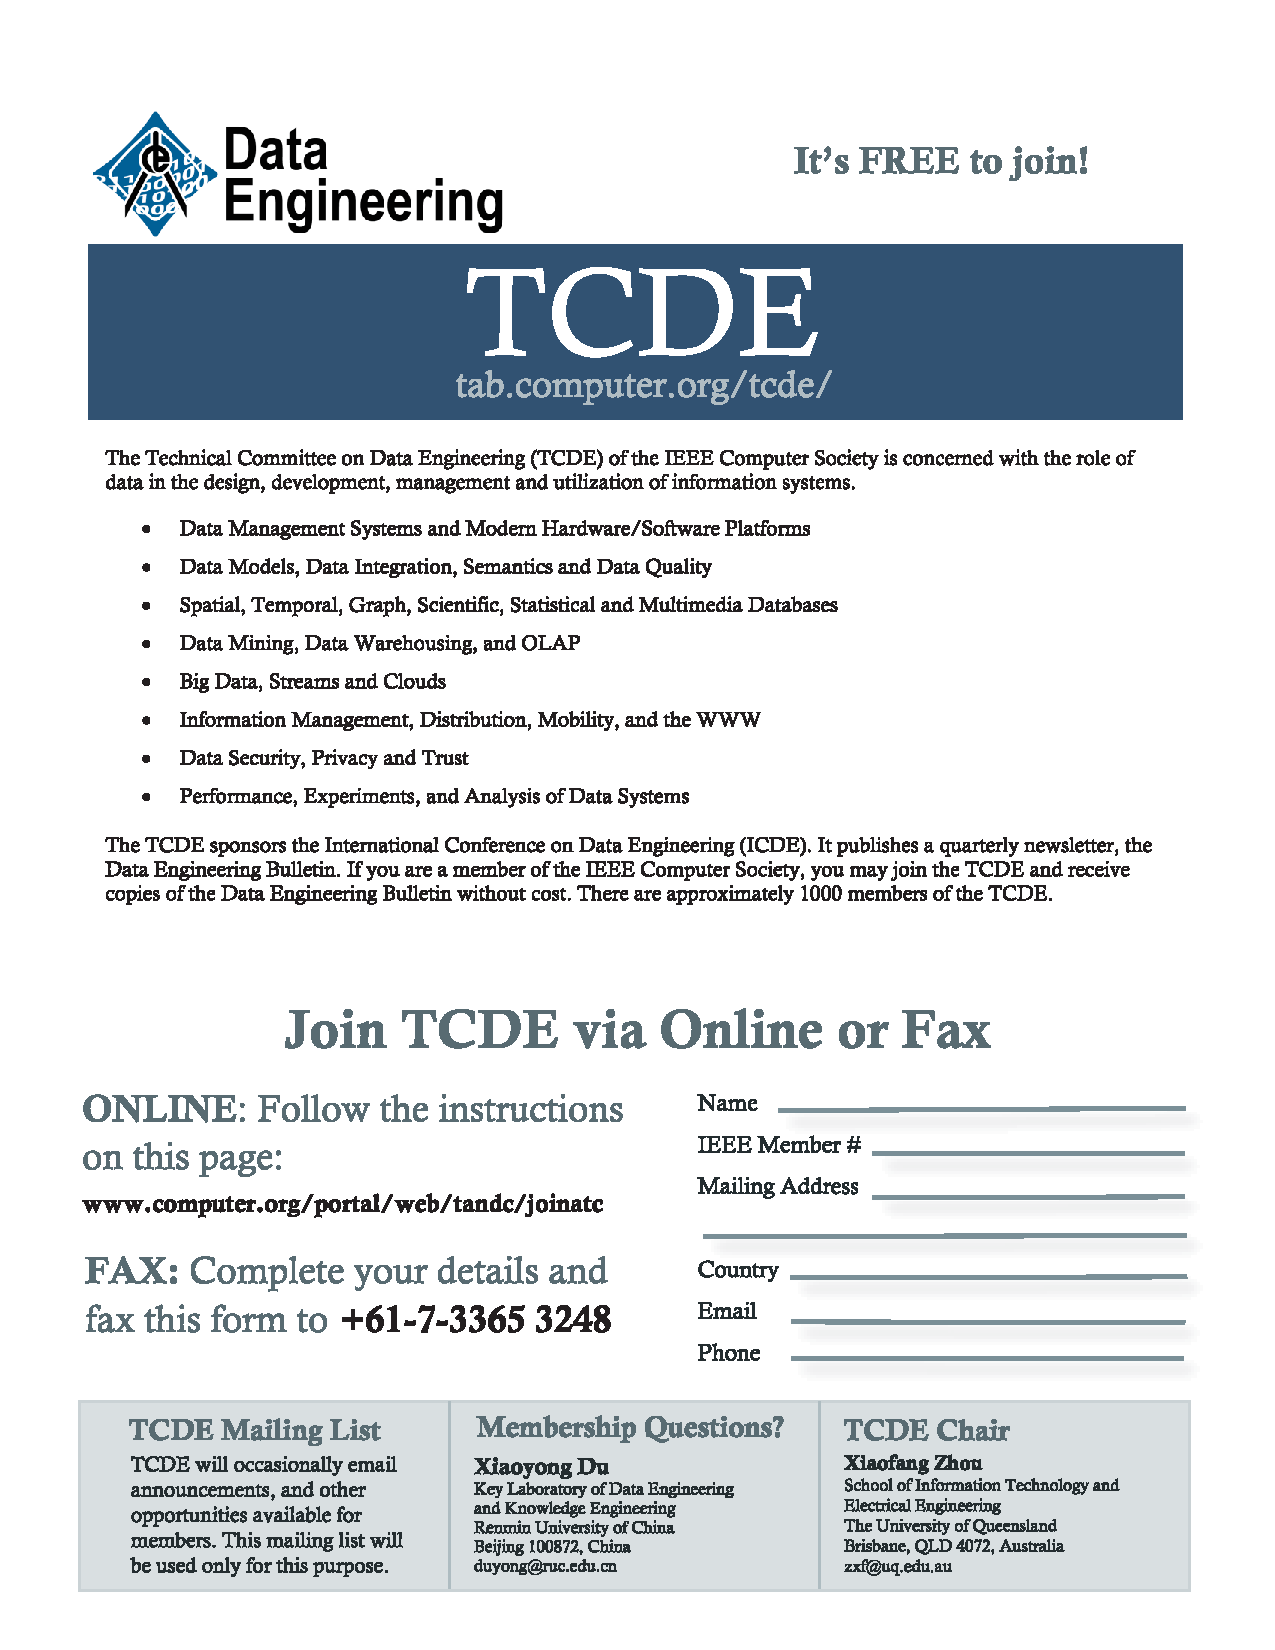
\includegraphics[width=\textwidth, bb= 0 0 590 760] {../Dec-2018/calls/tcde.pdf}}
\end{call}

\end{callsection}

\end{bulletin}
\end{document}
